% generated from JIRA project LVV
% using template at /usr/share/miniconda/envs/docsteady-env/lib/python3.12/site-packages/docsteady/templates/tpr.latex.jinja2.
% using docsteady version 0.0.0
% Please do not edit -- update information in Jira instead
\documentclass[DM,lsstdraft,STR,toc]{lsstdoc}
\usepackage{geometry}
\usepackage{longtable,booktabs}
\usepackage{enumitem}
\usepackage{arydshln}
\usepackage{attachfile}
\usepackage{array}
\usepackage{dashrule}
\usepackage{pdfpages}

\newcolumntype{L}[1]{>{\raggedright\let\newline\\\arraybackslash\hspace{0pt}}p{#1}}

\input{meta.tex}

\newcommand{\attachmentsUrl}{https://github.com/\gitorg/\lsstDocType-\lsstDocNum/blob/\gitref/attachments}
\providecommand{\tightlist}{
  \setlength{\itemsep}{0pt}\setlength{\parskip}{0pt}}

\setcounter{tocdepth}{4}

\providecommand{\ul}[1]{\textbf{#1}}

\begin{document}

\def\milestoneName{Data Management Acceptance Test Campaign, Fall 2023}
\def\milestoneId{}
\def\product{Acceptance}

\setDocCompact{true}

\title{LVV-P106: Data Management Acceptance Test Campaign, Fall 2023 Test Plan and Report}
\setDocRef{\lsstDocType-\lsstDocNum}
\date{ 2024-05-07 }
\author{ Jeffrey Carlin }

% Most recent last
\setDocChangeRecord{
\addtohist{}{2023-07-01}{First draft}{Jeffrey Carlin}
\addtohist{}{2024-04-08}{Test campaign LVV-P106 completed and results approved. DM-40311}{Jeffrey Carlin}
}

\setDocCurator{Jeffrey Carlin}
\setDocUpstreamLocation{\url{https://github.com/lsst-dm/\lsstDocType-\lsstDocNum}}
\setDocUpstreamVersion{\vcsRevision}



\setDocAbstract{
This is the test plan and report for
\textbf{ Data Management Acceptance Test Campaign, Fall 2023},
an LSST milestone pertaining to the Data Management Subsystem.\\
This document is based on content automatically extracted from the Jira test database on \docDate.
The most recent change to the document repository was on \vcsDate.
}


\maketitle

\section{Introduction}
\label{sect:intro}


\subsection{Objectives}
\label{sect:objectives}

 The primary goal of this DM acceptance test campaign will be to verify
priority 1a DMSR (\citeds{LSE-61}) requirements that have not been verified as
part of prior testing and milestones. Any priority 1b, 2, or 3
requirements that have been completed will also be verified.



\subsection{System Overview}
\label{sect:systemoverview}

 This test campaign is intended to verify that the DM system satisfies at
least half of the priority 1a requirements outlined in the Data
Management System Requirements (DMSR;
\href{https://lse-61.lsst.io/}{LSE-61} ), ensuring that we are
progressing toward readiness for the installation and operation of
LSSTCam. Additional DMSR requirements will be verified in later
Acceptance Test Campaigns.\\
\strut \\
\textbf{Applicable Documents:}\\
\citeds{LSE-61}: Data Management System (DMS) Requirements\\
\citeds{LDM-503} Data Management Test Plan\\
\citeds{LDM-639}: Data Management Acceptance Test Specification\\
\strut \\
Tests in this campaign will use data products and artifacts from Data
Preview 0.2, which consists of DESC Data Challenge 2 (DC2) simulated
data reprocessed using the LSST Science Pipelines. Additional on-sky
data from auxTel imaging campaigns, and camera test-stand data, will be
used when appropriate.


\subsection{Document Overview}
\label{sect:docoverview}

This document was generated from Jira, obtaining the relevant information from the
\href{https://jira.lsstcorp.org/secure/Tests.jspa\#/testPlan/LVV-P106}{LVV-P106}
~Jira Test Plan and related Test Cycles (
\href{https://jira.lsstcorp.org/secure/Tests.jspa\#/testCycle/LVV-C260}{LVV-C260}
).

Section \ref{sect:intro} provides an overview of the test campaign, the system under test (\product{}),
the applicable documentation, and explains how this document is organized.
Section \ref{sect:testplan} provides additional information about the test plan, like for example the configuration
used for this test or related documentation.
Section \ref{sect:personnel} describes the necessary roles and lists the individuals assigned to them.

Section \ref{sect:overview} provides a summary of the test results, including an overview in Table \ref{table:summary},
an overall assessment statement and suggestions for possible improvements.
Section \ref{sect:detailedtestresults} provides detailed results for each step in each test case.

The current status of test plan \href{https://jira.lsstcorp.org/secure/Tests.jspa\#/testPlan/LVV-P106}{LVV-P106} in Jira is \textbf{ Completed }.

\subsection{References}
\label{sect:references}
\renewcommand{\refname}{}
\bibliography{lsst,refs,books,refs_ads,local}


\newpage
\section{Test Plan Details}
\label{sect:testplan}


\subsection{Data Collection}

  Observing is not required for this test campaign.

\subsection{Verification Environment}
\label{sect:hwconf}
  Most testing will be performed using the Rubin Science Platform (RSP)
and the development cluster at the USDF. In particular, we will use
version 26 of the Pipelines for most tests; some tests will use more
recent weekly builds of the Pipelines.




\subsection{Related Documentation}


No additional documentation provided.


\subsection{PMCS Activity}

Primavera milestones related to the test campaign:
\begin{itemize}
\item None
\end{itemize}


\newpage
\section{Personnel}
\label{sect:personnel}

The personnel involved in the test campaign is shown in the following table.

{\small
\begin{longtable}{p{3cm}p{3cm}p{3cm}p{6cm}}
\hline
\multicolumn{2}{r}{T. Plan \href{https://jira.lsstcorp.org/secure/Tests.jspa\#/testPlan/LVV-P106}{LVV-P106} owner:} &
\multicolumn{2}{l}{\textbf{ Jeffrey Carlin } }\\\hline
\multicolumn{2}{r}{T. Cycle \href{https://jira.lsstcorp.org/secure/Tests.jspa\#/testCycle/LVV-C260}{LVV-C260} owner:} &
\multicolumn{2}{l}{\textbf{
Jeffrey Carlin }
} \\\hline
\textbf{Test Cases} & \textbf{Assigned to} & \textbf{Executed by} & \textbf{Additional Test Personnel} \\ \hline
\href{https://jira.lsstcorp.org/secure/Tests.jspa#/testCase/LVV-T146}{LVV-T146}
& {\small Leanne Guy } & {\small Leanne Guy } &
\begin{minipage}[]{6cm}
\smallskip
{\small  }
\medskip
\end{minipage}
\\ \hline
\href{https://jira.lsstcorp.org/secure/Tests.jspa#/testCase/LVV-T1240}{LVV-T1240}
& {\small Jim Bosch } & {\small Jeffrey Carlin } &
\begin{minipage}[]{6cm}
\smallskip
{\small  }
\medskip
\end{minipage}
\\ \hline
\href{https://jira.lsstcorp.org/secure/Tests.jspa#/testCase/LVV-T132}{LVV-T132}
& {\small Leanne Guy } & {\small Jeffrey Carlin } &
\begin{minipage}[]{6cm}
\smallskip
{\small  }
\medskip
\end{minipage}
\\ \hline
\href{https://jira.lsstcorp.org/secure/Tests.jspa#/testCase/LVV-T62}{LVV-T62}
& {\small Jim Bosch } & {\small Jeffrey Carlin } &
\begin{minipage}[]{6cm}
\smallskip
{\small  }
\medskip
\end{minipage}
\\ \hline
\href{https://jira.lsstcorp.org/secure/Tests.jspa#/testCase/LVV-T41}{LVV-T41}
& {\small Jim Bosch } & {\small Jeffrey Carlin } &
\begin{minipage}[]{6cm}
\smallskip
{\small  }
\medskip
\end{minipage}
\\ \hline
\href{https://jira.lsstcorp.org/secure/Tests.jspa#/testCase/LVV-T97}{LVV-T97}
& {\small Kian-Tat Lim } & {\small Jeffrey Carlin } &
\begin{minipage}[]{6cm}
\smallskip
{\small  }
\medskip
\end{minipage}
\\ \hline
\href{https://jira.lsstcorp.org/secure/Tests.jspa#/testCase/LVV-T1946}{LVV-T1946}
& {\small Jeffrey Carlin } & {\small Jeffrey Carlin } &
\begin{minipage}[]{6cm}
\smallskip
{\small  }
\medskip
\end{minipage}
\\ \hline
\href{https://jira.lsstcorp.org/secure/Tests.jspa#/testCase/LVV-T1947}{LVV-T1947}
& {\small Jeffrey Carlin } & {\small Jeffrey Carlin } &
\begin{minipage}[]{6cm}
\smallskip
{\small  }
\medskip
\end{minipage}
\\ \hline
\href{https://jira.lsstcorp.org/secure/Tests.jspa#/testCase/LVV-T28}{LVV-T28}
& {\small Colin Slater } & {\small Jeffrey Carlin } &
\begin{minipage}[]{6cm}
\smallskip
{\small  }
\medskip
\end{minipage}
\\ \hline
\href{https://jira.lsstcorp.org/secure/Tests.jspa#/testCase/LVV-T142}{LVV-T142}
& {\small Colin Slater } & {\small Jeffrey Carlin } &
\begin{minipage}[]{6cm}
\smallskip
{\small  }
\medskip
\end{minipage}
\\ \hline
\href{https://jira.lsstcorp.org/secure/Tests.jspa#/testCase/LVV-T1748}{LVV-T1748}
& {\small Jeffrey Carlin } & {\small Jeffrey Carlin } &
\begin{minipage}[]{6cm}
\smallskip
{\small  }
\medskip
\end{minipage}
\\ \hline
\href{https://jira.lsstcorp.org/secure/Tests.jspa#/testCase/LVV-T1759}{LVV-T1759}
& {\small Jeffrey Carlin } & {\small Jeffrey Carlin } &
\begin{minipage}[]{6cm}
\smallskip
{\small  }
\medskip
\end{minipage}
\\ \hline
\href{https://jira.lsstcorp.org/secure/Tests.jspa#/testCase/LVV-T1758}{LVV-T1758}
& {\small Jeffrey Carlin } & {\small Jeffrey Carlin } &
\begin{minipage}[]{6cm}
\smallskip
{\small  }
\medskip
\end{minipage}
\\ \hline
\href{https://jira.lsstcorp.org/secure/Tests.jspa#/testCase/LVV-T149}{LVV-T149}
& {\small Leanne Guy } & {\small Jeffrey Carlin } &
\begin{minipage}[]{6cm}
\smallskip
{\small  }
\medskip
\end{minipage}
\\ \hline
\href{https://jira.lsstcorp.org/secure/Tests.jspa#/testCase/LVV-T40}{LVV-T40}
& {\small Jeffrey Carlin } & {\small Jeffrey Carlin } &
\begin{minipage}[]{6cm}
\smallskip
{\small  }
\medskip
\end{minipage}
\\ \hline
\end{longtable}
}

\newpage

\section{Test Campaign Overview}
\label{sect:overview}

\subsection{Summary}
\label{sect:summarytable}

{\small
\begin{longtable}{p{2cm}cp{2.3cm}p{8.6cm}p{2.3cm}}
\toprule
\multicolumn{2}{r}{ T. Plan \href{https://jira.lsstcorp.org/secure/Tests.jspa\#/testPlan/LVV-P106}{LVV-P106}:} &
\multicolumn{2}{p{10.9cm}}{\textbf{ Data Management Acceptance Test Campaign, Fall 2023 }} & Completed \\\hline
\multicolumn{2}{r}{ T. Cycle \href{https://jira.lsstcorp.org/secure/Tests.jspa\#/testCycle/LVV-C260}{LVV-C260}:} &
\multicolumn{2}{p{10.9cm}}{\textbf{ Data Management Acceptance Test Campaign, Fall 2023 }} & Done \\\hline
\textbf{Test Cases} &  \textbf{Ver.} & \textbf{Status} & \textbf{Comment} & \textbf{Issues} \\\toprule
\href{https://jira.lsstcorp.org/secure/Tests.jspa#/testCase/LVV-T146}{LVV-T146}
&  1
\\
 \hfill Execution & LVV-E3318
& Pass &
\begin{minipage}[]{9cm}
\smallskip

\medskip
\end{minipage}
&   \\\hline
\href{https://jira.lsstcorp.org/secure/Tests.jspa#/testCase/LVV-T1240}{LVV-T1240}
&  1
\\
 \hfill Execution & LVV-E3193
& Pass &
\begin{minipage}[]{9cm}
\smallskip
Test executed with science pipelines version w\_2023\_37 in the RSP
Notebook aspect at the USDF.\\
\strut \\
The executed notebook was saved in the repository associated with this
campaign's test report as ``notebooks/test\_LVV-T40\_T1240.ipynb''.
\medskip
\end{minipage}
&   \\\hline
\href{https://jira.lsstcorp.org/secure/Tests.jspa#/testCase/LVV-T132}{LVV-T132}
&  1
\\
 \hfill Execution & LVV-E3057
& Pass &
\begin{minipage}[]{9cm}
\smallskip

\medskip
\end{minipage}
&   \\\hline
\href{https://jira.lsstcorp.org/secure/Tests.jspa#/testCase/LVV-T62}{LVV-T62}
&  2
\\
 \hfill Execution & LVV-E3058
& Pass &
\begin{minipage}[]{9cm}
\smallskip
Test executed with science pipelines version w\_2023\_34 in the RSP
Notebook aspect at the USDF.\\
\strut \\
The executed notebook was saved in the repository associated with this
campaign's test report as ``notebooks/test\_LVV-T62.ipynb''.
\medskip
\end{minipage}
&   \\\hline
\href{https://jira.lsstcorp.org/secure/Tests.jspa#/testCase/LVV-T41}{LVV-T41}
&  1
\\
 \hfill Execution & LVV-E3056
& Pass &
\begin{minipage}[]{9cm}
\smallskip
Test executed with science pipelines version w\_2023\_37 in the RSP
Notebook aspect at the USDF.\\
\strut \\
The executed notebook was saved in the repository associated with this
campaign's test report as ``notebooks/test\_LVV-T41.ipynb''.
\medskip
\end{minipage}
&   \\\hline
\href{https://jira.lsstcorp.org/secure/Tests.jspa#/testCase/LVV-T97}{LVV-T97}
&  1
\\
 \hfill Execution & LVV-E3002
& Pass &
\begin{minipage}[]{9cm}
\smallskip
Executed at the USDF using the w\_2023\_43 version of the Science
Pipelines.\\
\strut \\
In addition to demonstrating that changing the "RELEASE\_ID" results in
unique IDs, we further examine the code itself to demonstrate that the
uniqueness of IDs is ensured by the way the code is implemented.\\
\strut \\
The implementation of how the 64 bits of the Source/Object IDs are
apportioned is in the
\texttt{\_IdGeneratorBits}\href{https://github.com/lsst/meas_base/blob/1bfaca56951770c88f4308da41de16d72ce40db9/python/lsst/meas/base/_id_generator.py\#L507-L537}{~class},
and especially its \texttt{\_\_post\_init\_\_}:\\

\begin{itemize}
\tightlist
\item
  it gets the maximum number of bits needed to pack the data ID (based
  on \texttt{\{visit,\ detector\}} for Source, and
  \texttt{\{tract,\ patch\}} for Object) and turns that into the number
  of distinct data IDs it could hold \texttt{(n\_data\_ids)};
\item
  it multiplies that with the \texttt{n\_releases} option to identify
  how many "upper" bits need to be reserved for
  \texttt{n\_data\_ids*n\_releases} "catalog\_ids", and sets
  \texttt{n\_counters} to be the number of values remaining in the
  Source or Object 64-bit ID to count sources or objects within one
  image.
\end{itemize}

\hfill\break
Because some interfaces historically wanted to count bits rather than
just multiply integers, there is a mix of direct multiplication and log2
addition. But you can see the result most clearly in
\texttt{FullIdGenerator.arange} and
\texttt{FullIdGenerator.catalog\_id}; a full Source or Object ID is:\\

\begin{verbatim}
id = counter + n_counters * catalog_id
\end{verbatim}

or\\

\begin{verbatim}
id = counter + n_counters * (packed_data_id + n_data_ids * release_id)
\end{verbatim}

\hfill\break
and hence the releases will get distinct IDs as long as counter values
are less than \texttt{n\_counters} and the packed data IDs are less than
\texttt{n\_data\_ids}. (And there are several checks throughout the file
for those criteria).
\medskip
\end{minipage}
&   \\\hline
\href{https://jira.lsstcorp.org/secure/Tests.jspa#/testCase/LVV-T1946}{LVV-T1946}
&  1
\\
 \hfill Execution & LVV-E2982
& Pass &
\begin{minipage}[]{9cm}
\smallskip
This test case can be executed by running the script test\_LVV-T1946.py,
which is available in the test report github
repository\textquotesingle s "scripts/" directory.\\
\strut \\
The tests that confirm fluxes have "reasonable" values are checking that
the fluxes, if converted to magnitudes, would result in a magnitude
fainter than -5.
\medskip
\end{minipage}
&   \\\hline
\href{https://jira.lsstcorp.org/secure/Tests.jspa#/testCase/LVV-T1947}{LVV-T1947}
&  1
\\
 \hfill Execution & LVV-E2983
& Pass &
\begin{minipage}[]{9cm}
\smallskip
This test case can be executed by running the scripts
test\_LVV-T1947\_DiaSource.py,
~test\_LVV-T1947\_forcedSourceOnDiaObject.py, and
test\_LVV-T1947\_DiaObject.py, which are available in the test report
github repository\textquotesingle s "scripts/" directory.\\
\strut \\
The tests that confirm fluxes have "reasonable" values are checking that
the fluxes, if converted to magnitudes, would result in a magnitude
fainter than -5.
\medskip
\end{minipage}
&   \\\hline
\href{https://jira.lsstcorp.org/secure/Tests.jspa#/testCase/LVV-T28}{LVV-T28}
&  1
\\
 \hfill Execution & LVV-E2984
& Pass &
\begin{minipage}[]{9cm}
\smallskip
This test case can be executed by running the scripts test\_LVV-T28.py,
test\_LVV-T28\_forcedSource.py, and test\_LVV-T28\_DC2.py, which are
available in the test report github repository\textquotesingle s
"scripts/" directory.\\
\strut \\
The tests that confirm fluxes have "reasonable" values are checking that
the fluxes, if converted to magnitudes, would result in a magnitude
fainter than -5.
\medskip
\end{minipage}
&   \\\hline
\href{https://jira.lsstcorp.org/secure/Tests.jspa#/testCase/LVV-T142}{LVV-T142}
&  1
\\
 \hfill Execution & LVV-E2974
& Pass &
\begin{minipage}[]{9cm}
\smallskip
Executed at the USDF using the w\_2023\_43 version of the Science
Pipelines.
\medskip
\end{minipage}
&   \\\hline
\href{https://jira.lsstcorp.org/secure/Tests.jspa#/testCase/LVV-T1748}{LVV-T1748}
&  1
\\
 \hfill Execution & LVV-E2973
& Pass &
\begin{minipage}[]{9cm}
\smallskip

\medskip
\end{minipage}
&   \\\hline
\href{https://jira.lsstcorp.org/secure/Tests.jspa#/testCase/LVV-T1759}{LVV-T1759}
&  1
\\
 \hfill Execution & LVV-E2970
& Pass &
\begin{minipage}[]{9cm}
\smallskip
This test used a modified version of the analysis\_tools pipeline
"matchedVisitQualityCore.yaml."
\medskip
\end{minipage}
&   \\\hline
\href{https://jira.lsstcorp.org/secure/Tests.jspa#/testCase/LVV-T1758}{LVV-T1758}
&  1
\\
 \hfill Execution & LVV-E2971
& Pass &
\begin{minipage}[]{9cm}
\smallskip
Note that because we do not have access to u-band data, this test was
performed for only y- and z-band. The steps would be unchanged for
u-band data.
\medskip
\end{minipage}
&   \\\hline
\href{https://jira.lsstcorp.org/secure/Tests.jspa#/testCase/LVV-T149}{LVV-T149}
&  1
\\
 \hfill Execution & LVV-E2972
& Pass &
\begin{minipage}[]{9cm}
\smallskip
Executed using the IDF Notebook, Portal, and API aspects. For the
notebook execution, we used science pipelines version w\_2023\_34.
\medskip
\end{minipage}
&   \\\hline
\href{https://jira.lsstcorp.org/secure/Tests.jspa#/testCase/LVV-T40}{LVV-T40}
&  1
\\
 \hfill Execution & LVV-E2962
& Pass &
\begin{minipage}[]{9cm}
\smallskip
Test executed with science pipelines version w\_2023\_37 in the RSP
Notebook aspect at the USDF.\\
\strut \\
The executed notebook was saved in the repository associated with this
campaign's test report as ``notebooks/test\_LVV-T40\_T1240.ipynb''.
\medskip
\end{minipage}
&   \\\hline
\caption{Test Campaign Summary}
\label{table:summary}
\end{longtable}
}

\subsection{Overall Assessment}
\label{sect:overallassessment}

In this test campaign, we have successfully verified 9 unique
requirements from \citeds{LSE-61} via the execution of 15 Test Cases (all of
which passed). Of these requirements, 6 are of priority 1a, and 3 are
priority 1b. The set of requirements tested in this campaign mostly
cover aspects of the DM system related to the software pipelines and the
facilities for data processing and handling. These tests were performed
at the US Data Facility (USDF) using precursor HSC and Auxtel data.

\subsection{Recommended Improvements}
\label{sect:recommendations}

Not yet available.

\newpage
\section{Detailed Test Results}
\label{sect:detailedtestresults}

\subsection{Test Cycle LVV-C260 }

Open test cycle {\it \href{https://jira.lsstcorp.org/secure/Tests.jspa#/testrun/LVV-C260}{Data Management Acceptance Test Campaign, Fall 2023}} in Jira.

Test Cycle name: Data Management Acceptance Test Campaign, Fall 2023\\
Status: Done

This test cycle verifies a subset of
\href{https://lse-61.lsst.io/}{DMSR} (\citeds{LSE-61}) requirements in order to
verify their completion and readiness for LSST Operations (i.e., that
the requirements laid out in \citeds{LSE-61} have been met by the DM Systems).
Testing will use data products and artifacts from Data Preview 0.2
reprocessing of DESC DC2 data, Auxtel data, and other data products
housed at the U.S. Data Facility (USDF).

\subsubsection{Software Version/Baseline}
Primarily using Science Pipelines version 26 at the USDF.~

\subsubsection{Configuration}
Not provided.

\subsubsection{Test Cases in LVV-C260 Test Cycle}

\paragraph{ LVV-T146 - Verify implementation of DMS Initialization Component }\mbox{}\\

Version \textbf{1}.
Status \textbf{Approved}.
Open  \href{https://jira.lsstcorp.org/secure/Tests.jspa#/testCase/LVV-T146}{\textit{ LVV-T146 } }
test case in Jira.

Demonstrate that all components of the DM system have a defined
deployment configuration within the DM deployment strategy

\textbf{ Preconditions}:\\


Execution status: {\bf  }

Final comment:\\



Detailed steps results LVV-C260-LVV-T146 LVV-E3318-3713:\\
{\bf Note:} Steps "Not Executed" and with No Result are not shown in this report.\\
\begin{tabular}{p{4cm}p{12cm}}
\toprule
Step LVV-E3318-1 & Step Execution Status: \textbf{ Pass } \\ \hline
\end{tabular}
 Description \\
{\footnotesize
Inspect each service component to check if it has a deployment
configuration defined

}
\hdashrule[0.5ex]{\textwidth}{1pt}{3mm}
  Expected Result \\
{\footnotesize
All systems have a defined deployment configuration as part of the DM
deployment strategy\\
\strut \\

}
\hdashrule[0.5ex]{\textwidth}{1pt}{3mm}
  Actual Result \\
{\footnotesize
\begin{longtable}[]{@{}
  >{\raggedright\arraybackslash}p{(\columnwidth - 6\tabcolsep) * \real{0.2500}}
  >{\raggedright\arraybackslash}p{(\columnwidth - 6\tabcolsep) * \real{0.2500}}
  >{\raggedright\arraybackslash}p{(\columnwidth - 6\tabcolsep) * \real{0.2500}}
  >{\raggedright\arraybackslash}p{(\columnwidth - 6\tabcolsep) * \real{0.2500}}@{}}
\toprule\noalign{}
\begin{minipage}[b]{\linewidth}\raggedright
Service
\end{minipage} & \begin{minipage}[b]{\linewidth}\raggedright
Location
\end{minipage} & \begin{minipage}[b]{\linewidth}\raggedright
Deployment Strategy
\end{minipage} & \begin{minipage}[b]{\linewidth}\raggedright
Status
\end{minipage} \\
\midrule\noalign{}
\endhead
\bottomrule\noalign{}
\endlastfoot
Archiving~ & Summit, USDF & \begin{minipage}[t]{\linewidth}\raggedright
S3 on Kubernetes. Summit currently ssh/NFS to bare metal machine, which
also comes up in a known/safe state.\\
\strut
\end{minipage} & Deployed \\
Planned Observation Publication (a.k.a. ObsLocTAP) & USDF &
Safir/Phalanx on Kubernetes &
\begin{minipage}[t]{\linewidth}\raggedright
Not Deployed\\
\strut
\end{minipage} \\
Prompt Processing Ingest & USDF &
\begin{minipage}[t]{\linewidth}\raggedright
Kubernetes\\
\strut
\end{minipage} & \begin{minipage}[t]{\linewidth}\raggedright
Deployed\\
\strut
\end{minipage} \\
\begin{minipage}[t]{\linewidth}\raggedright
Observatory Operations Data\\
\strut
\end{minipage} & Summit & \begin{minipage}[t]{\linewidth}\raggedright
Kubernetes\\
\strut
\end{minipage} & \begin{minipage}[t]{\linewidth}\raggedright
Deployed\\
\strut
\end{minipage} \\
\begin{minipage}[t]{\linewidth}\raggedright
Observatory Control System (OCS) Controlled Pipeline\\
\strut
\end{minipage} & Summit & \begin{minipage}[t]{\linewidth}\raggedright
Kubernetes\\
\strut
\end{minipage} & \begin{minipage}[t]{\linewidth}\raggedright
Deployed\\
\strut
\end{minipage} \\
Telemetry Gateway & Summit & Sasquatch/Phalanx/Kafka on Kubernetes &
\begin{minipage}[t]{\linewidth}\raggedright
Deployed\\
\strut
\end{minipage} \\
Prompt Processing & USDF & KNative on Kubernetes &
\begin{minipage}[t]{\linewidth}\raggedright
Deployed\\
\strut
\end{minipage} \\
Alert Distribution & USDF & \begin{minipage}[t]{\linewidth}\raggedright
Kubernetes\\
\strut
\end{minipage} & \begin{minipage}[t]{\linewidth}\raggedright
Tests deployed, operational system not quite\\
\strut
\end{minipage} \\
Prompt Quality Control & USDF &
\begin{minipage}[t]{\linewidth}\raggedright
Part of Prompt Processing payload, with publication to
Sasquatch/Phalanx/Kafka and InfluxDB on K8s\\
\strut
\end{minipage} & \begin{minipage}[t]{\linewidth}\raggedright
Deployed\\
\strut
\end{minipage} \\
Batch Production & USDF & \begin{minipage}[t]{\linewidth}\raggedright
The batch system is independent. It uses Slurm not on K8s and has its
own power-up safe state. ~PanDA and its RCEs are either on K8s or are
like Slurm.\\
\strut
\end{minipage} & \begin{minipage}[t]{\linewidth}\raggedright
Deployed\\
\strut
\end{minipage} \\
Offline QC & USDF & \begin{minipage}[t]{\linewidth}\raggedright
Part of Batch Production payloads, with publication to
Sasquatch/Phalanx/Kafka and InfluxDB on K8s\\
\strut
\end{minipage} & \begin{minipage}[t]{\linewidth}\raggedright
Deployed\\
\strut
\end{minipage} \\
Bulk Distribution & USDF & \begin{minipage}[t]{\linewidth}\raggedright
Rucio/FTS3 on K8s\\
\strut
\end{minipage} & \begin{minipage}[t]{\linewidth}\raggedright
Deployed\\
\strut
\end{minipage} \\
Data Backbone & USDF & \begin{minipage}[t]{\linewidth}\raggedright
Rucio/FTS3 + ingested on K8s\\
\strut
\end{minipage} & \begin{minipage}[t]{\linewidth}\raggedright
Deployed\\
\strut
\end{minipage} \\
\begin{minipage}[t]{\linewidth}\raggedright
RSP Portal\\
\strut
\end{minipage} & \begin{minipage}[t]{\linewidth}\raggedright
Summit, USDF\\
\strut
\end{minipage} & \begin{minipage}[t]{\linewidth}\raggedright
Phalanx on K8s\\
\strut
\end{minipage} & \begin{minipage}[t]{\linewidth}\raggedright
Deployed\\
\strut
\end{minipage} \\
\begin{minipage}[t]{\linewidth}\raggedright
RSP Notebook\\
\strut
\end{minipage} & \begin{minipage}[t]{\linewidth}\raggedright
Summit, USDF\\
\strut
\end{minipage} & \begin{minipage}[t]{\linewidth}\raggedright
Phalanx on K8s\\
\strut
\end{minipage} & \begin{minipage}[t]{\linewidth}\raggedright
Deployed\\
\strut
\end{minipage} \\
\begin{minipage}[t]{\linewidth}\raggedright
RSP Web API\\
\strut
\end{minipage} & \begin{minipage}[t]{\linewidth}\raggedright
Summit, USDF\\
\strut
\end{minipage} & \begin{minipage}[t]{\linewidth}\raggedright
Phalanx on K8s\\
\strut
\end{minipage} & \begin{minipage}[t]{\linewidth}\raggedright
Deployed\\
\strut
\end{minipage} \\
\end{longtable}

}

\paragraph{ LVV-T1240 - Verify implementation of minimum astrometric standards per CCD }\mbox{}\\

Version \textbf{1}.
Status \textbf{Approved}.
Open  \href{https://jira.lsstcorp.org/secure/Tests.jspa#/testCase/LVV-T1240}{\textit{ LVV-T1240 } }
test case in Jira.

Verify that each CCD in a processed dataset had its astrometric solution
determined by at least~\textbf{astrometricMinStandards = 5~}astrometric
standards.

\textbf{ Preconditions}:\\


Execution status: {\bf  }

Final comment:\\



Detailed steps results LVV-C260-LVV-T1240 LVV-E3193-3588:\\
{\bf Note:} Steps "Not Executed" and with No Result are not shown in this report.\\
\begin{tabular}{p{4cm}p{12cm}}
\toprule
Step LVV-E3193-1 & Step Execution Status: \textbf{ Pass } \\ \hline
\end{tabular}
 Description \\
{\footnotesize
Identify an appropriate processed dataset for this test.

}
\hdashrule[0.5ex]{\textwidth}{1pt}{3mm}
  Expected Result \\
{\footnotesize
A dataset with Processed Visit Images.

}
\hdashrule[0.5ex]{\textwidth}{1pt}{3mm}
  Actual Result \\
{\footnotesize
For this test we use the most recent reprocessing of the Subaru+HSC RC2
dataset. The data were processed with the w\_2023\_32 pipelines.

}
\begin{tabular}{p{4cm}p{12cm}}
\toprule
Step LVV-E3193-2 & Step Execution Status: \textbf{ Pass } \\ \hline
\end{tabular}
 Description \\
{\footnotesize
Identify the path to the data repository, which we will refer to as
\textquotesingle DATA/path\textquotesingle, then execute the following:

}
\hdashrule[0.5ex]{\textwidth}{1pt}{3mm}
  Example Code \\
{\footnotesize
\begin{verbatim}
from lsst.daf.butler import Butler
repo = 'Data/path'
collection = 'collection'
butler = Butler(repo, collections=collection)
\end{verbatim}

}
\hdashrule[0.5ex]{\textwidth}{1pt}{3mm}
  Expected Result \\
{\footnotesize
Butler repo available for reading.

}
\hdashrule[0.5ex]{\textwidth}{1pt}{3mm}
  Actual Result \\
{\footnotesize
Butler access is as follows:\\
repo = \textquotesingle/repo/main\textquotesingle{}\\
rc2\_collection =
\textquotesingle HSC/runs/RC2/w\_2023\_32/DM-40356\textquotesingle{}\\
butler = Butler(repo, collections=rc2\_collection)

}
\begin{tabular}{p{4cm}p{12cm}}
\toprule
Step LVV-E3193-3 & Step Execution Status: \textbf{ Pass } \\ \hline
\end{tabular}
 Description \\
{\footnotesize
Select a single visit from the dataset, and extract its calibration
data. For a subset of CCDs, check how many astrometric standards
contributed to the solution. Confirm that this number is at
least~\textbf{astrometricMinStandards = 5.}

}
\hdashrule[0.5ex]{\textwidth}{1pt}{3mm}
  Expected Result \\
{\footnotesize
At least \textbf{astrometricMinStandards} from each CCD\textbf{~}were
used in determining the WCS solution.

}
\hdashrule[0.5ex]{\textwidth}{1pt}{3mm}
  Actual Result \\
{\footnotesize
This was done 500 times, extracting the source list and WCS for 500
randomly-selected CCD/visit combinations from the repository.\\
\strut \\
It was confirmed that all CCDs selected had more than
astrometricMinStandards=5 standards used in their WCS solutions. This
was done using the following code to extract the number of astrometric
standards for each image:\\
\strut \\
astrom\_selection = np.where(src{[}'calib\_astrometry\_used'{]} ==
True)\\
num\_calib\_astrom.append(np.size(astrom\_selection))\\
\strut \\
In the end, we calculate the fraction of fields that met this
requirement, using:\\
wcsFlagsPercent = (np.size(np.where(num\_calib\_astrom \textgreater{}
5))/np.size(num\_calib\_astrom))*100.0*u.percent\\
\strut \\
The result (from the notebook) is:\\
Percentage of fields with \textgreater{} astrometricMinStandards=5:
100.0 \% -\/- True

}

\paragraph{ LVV-T132 - Verify implementation of Pre-cursor and Real Data }\mbox{}\\

Version \textbf{1}.
Status \textbf{Approved}.
Open  \href{https://jira.lsstcorp.org/secure/Tests.jspa#/testCase/LVV-T132}{\textit{ LVV-T132 } }
test case in Jira.

Demonstrate that pixel-oriented data from astronomical imaging cameras
(precursor or otherwise) can be processed using LSST Science Algorithms
and organized for access through the Data Butler Access Client. ~

\textbf{ Preconditions}:\\


Execution status: {\bf  }

Final comment:\\



Detailed steps results LVV-C260-LVV-T132 LVV-E3057-3452:\\
{\bf Note:} Steps "Not Executed" and with No Result are not shown in this report.\\
\begin{tabular}{p{4cm}p{12cm}}
\toprule
Step LVV-E3057-1 & Step Execution Status: \textbf{ Pass } \\ \hline
\end{tabular}
 Description \\
{\footnotesize
Confirm that the CI jobs used to test DRP processing successfully run.
These jobs use precursor datasets from cameras other than LSST.

}
\hdashrule[0.5ex]{\textwidth}{1pt}{3mm}
  Expected Result \\
{\footnotesize

}
\hdashrule[0.5ex]{\textwidth}{1pt}{3mm}
  Actual Result \\
{\footnotesize
Because the outputs from CI jobs are not persisted, we instead use the
regularly-reprocessed HSC RC2 data. Specifically, we used the output
repo from HSC-RC2 data processing, as executed using a recent weekly
pipelines release (w\_2023\_39). The output repo is tagged with the Jira
ticket number DM-40985.\\
\strut \\
The butler collection within /repo/main at the USDF is
``HSC/runs/RC2/w\_2023\_39/DM-40985\textquotesingle\textquotesingle.

}
\begin{tabular}{p{4cm}p{12cm}}
\toprule
Step LVV-E3057-2 & Step Execution Status: \textbf{ Pass } \\ \hline
\end{tabular}
 Description \\
{\footnotesize
For the precursor dataset, instantiate the Butler, load the data
products, and confirm that they exist as expected.

}
\hdashrule[0.5ex]{\textwidth}{1pt}{3mm}
  Expected Result \\
{\footnotesize
Processed images, catalogs, calibration information, and other related
data products are present and accessible via the Butler.

}
\hdashrule[0.5ex]{\textwidth}{1pt}{3mm}
  Actual Result \\
{\footnotesize
The Test Cases that were executed on this dataset for this test campaign
demonstrate that this requirement is satisfied. Specifically, the
following data products from HSC RC2 were used (among others) in the
Test Cases from this campaign:\\
\strut \\
LVV-T28: `src` and `sourceTable`\\
LVV-T62: `deepCoadd\_calexp` and associated PSF\\
LVV-T41: `calexp` (calibrated PVI) and associated PSF\\
LVV-T40, LVV-T1240: `calexp,` `calexp\_photoCalib,` and associated WCS\\
LVV-T43: `calexpBackground`\\
LVV-T1946: `deepCoadd\_forced\_src` and `objectTable`\\
LVV-T1947: `goodSeeingDiff\_diaSrc`, `forced\_src\_diaObject`,
`diaSourceTable`, and `diaObjectTable\_tract`

}

\paragraph{ LVV-T62 - Verify implementation of Provide PSF for Coadded Images }\mbox{}\\

Version \textbf{2}.
Status \textbf{Approved}.
Open  \href{https://jira.lsstcorp.org/secure/Tests.jspa#/testCase/LVV-T62}{\textit{ LVV-T62 } }
test case in Jira.

Verify that all coadd images produced by the DRP pipelines include a
model from which an image of the PSF at any point on the coadd can be
obtained.

\textbf{ Preconditions}:\\
Fully covered by preconditions for
\href{https://jira.lsstcorp.org/secure/Tests.jspa\#/testCase/LVV-T16}{LVV-T16}.

Execution status: {\bf  }

Final comment:\\



Detailed steps results LVV-C260-LVV-T62 LVV-E3058-3453:\\
{\bf Note:} Steps "Not Executed" and with No Result are not shown in this report.\\
\begin{tabular}{p{4cm}p{12cm}}
\toprule
Step LVV-E3058-1 & Step Execution Status: \textbf{ Pass } \\ \hline
\end{tabular}
 Description \\
{\footnotesize
Identify a repo containing RC2 data with coadded images in multiple
filters.

}
\hdashrule[0.5ex]{\textwidth}{1pt}{3mm}
  Expected Result \\
{\footnotesize
Multi-band data that has been processed through the coaddition stage.

}
\hdashrule[0.5ex]{\textwidth}{1pt}{3mm}
  Actual Result \\
{\footnotesize
For this test we use the most recent reprocessing of the Subaru+HSC RC2
dataset. The data were processed with the w\_2023\_32 pipelines.

}
\begin{tabular}{p{4cm}p{12cm}}
\toprule
Step LVV-E3058-2 & Step Execution Status: \textbf{ Pass } \\ \hline
\end{tabular}
 Description \\
{\footnotesize
Identify the path to the data repository, which we will refer to as
\textquotesingle DATA/path\textquotesingle, then execute the following:

}
\hdashrule[0.5ex]{\textwidth}{1pt}{3mm}
  Example Code \\
{\footnotesize
\begin{verbatim}
from lsst.daf.butler import Butler
repo = 'Data/path'
collection = 'collection'
butler = Butler(repo, collections=collection)
\end{verbatim}

}
\hdashrule[0.5ex]{\textwidth}{1pt}{3mm}
  Expected Result \\
{\footnotesize
Butler repo available for reading.

}
\hdashrule[0.5ex]{\textwidth}{1pt}{3mm}
  Actual Result \\
{\footnotesize
Butler access is as follows:\\
repo = \textquotesingle/repo/main\textquotesingle{}\\
rc2\_collection =
\textquotesingle HSC/runs/RC2/w\_2023\_32/DM-40356\textquotesingle{}\\
butler = Butler(repo, collections=rc2\_collection)

}
\begin{tabular}{p{4cm}p{12cm}}
\toprule
Step LVV-E3058-3 & Step Execution Status: \textbf{ Pass } \\ \hline
\end{tabular}
 Description \\
{\footnotesize
Load the exposures, then select Objects classified as point sources on
at least 10 different coadd images (including all bands). Evaluate the
PSF model at the positions of these Objects, and verify that subtracting
a scaled version of the PSF model from the processed visit image yields
residuals consistent with pure noise.

}
\hdashrule[0.5ex]{\textwidth}{1pt}{3mm}
  Expected Result \\
{\footnotesize
Images with the PSF model subtracted, leaving only residuals that are
consistent with being noise.

}
\hdashrule[0.5ex]{\textwidth}{1pt}{3mm}
  Actual Result \\
{\footnotesize
Coadd tract/patch combinations were selected at random and the
corresponding dataIds (datarefs) created.\\
\strut \\
To extract the PSF, the following line was executed for each dataId:\\
psf = c.getPsf()\\
...where "c" is a coadd image\\
that has been retrieved from the butler.\\
\strut \\
A number of these were displayed at random X, Y positions on the images
to confirm that they are well-formed and retrievable at any arbitrary
position.\\
\strut \\
The PSF model was then formed into an image and subtracted from selected
stars to confirm that the remaining image is consistent with noise
(i.e., the PSF is a good match to the stars in the image).\\
\strut \\
Finally, a larger subset of dataIds was selected, from which we test
whether all calexps have an associated PSF model. The result of this
test, seen in the test notebook, is as follows:\\

\begin{verbatim}
All patches have an associated PSF model:  True
\end{verbatim}

\hfill\break
If any of the 100 randomly selected patches had a malformed (or
non-existent) PSF model, this statement would not return True.\\
\strut \\
The executed notebook was saved in the repository associated with this
campaign's test report as ``notebooks/test\_LVVT62.ipynb''.

}

\paragraph{ LVV-T41 - Verify implementation of Generate PSF for Visit Images }\mbox{}\\

Version \textbf{1}.
Status \textbf{Approved}.
Open  \href{https://jira.lsstcorp.org/secure/Tests.jspa#/testCase/LVV-T41}{\textit{ LVV-T41 } }
test case in Jira.

Verify that Processed Visit Images produced by the DRP and AP pipelines
are associated with a model from which one can obtain an image of the
PSF given a point on the image.

\textbf{ Preconditions}:\\


Execution status: {\bf  }

Final comment:\\



Detailed steps results LVV-C260-LVV-T41 LVV-E3056-3451:\\
{\bf Note:} Steps "Not Executed" and with No Result are not shown in this report.\\
\begin{tabular}{p{4cm}p{12cm}}
\toprule
Step LVV-E3056-1 & Step Execution Status: \textbf{ Pass } \\ \hline
\end{tabular}
 Description \\
{\footnotesize
Identify a repo containing data with processed visit images in multiple
filters.

}
\hdashrule[0.5ex]{\textwidth}{1pt}{3mm}
  Expected Result \\
{\footnotesize

}
\hdashrule[0.5ex]{\textwidth}{1pt}{3mm}
  Actual Result \\
{\footnotesize
For this test we use the most recent reprocessing of the Subaru+HSC RC2
dataset. The data were processed with the w\_2023\_32 pipelines.

}
\begin{tabular}{p{4cm}p{12cm}}
\toprule
Step LVV-E3056-2 & Step Execution Status: \textbf{ Pass } \\ \hline
\end{tabular}
 Description \\
{\footnotesize
Identify the path to the data repository, which we will refer to as
\textquotesingle DATA/path\textquotesingle, then execute the following:

}
\hdashrule[0.5ex]{\textwidth}{1pt}{3mm}
  Example Code \\
{\footnotesize
\begin{verbatim}
from lsst.daf.butler import Butler
repo = 'Data/path'
collection = 'collection'
butler = Butler(repo, collections=collection)
\end{verbatim}

}
\hdashrule[0.5ex]{\textwidth}{1pt}{3mm}
  Expected Result \\
{\footnotesize
Butler repo available for reading.

}
\hdashrule[0.5ex]{\textwidth}{1pt}{3mm}
  Actual Result \\
{\footnotesize
Butler access is as follows:\\
repo = \textquotesingle/repo/main\textquotesingle{}\\
rc2\_collection =
\textquotesingle HSC/runs/RC2/w\_2023\_32/DM-40356\textquotesingle{}\\
butler = Butler(repo, collections=rc2\_collection)

}
\begin{tabular}{p{4cm}p{12cm}}
\toprule
Step LVV-E3056-3 & Step Execution Status: \textbf{ Pass } \\ \hline
\end{tabular}
 Description \\
{\footnotesize
Select Objects classified as point sources on at least 10 different
processed visit images (including all bands). ~Evaluate the PSF model at
the positions of these Objects, and verify that subtracting a scaled
version of the PSF model from the processed visit image yields residuals
consistent with pure noise.

}
\hdashrule[0.5ex]{\textwidth}{1pt}{3mm}
  Expected Result \\
{\footnotesize
Images with the PSF model subtracted, leaving only residuals that are
consistent with being noise.

}
\hdashrule[0.5ex]{\textwidth}{1pt}{3mm}
  Actual Result \\
{\footnotesize
CCD visit/detector combinations were selected at random and the
corresponding dataIds (datarefs) created.\\
\strut \\
To extract the PSF, the following line was executed for each dataId:\\
fvs.getPsf()\\
...where "fvs" is the "finalVisitSummary" that has been retrieved from
the butler.\\
\strut \\
A number of these were displayed at random X, Y positions on the images
to confirm that they are well-formed and retrievable at any arbitrary
position.\\
\strut \\
The PSF model was then formed into an image and subtracted from selected
stars to confirm that the remaining image is consistent with noise
(i.e., the PSF is a good match to the stars in the image).\\
\strut \\
Finally, a larger subset of dataIds was selected, from which we test
whether all calexps have an associated PSF model. The result of this
test, seen in the test notebook, is as follows:\\

\begin{verbatim}
All CCDs have an associated PSF model:  True
\end{verbatim}

\hfill\break
If any of the 1000 randomly selected CCDs had a malformed (or
non-existent) PSF model, this statement would not return True.\\
\strut \\
The executed notebook was saved in the repository associated with this
campaign's test report as ``notebooks/test\_LVVT41.ipynb''.

}

\paragraph{ LVV-T97 - Verify implementation of Uniqueness of IDs Across Data Releases }\mbox{}\\

Version \textbf{1}.
Status \textbf{Approved}.
Open  \href{https://jira.lsstcorp.org/secure/Tests.jspa#/testCase/LVV-T97}{\textit{ LVV-T97 } }
test case in Jira.

Verify that the IDs of Objects, Sources, DIAObjects, and DIASources from
different Data Releases are unique.

\textbf{ Preconditions}:\\


Execution status: {\bf  }

Final comment:\\



Detailed steps results LVV-C260-LVV-T97 LVV-E3002-3397:\\
{\bf Note:} Steps "Not Executed" and with No Result are not shown in this report.\\
\begin{tabular}{p{4cm}p{12cm}}
\toprule
Step LVV-E3002-1 & Step Execution Status: \textbf{ Pass } \\ \hline
\end{tabular}
 Description \\
{\footnotesize
Identify an appropriate precursor dataset to be processed through Data
Release Production.

}
\hdashrule[0.5ex]{\textwidth}{1pt}{3mm}
  Expected Result \\
{\footnotesize

}
\hdashrule[0.5ex]{\textwidth}{1pt}{3mm}
  Actual Result \\
{\footnotesize
This test used the `rc2\_subset` data, which is a small set of
Subaru+HSC data.

}
\begin{tabular}{p{4cm}p{12cm}}
\toprule
Step LVV-E3002-2 & Step Execution Status: \textbf{ Pass } \\ \hline
\end{tabular}
 Description \\
{\footnotesize
Process data with the Data Release Production payload, starting from raw
science images and generating science data products, placing them in the
Data Backbone.

}
\hdashrule[0.5ex]{\textwidth}{1pt}{3mm}
  Expected Result \\
{\footnotesize

}
\hdashrule[0.5ex]{\textwidth}{1pt}{3mm}
  Actual Result \\
{\footnotesize
The means of ensuring unique IDs between runs is contained in the
following code from the
\href{https://github.com/lsst/meas_base/blob/1bfaca56951770c88f4308da41de16d72ce40db9/python/lsst/meas/base/_id_generator.py\#L44-L52}{meas\_base}
package:\\
\strut \\
DEFAULT\_RELEASE\_ID = 0\\
"""Default release ID to embed in catalog IDs.\\
\strut \\
This can be changed globally to avoid having to override individual
task\\
configs to set the release ID.\\
"""\\
\strut \\
DEFAULT\_N\_RELEASES = 1 \# 1 means don\textquotesingle t reserve space
for releases.\\
"""Default number of releases to reserve space for in catalog IDs."""\\
\strut \\
For this test, we cloned meas\_base and manually altered
DEFAULT\_RELEASE\_ID and DEFAULT\_N\_RELEASES before each of two
processing runs of rc2\_subset.\\
git checkout -b u/jcarlin/test\_id\_generator\\
\strut \\
Set the following in line 44 of
python/lsst/meas/base/\_id\_generator.py:\\
DEFAULT\_RELEASE\_ID = 8\\
and\\
DEFAULT\_N\_RELEASES = 10\\
\strut \\
Run scons, then `setup -k -r .` in meas\_base to set up the local
version.\\
\strut \\
Working in directory "/sdf/home/j/jcarlin/u/SVV/fall2023\_ATC/LVV-T97"
at the USDF.\\
\strut \\
Submit the shell script that runs the standard rc2\_subset procssing:\\
bash submit\_rc2\_subset.sh 2\textgreater\&1 \textbar{} tee
rc2\_subset\_v8.log\\
(where the "8" denotes the run with DEFAULT\_RELEASE\_ID=8)\\
\strut \\
Edit meas\_base to read "DEFAULT\_RELEASE\_ID = 9", then rerun it:\\
bash submit\_rc2\_subset.sh 2\textgreater\&1 \textbar{} tee
rc2\_subset\_v9.log\\
\strut \\
Both processing runs successfully executed.

}
\begin{tabular}{p{4cm}p{12cm}}
\toprule
Step LVV-E3002-3 & Step Execution Status: \textbf{ Pass } \\ \hline
\end{tabular}
 Description \\
{\footnotesize
Identify the path to the data repository, which we will refer to as
\textquotesingle DATA/path\textquotesingle, then execute the following:

}
\hdashrule[0.5ex]{\textwidth}{1pt}{3mm}
  Example Code \\
{\footnotesize
\begin{verbatim}
from lsst.daf.butler import Butler
repo = 'Data/path'
collection = 'collection'
butler = Butler(repo, collections=collection)
\end{verbatim}

}
\hdashrule[0.5ex]{\textwidth}{1pt}{3mm}
  Expected Result \\
{\footnotesize
Butler repo available for reading.

}
\hdashrule[0.5ex]{\textwidth}{1pt}{3mm}
  Actual Result \\
{\footnotesize
In the notebook (test\_LVV-T97.ipynb) that is attached to this
document\textquotesingle s repository, we executed the following to read
in the two butler repositories:\\
\strut \\
repo = \textquotesingle/repo/main\textquotesingle{}\\
rc2\_subset\_collection\_id8 =
\textquotesingle u/jcarlin/lvv-t97\_8\textquotesingle{}\\
rc2\_subset\_collection\_id9 =
\textquotesingle u/jcarlin/lvv-t97\_9\textquotesingle{}\\
\strut \\
\# Initialize the butler repos:\\
butler8 = Butler(repo, collections=rc2\_subset\_collection\_id8)\\
butler9 = Butler(repo, collections=rc2\_subset\_collection\_id9)

}
\begin{tabular}{p{4cm}p{12cm}}
\toprule
Step LVV-E3002-4 & Step Execution Status: \textbf{ Pass } \\ \hline
\end{tabular}
 Description \\
{\footnotesize
After running the DRP payload multiple times, load the resulting data
products (both data release and prompt products) using the Butler.

}
\hdashrule[0.5ex]{\textwidth}{1pt}{3mm}
  Expected Result \\
{\footnotesize
Multiple datasets resulting from processing of the same input data.

}
\hdashrule[0.5ex]{\textwidth}{1pt}{3mm}
  Actual Result \\
{\footnotesize
The two runs of rc2\_subset processing produced Source and Object
tables, which were read into the attached notebook.\\
\strut \\
Note that we did not extend the test to DiaSource or DiaObject tables,
as rc2\_subset is not suitable for difference imaging. Nonetheless,
since difference image processing would use the same \_id\_generator.py
code as is used here, we consider this demonstration sufficient to show
that it would also for for DIA processing.

}
\begin{tabular}{p{4cm}p{12cm}}
\toprule
Step LVV-E3002-5 & Step Execution Status: \textbf{ Pass } \\ \hline
\end{tabular}
 Description \\
{\footnotesize
Inspect the IDs in the multiple data products and confirm that all IDs
are unique.

}
\hdashrule[0.5ex]{\textwidth}{1pt}{3mm}
  Expected Result \\
{\footnotesize
No IDs are repeated between multiple processings of the identical input
dataset.

}
\hdashrule[0.5ex]{\textwidth}{1pt}{3mm}
  Actual Result \\
{\footnotesize
In the attached notebook, we directly compared the sourceIds from
sourceTable\_visit and the objectIds from objectTable\_tract tables.\\
\strut \\
ind\_src8 = src\_8.index\\
ind\_src9 = src\_9.index\\
np.sum(ind\_src8.isin(ind\_src9))\\
\strut \\
(and a similar process for the object table)\\
\strut \\
The result printed "0" to the screen, meaning that there are no IDs in
common between the two runs. We have thus demonstrated that IDs are
unique (or can be made to be unique) across data releases.

}

\paragraph{ LVV-T1946 - Verify implementation of measurements in catalogs from coadds }\mbox{}\\

Version \textbf{1}.
Status \textbf{Approved}.
Open  \href{https://jira.lsstcorp.org/secure/Tests.jspa#/testCase/LVV-T1946}{\textit{ LVV-T1946 } }
test case in Jira.

Verify that source measurements in catalogs containing measurements from
coadd images are in flux units.

\textbf{ Preconditions}:\\


Execution status: {\bf  }

Final comment:\\



Detailed steps results LVV-C260-LVV-T1946 LVV-E2982-3377:\\
{\bf Note:} Steps "Not Executed" and with No Result are not shown in this report.\\
\begin{tabular}{p{4cm}p{12cm}}
\toprule
Step LVV-E2982-1 & Step Execution Status: \textbf{ Pass } \\ \hline
\end{tabular}
 Description \\
{\footnotesize
Identify the path to the data repository, which we will refer to as
\textquotesingle DATA/path\textquotesingle, then execute the following:

}
\hdashrule[0.5ex]{\textwidth}{1pt}{3mm}
  Example Code \\
{\footnotesize
\begin{verbatim}
from lsst.daf.butler import Butler
repo = 'Data/path'
collection = 'collection'
butler = Butler(repo, collections=collection)
\end{verbatim}

}
\hdashrule[0.5ex]{\textwidth}{1pt}{3mm}
  Expected Result \\
{\footnotesize
Butler repo available for reading.

}
\hdashrule[0.5ex]{\textwidth}{1pt}{3mm}
  Actual Result \\
{\footnotesize
Tests were performed using "test\_LVV-T1946.py," which contains the
following:\\
\strut \\
\# For RC2 data on the USDF:\\
config~=~\textquotesingle/repo/main\textquotesingle{}\\
collection~=~\textquotesingle HSC/runs/RC2/w\_2023\_39/DM-40985\textquotesingle{}\\
butler = Butler(config, collections=collection)

}
\begin{tabular}{p{4cm}p{12cm}}
\toprule
Step LVV-E2982-2 & Step Execution Status: \textbf{ Pass } \\ \hline
\end{tabular}
 Description \\
{\footnotesize
Identify and read an appropriate processed precursor dataset containing
coadds with the Butler.

}
\hdashrule[0.5ex]{\textwidth}{1pt}{3mm}
  Expected Result \\
{\footnotesize

}
\hdashrule[0.5ex]{\textwidth}{1pt}{3mm}
  Actual Result \\
{\footnotesize
By default, the test script selects the following
instrument/detector/visit combination. This can be changed if desired.\\
\strut ~ ~~\# Select an arbitrary source catalog from a deepCoadd:\\
\strut ~ ~~instrument~=~\textquotesingle HSC\textquotesingle{}\\
\strut ~ ~~band~=~\textquotesingle i\textquotesingle{}\\
\strut ~ ~~tract~=~9615\\
\strut ~ ~~patch~=~13\\
\strut ~ ~~skymap~=~\textquotesingle hsc\_rings\_v1\textquotesingle{}\\
\strut \\
\strut ~ ~~\# Run the test\\
\strut ~ ~ LVVT1946(instrument, tract, patch, band, skymap)

}
\begin{tabular}{p{4cm}p{12cm}}
\toprule
Step LVV-E2982-3 & Step Execution Status: \textbf{ Pass } \\ \hline
\end{tabular}
 Description \\
{\footnotesize
Verify that the coadd catalog provides measurements in flux units.

}
\hdashrule[0.5ex]{\textwidth}{1pt}{3mm}
  Expected Result \\
{\footnotesize
Confirmation of measurements in catalogs encoded in flux units.

}
\hdashrule[0.5ex]{\textwidth}{1pt}{3mm}
  Actual Result \\
{\footnotesize
The script outputs the following, confirming that all "instFlux" values
in the "deepCoadd\_forced\_source" table are in units of "counts", and
all calibrated fluxes from the "objectTable" are in units of nJy within
a reasonable range of flux values:\\
\strut \\
lsst\_distrib~ ~ ~ ~ ~~g4213664e8e+b08e1c1b0b~ ~~w\_latest w\_2024\_04
current setup\\
Input dataId:~~\{\textquotesingle instrument\textquotesingle:
\textquotesingle HSC\textquotesingle,
\textquotesingle tract\textquotesingle: 9615,
\textquotesingle band\textquotesingle:
\textquotesingle i\textquotesingle,
\textquotesingle patch\textquotesingle: 13,
\textquotesingle skymap\textquotesingle:
\textquotesingle hsc\_rings\_v1\textquotesingle\}\\
base\_SdssShape\_instFlux ..... count~ ~ ~ ~ ~ ~ ~ ~\\
base\_SdssShape\_instFluxErr ..... count~ ~ ~ ~ ~ ~ ~ ~\\
base\_CircularApertureFlux\_3\_0\_instFlux ..... count~ ~ ~ ~ ~ ~ ~ ~\\
base\_CircularApertureFlux\_3\_0\_instFluxErr ..... count~ ~ ~ ~ ~ ~ ~
~\\
base\_CircularApertureFlux\_4\_5\_instFlux ..... count~ ~ ~ ~ ~ ~ ~ ~\\
base\_CircularApertureFlux\_4\_5\_instFluxErr ..... count~ ~ ~ ~ ~ ~ ~
~\\
base\_CircularApertureFlux\_6\_0\_instFlux ..... count~ ~ ~ ~ ~ ~ ~ ~\\
base\_CircularApertureFlux\_6\_0\_instFluxErr ..... count~ ~ ~ ~ ~ ~ ~
~\\
base\_CircularApertureFlux\_9\_0\_instFlux ..... count~ ~ ~ ~ ~ ~ ~ ~\\
base\_CircularApertureFlux\_9\_0\_instFluxErr ..... count~ ~ ~ ~ ~ ~ ~
~\\
base\_CircularApertureFlux\_12\_0\_instFlux ..... count~ ~ ~ ~ ~ ~ ~ ~\\
base\_CircularApertureFlux\_12\_0\_instFluxErr ..... count~ ~ ~ ~ ~ ~ ~
~\\
base\_CircularApertureFlux\_17\_0\_instFlux ..... count~ ~ ~ ~ ~ ~ ~ ~\\
base\_CircularApertureFlux\_17\_0\_instFluxErr ..... count~ ~ ~ ~ ~ ~ ~
~\\
base\_CircularApertureFlux\_25\_0\_instFlux ..... count~ ~ ~ ~ ~ ~ ~ ~\\
base\_CircularApertureFlux\_25\_0\_instFluxErr ..... count~ ~ ~ ~ ~ ~ ~
~\\
base\_CircularApertureFlux\_35\_0\_instFlux ..... count~ ~ ~ ~ ~ ~ ~ ~\\
base\_CircularApertureFlux\_35\_0\_instFluxErr ..... count~ ~ ~ ~ ~ ~ ~
~\\
base\_CircularApertureFlux\_50\_0\_instFlux ..... count~ ~ ~ ~ ~ ~ ~ ~\\
base\_CircularApertureFlux\_50\_0\_instFluxErr ..... count~ ~ ~ ~ ~ ~ ~
~\\
base\_CircularApertureFlux\_70\_0\_instFlux ..... count~ ~ ~ ~ ~ ~ ~ ~\\
base\_CircularApertureFlux\_70\_0\_instFluxErr ..... count~ ~ ~ ~ ~ ~ ~
~\\
base\_GaussianFlux\_instFlux ..... count~ ~ ~ ~ ~ ~ ~ ~\\
base\_GaussianFlux\_instFluxErr ..... count~ ~ ~ ~ ~ ~ ~ ~\\
base\_LocalBackground\_instFlux ..... count~ ~ ~ ~ ~ ~ ~ ~\\
base\_LocalBackground\_instFluxErr ..... count~ ~ ~ ~ ~ ~ ~ ~\\
base\_PsfFlux\_instFlux ..... count~ ~ ~ ~ ~ ~ ~ ~\\
base\_PsfFlux\_instFluxErr ..... count~ ~ ~ ~ ~ ~ ~ ~\\
ext\_gaap\_GaapFlux\_1\_15x\_0\_5\_instFlux ..... count~ ~ ~ ~ ~ ~ ~ ~\\
ext\_gaap\_GaapFlux\_1\_15x\_0\_5\_instFluxErr ..... count~ ~ ~ ~ ~ ~ ~
~\\
ext\_gaap\_GaapFlux\_1\_15x\_0\_7\_instFlux ..... count~ ~ ~ ~ ~ ~ ~ ~\\
ext\_gaap\_GaapFlux\_1\_15x\_0\_7\_instFluxErr ..... count~ ~ ~ ~ ~ ~ ~
~\\
ext\_gaap\_GaapFlux\_1\_15x\_1\_0\_instFlux ..... count~ ~ ~ ~ ~ ~ ~ ~\\
ext\_gaap\_GaapFlux\_1\_15x\_1\_0\_instFluxErr ..... count~ ~ ~ ~ ~ ~ ~
~\\
ext\_gaap\_GaapFlux\_1\_15x\_1\_5\_instFlux ..... count~ ~ ~ ~ ~ ~ ~ ~\\
ext\_gaap\_GaapFlux\_1\_15x\_1\_5\_instFluxErr ..... count~ ~ ~ ~ ~ ~ ~
~\\
ext\_gaap\_GaapFlux\_1\_15x\_2\_5\_instFlux ..... count~ ~ ~ ~ ~ ~ ~ ~\\
ext\_gaap\_GaapFlux\_1\_15x\_2\_5\_instFluxErr ..... count~ ~ ~ ~ ~ ~ ~
~\\
ext\_gaap\_GaapFlux\_1\_15x\_3\_0\_instFlux ..... count~ ~ ~ ~ ~ ~ ~ ~\\
ext\_gaap\_GaapFlux\_1\_15x\_3\_0\_instFluxErr ..... count~ ~ ~ ~ ~ ~ ~
~\\
ext\_gaap\_GaapFlux\_1\_15x\_PsfFlux\_instFlux ..... count~ ~ ~ ~ ~ ~ ~
~\\
ext\_gaap\_GaapFlux\_1\_15x\_PsfFlux\_instFluxErr ..... count~ ~ ~ ~ ~ ~
~ ~\\
ext\_gaap\_GaapFlux\_1\_15x\_Optimal\_instFlux ..... count~ ~ ~ ~ ~ ~ ~
~\\
ext\_gaap\_GaapFlux\_1\_15x\_Optimal\_instFluxErr ..... count~ ~ ~ ~ ~ ~
~ ~\\
ext\_photometryKron\_KronFlux\_instFlux ..... count~ ~ ~ ~ ~ ~ ~ ~\\
ext\_photometryKron\_KronFlux\_instFluxErr ..... count~ ~ ~ ~ ~ ~ ~ ~\\
ext\_convolved\_ConvolvedFlux\_0\_3\_3\_instFlux ..... count~ ~ ~ ~ ~ ~
~ ~\\
ext\_convolved\_ConvolvedFlux\_0\_3\_3\_instFluxErr ..... count~ ~ ~ ~ ~
~ ~ ~\\
ext\_convolved\_ConvolvedFlux\_0\_4\_5\_instFlux ..... count~ ~ ~ ~ ~ ~
~ ~\\
ext\_convolved\_ConvolvedFlux\_0\_4\_5\_instFluxErr ..... count~ ~ ~ ~ ~
~ ~ ~\\
ext\_convolved\_ConvolvedFlux\_0\_6\_0\_instFlux ..... count~ ~ ~ ~ ~ ~
~ ~\\
ext\_convolved\_ConvolvedFlux\_0\_6\_0\_instFluxErr ..... count~ ~ ~ ~ ~
~ ~ ~\\
ext\_convolved\_ConvolvedFlux\_0\_kron\_instFlux ..... count~ ~ ~ ~ ~ ~
~ ~\\
ext\_convolved\_ConvolvedFlux\_0\_kron\_instFluxErr ..... count~ ~ ~ ~ ~
~ ~ ~\\
ext\_convolved\_ConvolvedFlux\_1\_3\_3\_instFlux ..... count~ ~ ~ ~ ~ ~
~ ~\\
ext\_convolved\_ConvolvedFlux\_1\_3\_3\_instFluxErr ..... count~ ~ ~ ~ ~
~ ~ ~\\
ext\_convolved\_ConvolvedFlux\_1\_4\_5\_instFlux ..... count~ ~ ~ ~ ~ ~
~ ~\\
ext\_convolved\_ConvolvedFlux\_1\_4\_5\_instFluxErr ..... count~ ~ ~ ~ ~
~ ~ ~\\
ext\_convolved\_ConvolvedFlux\_1\_6\_0\_instFlux ..... count~ ~ ~ ~ ~ ~
~ ~\\
ext\_convolved\_ConvolvedFlux\_1\_6\_0\_instFluxErr ..... count~ ~ ~ ~ ~
~ ~ ~\\
ext\_convolved\_ConvolvedFlux\_1\_kron\_instFlux ..... count~ ~ ~ ~ ~ ~
~ ~\\
ext\_convolved\_ConvolvedFlux\_1\_kron\_instFluxErr ..... count~ ~ ~ ~ ~
~ ~ ~\\
ext\_convolved\_ConvolvedFlux\_2\_3\_3\_instFlux ..... count~ ~ ~ ~ ~ ~
~ ~\\
ext\_convolved\_ConvolvedFlux\_2\_3\_3\_instFluxErr ..... count~ ~ ~ ~ ~
~ ~ ~\\
ext\_convolved\_ConvolvedFlux\_2\_4\_5\_instFlux ..... count~ ~ ~ ~ ~ ~
~ ~\\
ext\_convolved\_ConvolvedFlux\_2\_4\_5\_instFluxErr ..... count~ ~ ~ ~ ~
~ ~ ~\\
ext\_convolved\_ConvolvedFlux\_2\_6\_0\_instFlux ..... count~ ~ ~ ~ ~ ~
~ ~\\
ext\_convolved\_ConvolvedFlux\_2\_6\_0\_instFluxErr ..... count~ ~ ~ ~ ~
~ ~ ~\\
ext\_convolved\_ConvolvedFlux\_2\_kron\_instFlux ..... count~ ~ ~ ~ ~ ~
~ ~\\
ext\_convolved\_ConvolvedFlux\_2\_kron\_instFluxErr ..... count~ ~ ~ ~ ~
~ ~ ~\\
ext\_convolved\_ConvolvedFlux\_3\_3\_3\_instFlux ..... count~ ~ ~ ~ ~ ~
~ ~\\
ext\_convolved\_ConvolvedFlux\_3\_3\_3\_instFluxErr ..... count~ ~ ~ ~ ~
~ ~ ~\\
ext\_convolved\_ConvolvedFlux\_3\_4\_5\_instFlux ..... count~ ~ ~ ~ ~ ~
~ ~\\
ext\_convolved\_ConvolvedFlux\_3\_4\_5\_instFluxErr ..... count~ ~ ~ ~ ~
~ ~ ~\\
ext\_convolved\_ConvolvedFlux\_3\_6\_0\_instFlux ..... count~ ~ ~ ~ ~ ~
~ ~\\
ext\_convolved\_ConvolvedFlux\_3\_6\_0\_instFluxErr ..... count~ ~ ~ ~ ~
~ ~ ~\\
ext\_convolved\_ConvolvedFlux\_3\_kron\_instFlux ..... count~ ~ ~ ~ ~ ~
~ ~\\
ext\_convolved\_ConvolvedFlux\_3\_kron\_instFluxErr ..... count~ ~ ~ ~ ~
~ ~ ~\\
modelfit\_CModel\_initial\_instFlux ..... count~ ~ ~ ~ ~ ~ ~ ~\\
modelfit\_CModel\_initial\_instFluxErr ..... count~ ~ ~ ~ ~ ~ ~ ~\\
modelfit\_CModel\_initial\_instFlux\_inner ..... count~ ~ ~ ~ ~ ~ ~ ~\\
modelfit\_CModel\_exp\_instFlux ..... count~ ~ ~ ~ ~ ~ ~ ~\\
modelfit\_CModel\_exp\_instFluxErr ..... count~ ~ ~ ~ ~ ~ ~ ~\\
modelfit\_CModel\_exp\_instFlux\_inner ..... count~ ~ ~ ~ ~ ~ ~ ~\\
modelfit\_CModel\_dev\_instFlux ..... count~ ~ ~ ~ ~ ~ ~ ~\\
modelfit\_CModel\_dev\_instFluxErr ..... count~ ~ ~ ~ ~ ~ ~ ~\\
modelfit\_CModel\_dev\_instFlux\_inner ..... count~ ~ ~ ~ ~ ~ ~ ~\\
modelfit\_CModel\_instFlux ..... count~ ~ ~ ~ ~ ~ ~ ~\\
modelfit\_CModel\_instFluxErr ..... count~ ~ ~ ~ ~ ~ ~ ~\\
modelfit\_CModel\_instFlux\_inner ..... count~ ~ ~ ~ ~ ~ ~ ~\\
undeblended\_base\_CircularApertureFlux\_3\_0\_instFlux ..... count~ ~ ~
~ ~ ~ ~ ~\\
undeblended\_base\_CircularApertureFlux\_3\_0\_instFluxErr ..... count~
~ ~ ~ ~ ~ ~ ~\\
undeblended\_base\_CircularApertureFlux\_4\_5\_instFlux ..... count~ ~ ~
~ ~ ~ ~ ~\\
undeblended\_base\_CircularApertureFlux\_4\_5\_instFluxErr ..... count~
~ ~ ~ ~ ~ ~ ~\\
undeblended\_base\_CircularApertureFlux\_6\_0\_instFlux ..... count~ ~ ~
~ ~ ~ ~ ~\\
undeblended\_base\_CircularApertureFlux\_6\_0\_instFluxErr ..... count~
~ ~ ~ ~ ~ ~ ~\\
undeblended\_base\_CircularApertureFlux\_9\_0\_instFlux ..... count~ ~ ~
~ ~ ~ ~ ~\\
undeblended\_base\_CircularApertureFlux\_9\_0\_instFluxErr ..... count~
~ ~ ~ ~ ~ ~ ~\\
undeblended\_base\_CircularApertureFlux\_12\_0\_instFlux ..... count~ ~
~ ~ ~ ~ ~ ~\\
undeblended\_base\_CircularApertureFlux\_12\_0\_instFluxErr ..... count~
~ ~ ~ ~ ~ ~ ~\\
undeblended\_base\_CircularApertureFlux\_17\_0\_instFlux ..... count~ ~
~ ~ ~ ~ ~ ~\\
undeblended\_base\_CircularApertureFlux\_17\_0\_instFluxErr ..... count~
~ ~ ~ ~ ~ ~ ~\\
undeblended\_base\_CircularApertureFlux\_25\_0\_instFlux ..... count~ ~
~ ~ ~ ~ ~ ~\\
undeblended\_base\_CircularApertureFlux\_25\_0\_instFluxErr ..... count~
~ ~ ~ ~ ~ ~ ~\\
undeblended\_base\_CircularApertureFlux\_35\_0\_instFlux ..... count~ ~
~ ~ ~ ~ ~ ~\\
undeblended\_base\_CircularApertureFlux\_35\_0\_instFluxErr ..... count~
~ ~ ~ ~ ~ ~ ~\\
undeblended\_base\_CircularApertureFlux\_50\_0\_instFlux ..... count~ ~
~ ~ ~ ~ ~ ~\\
undeblended\_base\_CircularApertureFlux\_50\_0\_instFluxErr ..... count~
~ ~ ~ ~ ~ ~ ~\\
undeblended\_base\_CircularApertureFlux\_70\_0\_instFlux ..... count~ ~
~ ~ ~ ~ ~ ~\\
undeblended\_base\_CircularApertureFlux\_70\_0\_instFluxErr ..... count~
~ ~ ~ ~ ~ ~ ~\\
undeblended\_base\_PsfFlux\_instFlux ..... count~ ~ ~ ~ ~ ~ ~ ~\\
undeblended\_base\_PsfFlux\_instFluxErr ..... count~ ~ ~ ~ ~ ~ ~ ~\\
undeblended\_ext\_gaap\_GaapFlux\_1\_15x\_0\_5\_instFlux ..... count~ ~
~ ~ ~ ~ ~ ~\\
undeblended\_ext\_gaap\_GaapFlux\_1\_15x\_0\_5\_instFluxErr ..... count~
~ ~ ~ ~ ~ ~ ~\\
undeblended\_ext\_gaap\_GaapFlux\_1\_15x\_0\_7\_instFlux ..... count~ ~
~ ~ ~ ~ ~ ~\\
undeblended\_ext\_gaap\_GaapFlux\_1\_15x\_0\_7\_instFluxErr ..... count~
~ ~ ~ ~ ~ ~ ~\\
undeblended\_ext\_gaap\_GaapFlux\_1\_15x\_1\_0\_instFlux ..... count~ ~
~ ~ ~ ~ ~ ~\\
undeblended\_ext\_gaap\_GaapFlux\_1\_15x\_1\_0\_instFluxErr ..... count~
~ ~ ~ ~ ~ ~ ~\\
undeblended\_ext\_gaap\_GaapFlux\_1\_15x\_1\_5\_instFlux ..... count~ ~
~ ~ ~ ~ ~ ~\\
undeblended\_ext\_gaap\_GaapFlux\_1\_15x\_1\_5\_instFluxErr ..... count~
~ ~ ~ ~ ~ ~ ~\\
undeblended\_ext\_gaap\_GaapFlux\_1\_15x\_2\_5\_instFlux ..... count~ ~
~ ~ ~ ~ ~ ~\\
undeblended\_ext\_gaap\_GaapFlux\_1\_15x\_2\_5\_instFluxErr ..... count~
~ ~ ~ ~ ~ ~ ~\\
undeblended\_ext\_gaap\_GaapFlux\_1\_15x\_3\_0\_instFlux ..... count~ ~
~ ~ ~ ~ ~ ~\\
undeblended\_ext\_gaap\_GaapFlux\_1\_15x\_3\_0\_instFluxErr ..... count~
~ ~ ~ ~ ~ ~ ~\\
undeblended\_ext\_gaap\_GaapFlux\_1\_15x\_PsfFlux\_instFlux ..... count~
~ ~ ~ ~ ~ ~ ~\\
undeblended\_ext\_gaap\_GaapFlux\_1\_15x\_PsfFlux\_instFluxErr .....
count~ ~ ~ ~ ~ ~ ~ ~\\
undeblended\_ext\_gaap\_GaapFlux\_1\_15x\_Optimal\_instFlux ..... count~
~ ~ ~ ~ ~ ~ ~\\
undeblended\_ext\_gaap\_GaapFlux\_1\_15x\_Optimal\_instFluxErr .....
count~ ~ ~ ~ ~ ~ ~ ~\\
undeblended\_ext\_photometryKron\_KronFlux\_instFlux ..... count~ ~ ~ ~
~ ~ ~ ~\\
undeblended\_ext\_photometryKron\_KronFlux\_instFluxErr ..... count~ ~ ~
~ ~ ~ ~ ~\\
undeblended\_ext\_convolved\_ConvolvedFlux\_0\_3\_3\_instFlux .....
count~ ~ ~ ~ ~ ~ ~ ~\\
undeblended\_ext\_convolved\_ConvolvedFlux\_0\_3\_3\_instFluxErr .....
count~ ~ ~ ~ ~ ~ ~ ~\\
undeblended\_ext\_convolved\_ConvolvedFlux\_0\_4\_5\_instFlux .....
count~ ~ ~ ~ ~ ~ ~ ~\\
undeblended\_ext\_convolved\_ConvolvedFlux\_0\_4\_5\_instFluxErr .....
count~ ~ ~ ~ ~ ~ ~ ~\\
undeblended\_ext\_convolved\_ConvolvedFlux\_0\_6\_0\_instFlux .....
count~ ~ ~ ~ ~ ~ ~ ~\\
undeblended\_ext\_convolved\_ConvolvedFlux\_0\_6\_0\_instFluxErr .....
count~ ~ ~ ~ ~ ~ ~ ~\\
undeblended\_ext\_convolved\_ConvolvedFlux\_0\_kron\_instFlux .....
count~ ~ ~ ~ ~ ~ ~ ~\\
undeblended\_ext\_convolved\_ConvolvedFlux\_0\_kron\_instFluxErr .....
count~ ~ ~ ~ ~ ~ ~ ~\\
undeblended\_ext\_convolved\_ConvolvedFlux\_1\_3\_3\_instFlux .....
count~ ~ ~ ~ ~ ~ ~ ~\\
undeblended\_ext\_convolved\_ConvolvedFlux\_1\_3\_3\_instFluxErr .....
count~ ~ ~ ~ ~ ~ ~ ~\\
undeblended\_ext\_convolved\_ConvolvedFlux\_1\_4\_5\_instFlux .....
count~ ~ ~ ~ ~ ~ ~ ~\\
undeblended\_ext\_convolved\_ConvolvedFlux\_1\_4\_5\_instFluxErr .....
count~ ~ ~ ~ ~ ~ ~ ~\\
undeblended\_ext\_convolved\_ConvolvedFlux\_1\_6\_0\_instFlux .....
count~ ~ ~ ~ ~ ~ ~ ~\\
undeblended\_ext\_convolved\_ConvolvedFlux\_1\_6\_0\_instFluxErr .....
count~ ~ ~ ~ ~ ~ ~ ~\\
undeblended\_ext\_convolved\_ConvolvedFlux\_1\_kron\_instFlux .....
count~ ~ ~ ~ ~ ~ ~ ~\\
undeblended\_ext\_convolved\_ConvolvedFlux\_1\_kron\_instFluxErr .....
count~ ~ ~ ~ ~ ~ ~ ~\\
undeblended\_ext\_convolved\_ConvolvedFlux\_2\_3\_3\_instFlux .....
count~ ~ ~ ~ ~ ~ ~ ~\\
undeblended\_ext\_convolved\_ConvolvedFlux\_2\_3\_3\_instFluxErr .....
count~ ~ ~ ~ ~ ~ ~ ~\\
undeblended\_ext\_convolved\_ConvolvedFlux\_2\_4\_5\_instFlux .....
count~ ~ ~ ~ ~ ~ ~ ~\\
undeblended\_ext\_convolved\_ConvolvedFlux\_2\_4\_5\_instFluxErr .....
count~ ~ ~ ~ ~ ~ ~ ~\\
undeblended\_ext\_convolved\_ConvolvedFlux\_2\_6\_0\_instFlux .....
count~ ~ ~ ~ ~ ~ ~ ~\\
undeblended\_ext\_convolved\_ConvolvedFlux\_2\_6\_0\_instFluxErr .....
count~ ~ ~ ~ ~ ~ ~ ~\\
undeblended\_ext\_convolved\_ConvolvedFlux\_2\_kron\_instFlux .....
count~ ~ ~ ~ ~ ~ ~ ~\\
undeblended\_ext\_convolved\_ConvolvedFlux\_2\_kron\_instFluxErr .....
count~ ~ ~ ~ ~ ~ ~ ~\\
undeblended\_ext\_convolved\_ConvolvedFlux\_3\_3\_3\_instFlux .....
count~ ~ ~ ~ ~ ~ ~ ~\\
undeblended\_ext\_convolved\_ConvolvedFlux\_3\_3\_3\_instFluxErr .....
count~ ~ ~ ~ ~ ~ ~ ~\\
undeblended\_ext\_convolved\_ConvolvedFlux\_3\_4\_5\_instFlux .....
count~ ~ ~ ~ ~ ~ ~ ~\\
undeblended\_ext\_convolved\_ConvolvedFlux\_3\_4\_5\_instFluxErr .....
count~ ~ ~ ~ ~ ~ ~ ~\\
undeblended\_ext\_convolved\_ConvolvedFlux\_3\_6\_0\_instFlux .....
count~ ~ ~ ~ ~ ~ ~ ~\\
undeblended\_ext\_convolved\_ConvolvedFlux\_3\_6\_0\_instFluxErr .....
count~ ~ ~ ~ ~ ~ ~ ~\\
undeblended\_ext\_convolved\_ConvolvedFlux\_3\_kron\_instFlux .....
count~ ~ ~ ~ ~ ~ ~ ~\\
undeblended\_ext\_convolved\_ConvolvedFlux\_3\_kron\_instFluxErr .....
count~ ~ ~ ~ ~ ~ ~ ~\\
\strut \\
\strut ~All forced\_src instFlux entries have units of counts:~~True\\
\strut \\
-\/-\/-\/-\/-\/-\/-\/-\/-\/-\/-\/-\/-\/-\/-\/-\/-\/-\/-\/-\/-\/-\/-\/-\/-\/-\/-\/-\/-\/-\/-\/-\/-\/-\/-\/-\/-\/-\/-\/-\/-\/-\/-\/-\/-\/-\/-\/-\/-\\
\strut \\
Checking flux values for visit 9615\\
\strut \\
flux column~ ~ ~ ~ ~~\% of bad flux values\\
\strut \\
g\_psfFlux~ ~ ~ ~ ~ ~ ~ ~~0.0 \%\\
g\_free\_psfFlux ~ ~ ~ ~ ~~0.0 \%\\
g\_gaapPsfFlux~ ~ ~ ~ ~ ~~0.0 \%\\
g\_gaap0p5Flux~ ~ ~ ~ ~ ~~0.0 \%\\
g\_gaap0p7Flux~ ~ ~ ~ ~ ~~0.0 \%\\
g\_gaap1p0Flux~ ~ ~ ~ ~ ~~0.0 \%\\
g\_gaap1p5Flux~ ~ ~ ~ ~ ~~0.0 \%\\
g\_gaap2p5Flux~ ~ ~ ~ ~ ~~0.0 \%\\
g\_gaap3p0Flux~ ~ ~ ~ ~ ~~0.0 \%\\
g\_gaapOptimalFlux~ ~ ~ ~~0.0 \%\\
g\_kronFlux ~ ~ ~ ~ ~ ~ ~~0.0 \%\\
g\_calibFlux~ ~ ~ ~ ~ ~ ~~0.0 \%\\
g\_ap03Flux ~ ~ ~ ~ ~ ~ ~~0.0 \%\\
g\_ap06Flux ~ ~ ~ ~ ~ ~ ~~0.0 \%\\
g\_ap09Flux ~ ~ ~ ~ ~ ~ ~~0.0 \%\\
g\_ap12Flux ~ ~ ~ ~ ~ ~ ~~0.0 \%\\
g\_ap17Flux ~ ~ ~ ~ ~ ~ ~~0.0 \%\\
g\_ap25Flux ~ ~ ~ ~ ~ ~ ~~0.0 \%\\
g\_ap35Flux ~ ~ ~ ~ ~ ~ ~~0.0 \%\\
g\_ap50Flux ~ ~ ~ ~ ~ ~ ~~0.0 \%\\
g\_ap70Flux ~ ~ ~ ~ ~ ~ ~~0.0 \%\\
g\_cModelFlux ~ ~ ~ ~ ~ ~~0.0 \%\\
g\_cModelFlux\_inner ~ ~ ~~0.0 \%\\
g\_free\_cModelFlux~ ~ ~ ~~0.0 \%\\
g\_free\_cModelFlux\_inner ~ ~~0.0 \%\\
\strut \\
flux column~ ~ ~ ~ ~~\% of bad flux values\\
\strut \\
r\_psfFlux~ ~ ~ ~ ~ ~ ~ ~~0.0 \%\\
r\_free\_psfFlux ~ ~ ~ ~ ~~0.0 \%\\
r\_gaapPsfFlux~ ~ ~ ~ ~ ~~0.0 \%\\
r\_gaap0p5Flux~ ~ ~ ~ ~ ~~0.0 \%\\
r\_gaap0p7Flux~ ~ ~ ~ ~ ~~0.0 \%\\
r\_gaap1p0Flux~ ~ ~ ~ ~ ~~0.0 \%\\
r\_gaap1p5Flux~ ~ ~ ~ ~ ~~0.0 \%\\
r\_gaap2p5Flux~ ~ ~ ~ ~ ~~0.0 \%\\
r\_gaap3p0Flux~ ~ ~ ~ ~ ~~0.0 \%\\
r\_gaapOptimalFlux~ ~ ~ ~~0.0 \%\\
r\_kronFlux ~ ~ ~ ~ ~ ~ ~~0.0 \%\\
r\_calibFlux~ ~ ~ ~ ~ ~ ~~0.0 \%\\
r\_ap03Flux ~ ~ ~ ~ ~ ~ ~~0.0 \%\\
r\_ap06Flux ~ ~ ~ ~ ~ ~ ~~0.0 \%\\
r\_ap09Flux ~ ~ ~ ~ ~ ~ ~~0.0 \%\\
r\_ap12Flux ~ ~ ~ ~ ~ ~ ~~0.0 \%\\
r\_ap17Flux ~ ~ ~ ~ ~ ~ ~~0.0 \%\\
r\_ap25Flux ~ ~ ~ ~ ~ ~ ~~0.0 \%\\
r\_ap35Flux ~ ~ ~ ~ ~ ~ ~~0.0 \%\\
r\_ap50Flux ~ ~ ~ ~ ~ ~ ~~0.0 \%\\
r\_ap70Flux ~ ~ ~ ~ ~ ~ ~~0.0 \%\\
r\_cModelFlux ~ ~ ~ ~ ~ ~~0.0 \%\\
r\_cModelFlux\_inner ~ ~ ~~0.0 \%\\
r\_free\_cModelFlux~ ~ ~ ~~0.0 \%\\
r\_free\_cModelFlux\_inner ~ ~~0.0 \%\\
\strut \\
flux column~ ~ ~ ~ ~~\% of bad flux values\\
\strut \\
i\_psfFlux~ ~ ~ ~ ~ ~ ~ ~~0.0 \%\\
i\_free\_psfFlux ~ ~ ~ ~ ~~0.0 \%\\
i\_gaapPsfFlux~ ~ ~ ~ ~ ~~0.0 \%\\
i\_gaap0p5Flux~ ~ ~ ~ ~ ~~0.0 \%\\
i\_gaap0p7Flux~ ~ ~ ~ ~ ~~0.0 \%\\
i\_gaap1p0Flux~ ~ ~ ~ ~ ~~0.0 \%\\
i\_gaap1p5Flux~ ~ ~ ~ ~ ~~0.0 \%\\
i\_gaap2p5Flux~ ~ ~ ~ ~ ~~0.0 \%\\
i\_gaap3p0Flux~ ~ ~ ~ ~ ~~0.0 \%\\
i\_gaapOptimalFlux~ ~ ~ ~~0.0 \%\\
i\_kronFlux ~ ~ ~ ~ ~ ~ ~~0.0 \%\\
i\_calibFlux~ ~ ~ ~ ~ ~ ~~0.0 \%\\
i\_ap03Flux ~ ~ ~ ~ ~ ~ ~~0.0 \%\\
i\_ap06Flux ~ ~ ~ ~ ~ ~ ~~0.0 \%\\
i\_ap09Flux ~ ~ ~ ~ ~ ~ ~~0.0 \%\\
i\_ap12Flux ~ ~ ~ ~ ~ ~ ~~0.0 \%\\
i\_ap17Flux ~ ~ ~ ~ ~ ~ ~~0.0 \%\\
i\_ap25Flux ~ ~ ~ ~ ~ ~ ~~0.0 \%\\
i\_ap35Flux ~ ~ ~ ~ ~ ~ ~~0.0 \%\\
i\_ap50Flux ~ ~ ~ ~ ~ ~ ~~0.0 \%\\
i\_ap70Flux ~ ~ ~ ~ ~ ~ ~~0.0 \%\\
i\_cModelFlux ~ ~ ~ ~ ~ ~~0.0 \%\\
i\_cModelFlux\_inner ~ ~ ~~0.0 \%\\
i\_free\_cModelFlux~ ~ ~ ~~0.0 \%\\
i\_free\_cModelFlux\_inner ~ ~~0.0 \%\\
\strut \\
flux column~ ~ ~ ~ ~~\% of bad flux values\\
\strut \\
z\_psfFlux~ ~ ~ ~ ~ ~ ~ ~~0.0 \%\\
z\_free\_psfFlux ~ ~ ~ ~ ~~0.0 \%\\
z\_gaapPsfFlux~ ~ ~ ~ ~ ~~0.0 \%\\
z\_gaap0p5Flux~ ~ ~ ~ ~ ~~0.0 \%\\
z\_gaap0p7Flux~ ~ ~ ~ ~ ~~0.0 \%\\
z\_gaap1p0Flux~ ~ ~ ~ ~ ~~0.0 \%\\
z\_gaap1p5Flux~ ~ ~ ~ ~ ~~0.0 \%\\
z\_gaap2p5Flux~ ~ ~ ~ ~ ~~0.0 \%\\
z\_gaap3p0Flux~ ~ ~ ~ ~ ~~0.0 \%\\
z\_gaapOptimalFlux~ ~ ~ ~~0.0 \%\\
z\_kronFlux ~ ~ ~ ~ ~ ~ ~~0.0 \%\\
z\_calibFlux~ ~ ~ ~ ~ ~ ~~0.0 \%\\
z\_ap03Flux ~ ~ ~ ~ ~ ~ ~~0.0 \%\\
z\_ap06Flux ~ ~ ~ ~ ~ ~ ~~0.0 \%\\
z\_ap09Flux ~ ~ ~ ~ ~ ~ ~~0.0 \%\\
z\_ap12Flux ~ ~ ~ ~ ~ ~ ~~0.0 \%\\
z\_ap17Flux ~ ~ ~ ~ ~ ~ ~~0.0 \%\\
z\_ap25Flux ~ ~ ~ ~ ~ ~ ~~0.0 \%\\
z\_ap35Flux ~ ~ ~ ~ ~ ~ ~~0.0 \%\\
z\_ap50Flux ~ ~ ~ ~ ~ ~ ~~0.0 \%\\
z\_ap70Flux ~ ~ ~ ~ ~ ~ ~~0.0 \%\\
z\_cModelFlux ~ ~ ~ ~ ~ ~~0.0 \%\\
z\_cModelFlux\_inner ~ ~ ~~0.0 \%\\
z\_free\_cModelFlux~ ~ ~ ~~0.0 \%\\
z\_free\_cModelFlux\_inner ~ ~~0.0 \%\\
\strut \\
flux column~ ~ ~ ~ ~~\% of bad flux values\\
\strut \\
y\_psfFlux~ ~ ~ ~ ~ ~ ~ ~~0.0 \%\\
y\_free\_psfFlux ~ ~ ~ ~ ~~0.0 \%\\
y\_gaapPsfFlux~ ~ ~ ~ ~ ~~0.0 \%\\
y\_gaap0p5Flux~ ~ ~ ~ ~ ~~0.0 \%\\
y\_gaap0p7Flux~ ~ ~ ~ ~ ~~0.0 \%\\
y\_gaap1p0Flux~ ~ ~ ~ ~ ~~0.0 \%\\
y\_gaap1p5Flux~ ~ ~ ~ ~ ~~0.0 \%\\
y\_gaap2p5Flux~ ~ ~ ~ ~ ~~0.0 \%\\
y\_gaap3p0Flux~ ~ ~ ~ ~ ~~0.0 \%\\
y\_gaapOptimalFlux~ ~ ~ ~~0.0 \%\\
y\_kronFlux ~ ~ ~ ~ ~ ~ ~~0.0 \%\\
y\_calibFlux~ ~ ~ ~ ~ ~ ~~0.0 \%\\
y\_ap03Flux ~ ~ ~ ~ ~ ~ ~~0.0 \%\\
y\_ap06Flux ~ ~ ~ ~ ~ ~ ~~0.0 \%\\
y\_ap09Flux ~ ~ ~ ~ ~ ~ ~~0.0 \%\\
y\_ap12Flux ~ ~ ~ ~ ~ ~ ~~0.0 \%\\
y\_ap17Flux ~ ~ ~ ~ ~ ~ ~~0.0 \%\\
y\_ap25Flux ~ ~ ~ ~ ~ ~ ~~0.0 \%\\
y\_ap35Flux ~ ~ ~ ~ ~ ~ ~~0.0 \%\\
y\_ap50Flux ~ ~ ~ ~ ~ ~ ~~0.0 \%\\
y\_ap70Flux ~ ~ ~ ~ ~ ~ ~~0.0 \%\\
y\_cModelFlux ~ ~ ~ ~ ~ ~~0.0 \%\\
y\_cModelFlux\_inner ~ ~ ~~0.0 \%\\
y\_free\_cModelFlux~ ~ ~ ~~0.0 \%\\
y\_free\_cModelFlux\_inner ~ ~~0.0 \%\\
\strut \\

}

\paragraph{ LVV-T1947 - Verify implementation of measurements in catalogs from difference images }\mbox{}\\

Version \textbf{1}.
Status \textbf{Approved}.
Open  \href{https://jira.lsstcorp.org/secure/Tests.jspa#/testCase/LVV-T1947}{\textit{ LVV-T1947 } }
test case in Jira.

Verify that source measurements in catalogs containing measurements from
difference images are in flux units.

\textbf{ Preconditions}:\\


Execution status: {\bf  }

Final comment:\\



Detailed steps results LVV-C260-LVV-T1947 LVV-E2983-3378:\\
{\bf Note:} Steps "Not Executed" and with No Result are not shown in this report.\\
\begin{tabular}{p{4cm}p{12cm}}
\toprule
Step LVV-E2983-1 & Step Execution Status: \textbf{ Pass } \\ \hline
\end{tabular}
 Description \\
{\footnotesize
Identify the path to the data repository, which we will refer to as
\textquotesingle DATA/path\textquotesingle, then execute the following:

}
\hdashrule[0.5ex]{\textwidth}{1pt}{3mm}
  Example Code \\
{\footnotesize
\begin{verbatim}
from lsst.daf.butler import Butler
repo = 'Data/path'
collection = 'collection'
butler = Butler(repo, collections=collection)
\end{verbatim}

}
\hdashrule[0.5ex]{\textwidth}{1pt}{3mm}
  Expected Result \\
{\footnotesize
Butler repo available for reading.

}
\hdashrule[0.5ex]{\textwidth}{1pt}{3mm}
  Actual Result \\
{\footnotesize
The test scripts contain the following:\\
\strut \\
\# For RC2 data on the USDF:\\
config~=~\textquotesingle/repo/main\textquotesingle{}\\
collection~=~\textquotesingle HSC/runs/RC2/w\_2023\_39/DM-40985\textquotesingle{}\\
butler = Butler(config, collections=collection)

}
\begin{tabular}{p{4cm}p{12cm}}
\toprule
Step LVV-E2983-2 & Step Execution Status: \textbf{ Pass } \\ \hline
\end{tabular}
 Description \\
{\footnotesize
Identify and read an appropriate processed precursor dataset containing
difference images with the Butler.

}
\hdashrule[0.5ex]{\textwidth}{1pt}{3mm}
  Expected Result \\
{\footnotesize

}
\hdashrule[0.5ex]{\textwidth}{1pt}{3mm}
  Actual Result \\
{\footnotesize
Relevant lines from "test\_LVV-T1947\_DiaSource.py":\\
\# Select an arbitrary source catalog from a difference image:\\
instrument = \textquotesingle HSC\textquotesingle{}\\
detector = 40\\
visit = 36180\\
\strut \\
\# Run the test\\
LVVT1947(instrument, visit, detector)\\
\strut \\
Relevant lines from "test\_LVV-T1947\_DiaObject.py":\\
\# Select an arbitrary source catalog from a diaObject table:\\
instrument = \textquotesingle HSC\textquotesingle{}\\
band = \textquotesingle i\textquotesingle{}\\
tract = 9697\\
\# patch = 13\\
skymap = \textquotesingle hsc\_rings\_v1\textquotesingle{}\\
detector = 40\\
visit = 36180\\
\strut \\
\# Run the test\\
LVVT1947(instrument, tract, detector, visit, band, skymap)

}
\begin{tabular}{p{4cm}p{12cm}}
\toprule
Step LVV-E2983-3 & Step Execution Status: \textbf{ Pass } \\ \hline
\end{tabular}
 Description \\
{\footnotesize
Verify that the difference image source catalog provides measurements in
flux units.

}
\hdashrule[0.5ex]{\textwidth}{1pt}{3mm}
  Expected Result \\
{\footnotesize
Confirmation of measurements in catalogs encoded in flux units.

}
\hdashrule[0.5ex]{\textwidth}{1pt}{3mm}
  Actual Result \\
{\footnotesize
The script outputs the following, confirming that all "instFlux" values
in the "goodSeeingDiff\_diaSrc" table are in units of "counts", and all
calibrated fluxes from the ~"forced\_src\_diaObject" table and
"diaSourceTable" are in units of nJy within a reasonable range of flux
values:\\
\strut \\
Output from script "test\_LVV-T1947\_DiaSource.py":\\
\strut \\
lsst\_distrib g4213664e8e+b08e1c1b0b w\_latest w\_2024\_04 current
setup\\
Input dataId: \{\textquotesingle instrument\textquotesingle:
\textquotesingle HSC\textquotesingle,
\textquotesingle visit\textquotesingle: 36180,
\textquotesingle detector\textquotesingle: 40\}\\
Checking goodSeeingDiff\_diaSrc...\\
\strut \\
base\_SdssShape\_instFlux..... count\\
base\_SdssShape\_instFluxErr..... count\\
base\_CircularApertureFlux\_3\_0\_instFlux..... count\\
base\_CircularApertureFlux\_3\_0\_instFluxErr..... count\\
base\_CircularApertureFlux\_4\_5\_instFlux..... count\\
base\_CircularApertureFlux\_4\_5\_instFluxErr..... count\\
base\_CircularApertureFlux\_6\_0\_instFlux..... count\\
base\_CircularApertureFlux\_6\_0\_instFluxErr..... count\\
base\_CircularApertureFlux\_9\_0\_instFlux..... count\\
base\_CircularApertureFlux\_9\_0\_instFluxErr..... count\\
base\_CircularApertureFlux\_12\_0\_instFlux..... count\\
base\_CircularApertureFlux\_12\_0\_instFluxErr..... count\\
base\_CircularApertureFlux\_17\_0\_instFlux..... count\\
base\_CircularApertureFlux\_17\_0\_instFluxErr..... count\\
base\_CircularApertureFlux\_25\_0\_instFlux..... count\\
base\_CircularApertureFlux\_25\_0\_instFluxErr..... count\\
base\_CircularApertureFlux\_35\_0\_instFlux..... count\\
base\_CircularApertureFlux\_35\_0\_instFluxErr..... count\\
base\_CircularApertureFlux\_50\_0\_instFlux..... count\\
base\_CircularApertureFlux\_50\_0\_instFluxErr..... count\\
base\_CircularApertureFlux\_70\_0\_instFlux..... count\\
base\_CircularApertureFlux\_70\_0\_instFluxErr..... count\\
base\_GaussianFlux\_instFlux..... count\\
base\_GaussianFlux\_instFluxErr..... count\\
base\_PeakLikelihoodFlux\_instFlux..... count\\
base\_PeakLikelihoodFlux\_instFluxErr..... count\\
base\_PsfFlux\_instFlux..... count\\
base\_PsfFlux\_instFluxErr..... count\\
ip\_diffim\_NaiveDipoleFlux\_pos\_instFlux..... count\\
ip\_diffim\_NaiveDipoleFlux\_pos\_instFluxErr..... count\\
ip\_diffim\_NaiveDipoleFlux\_neg\_instFlux..... count\\
ip\_diffim\_NaiveDipoleFlux\_neg\_instFluxErr..... count\\
ip\_diffim\_PsfDipoleFlux\_pos\_instFlux..... count\\
ip\_diffim\_PsfDipoleFlux\_pos\_instFluxErr..... count\\
ip\_diffim\_PsfDipoleFlux\_neg\_instFlux..... count\\
ip\_diffim\_PsfDipoleFlux\_neg\_instFluxErr..... count\\
ip\_diffim\_DipoleFit\_pos\_instFlux..... count\\
ip\_diffim\_DipoleFit\_pos\_instFluxErr..... count\\
ip\_diffim\_DipoleFit\_neg\_instFlux..... count\\
ip\_diffim\_DipoleFit\_neg\_instFluxErr..... count\\
ip\_diffim\_DipoleFit\_instFlux..... count\\
ip\_diffim\_forced\_PsfFlux\_instFlux..... count\\
ip\_diffim\_forced\_PsfFlux\_instFluxErr..... count\\
\strut \\
All src table instFlux entries have units of counts: True\\
\strut \\
Checking forced\_src\_diaObject...\\
\strut \\
base\_LocalBackground\_instFlux..... count\\
base\_LocalBackground\_instFluxErr..... count\\
base\_PsfFlux\_instFlux..... count\\
base\_PsfFlux\_instFluxErr..... count\\
\strut \\
All src table instFlux entries have units of counts: True\\
\strut \\
Checking flux values for visit 36180\\
\strut \\
flux column \% of bad flux values\\
\strut \\
apFlux 0.0 \%\\
psfFlux 0.0 \%\\
scienceFlux 0.0 \%\\
dipoleMeanFlux 0.0 \%\\
\strut \\
===========================================================\\
The second script outputs the following, confirming that all calibrated
fluxes from the "diaObjectTable\_tract" are in units of nJy within a
reasonable range of flux values:\\
\strut \\
Output from script "test\_LVV-T1947\_DiaObject.py":\\
\strut \\
lsst\_distrib g4213664e8e+b08e1c1b0b w\_latest w\_2024\_04 current
setup\\
Input dataId: \{\textquotesingle instrument\textquotesingle:
\textquotesingle HSC\textquotesingle,
\textquotesingle tract\textquotesingle: 9697,
\textquotesingle band\textquotesingle:
\textquotesingle i\textquotesingle,
\textquotesingle detector\textquotesingle: 40,
\textquotesingle visit\textquotesingle: 36180,
\textquotesingle skymap\textquotesingle:
\textquotesingle hsc\_rings\_v1\textquotesingle\}\\
\strut \\
-\/-\/-\/-\/-\/-\/-\/-\/-\/-\/-\/-\/-\/-\/-\/-\/-\/-\/-\/-\/-\/-\/-\/-\/-\/-\/-\/-\/-\/-\/-\/-\/-\/-\/-\/-\/-\/-\/-\/-\/-\/-\/-\/-\/-\/-\/-\/-\/-\\
\strut \\
Checking flux values for tract 9697, diaObjectTable\_tract\\
\strut \\
flux column \% of bad flux values\\
\strut \\
g\_psfFluxMAD 0.0 \%\\
g\_psfFluxMean 0.0 \%\\
g\_scienceFluxMean 0.0 \%\\
g\_psfFluxMin 0.0 \%\\
g\_psfFluxMax 0.0 \%\\
g\_psfFluxPercentile05 0.0 \%\\
g\_psfFluxPercentile25 0.0 \%\\
g\_psfFluxPercentile50 0.0 \%\\
g\_psfFluxPercentile75 0.0 \%\\
g\_psfFluxPercentile95 0.0 \%\\
g\_psfFluxSigma 0.0 \%\\
g\_scienceFluxSigma 0.0 \%\\
\strut \\
flux column \% of bad flux values\\
\strut \\
r\_psfFluxMAD 0.0 \%\\
r\_psfFluxMean 0.0 \%\\
r\_scienceFluxMean 0.0 \%\\
r\_psfFluxMin 0.0 \%\\
r\_psfFluxMax 0.0 \%\\
r\_psfFluxPercentile05 0.0 \%\\
r\_psfFluxPercentile25 0.0 \%\\
r\_psfFluxPercentile50 0.0 \%\\
r\_psfFluxPercentile75 0.0 \%\\
r\_psfFluxPercentile95 0.0 \%\\
r\_psfFluxSigma 0.0 \%\\
r\_scienceFluxSigma 0.0 \%\\
\strut \\
flux column \% of bad flux values\\
\strut \\
i\_psfFluxMAD 0.0 \%\\
i\_psfFluxMean 0.0 \%\\
i\_scienceFluxMean 0.0 \%\\
i\_psfFluxMin 0.0 \%\\
i\_psfFluxMax 0.0 \%\\
i\_psfFluxPercentile05 0.0 \%\\
i\_psfFluxPercentile25 0.0 \%\\
i\_psfFluxPercentile50 0.0 \%\\
i\_psfFluxPercentile75 0.0 \%\\
i\_psfFluxPercentile95 0.0 \%\\
i\_psfFluxSigma 0.0 \%\\
i\_scienceFluxSigma 0.0 \%\\
\strut \\
flux column \% of bad flux values\\
\strut \\
z\_psfFluxMAD 0.0 \%\\
z\_psfFluxMean 0.0 \%\\
z\_scienceFluxMean 0.0 \%\\
z\_psfFluxMin 0.0 \%\\
z\_psfFluxMax 0.0 \%\\
z\_psfFluxPercentile05 0.0 \%\\
z\_psfFluxPercentile25 0.0 \%\\
z\_psfFluxPercentile50 0.0 \%\\
z\_psfFluxPercentile75 0.0 \%\\
z\_psfFluxPercentile95 0.0 \%\\
z\_psfFluxSigma 0.0 \%\\
z\_scienceFluxSigma 0.0 \%\\
\strut \\
flux column \% of bad flux values\\
\strut \\
y\_psfFluxMAD 0.0 \%\\
y\_psfFluxMean 0.0 \%\\
y\_scienceFluxMean 0.0 \%\\
y\_psfFluxMin 0.0 \%\\
y\_psfFluxMax 0.0 \%\\
y\_psfFluxPercentile05 0.0 \%\\
y\_psfFluxPercentile25 0.0 \%\\
y\_psfFluxPercentile50 0.0 \%\\
y\_psfFluxPercentile75 0.0 \%\\
y\_psfFluxPercentile95 0.0 \%\\
y\_psfFluxSigma 0.0 \%\\
y\_scienceFluxSigma 0.0 \%\\
\strut \\
The script outputs the following, confirming that all calibrated fluxes
from the "forcedSourceOnDiaObject" table are in units of nJy within a
reasonable range of flux values:\\
\strut \\
Output from script "test\_LVV-T1947\_forcedSourceOnDiaSource.py":\\
\strut \\
(lsst-scipipe-8.0.0) {[}jcarlin@sdfrome001 fall2023\_ATC{]}\$ python
test\_LVV-T1947\_forcedSourceOnDiaObject.py~\\
lsst\_distrib~ ~ ~ ~ ~~g4213664e8e+b08e1c1b0b~ ~~w\_2024\_04 setup\\
Input dataId:~~\{\textquotesingle instrument\textquotesingle:
\textquotesingle HSC\textquotesingle,
\textquotesingle tract\textquotesingle: 9697,
\textquotesingle patch\textquotesingle: 13,
\textquotesingle skymap\textquotesingle:
\textquotesingle hsc\_rings\_v1\textquotesingle\}\\
\strut \\
-\/-\/-\/-\/-\/-\/-\/-\/-\/-\/-\/-\/-\/-\/-\/-\/-\/-\/-\/-\/-\/-\/-\/-\/-\/-\/-\/-\/-\/-\/-\/-\/-\/-\/-\/-\/-\/-\/-\/-\/-\/-\/-\/-\/-\/-\/-\/-\/-\\
\strut \\
Checking flux values for tract 9697, forcedSourceOnDiaObjectTable\\
\strut \\
flux column \% of bad flux values\\
psfFlux 0.0 \%\\
psfDiffFlux~ ~ ~ ~ ~ ~ ~~0.0 \%\\
\strut \\

}

\paragraph{ LVV-T28 - Verify implementation of measurements in catalogs from PVIs }\mbox{}\\

Version \textbf{1}.
Status \textbf{Approved}.
Open  \href{https://jira.lsstcorp.org/secure/Tests.jspa#/testCase/LVV-T28}{\textit{ LVV-T28 } }
test case in Jira.

Verify that source measurements in catalogs containing measurements from
processed visit images are in flux units.

\textbf{ Preconditions}:\\


Execution status: {\bf  }

Final comment:\\



Detailed steps results LVV-C260-LVV-T28 LVV-E2984-3379:\\
{\bf Note:} Steps "Not Executed" and with No Result are not shown in this report.\\
\begin{tabular}{p{4cm}p{12cm}}
\toprule
Step LVV-E2984-1.1 & Step Execution Status: \textbf{ Pass } \\ \hline
\end{tabular}
 Description \\
{\footnotesize
Identify the path to the data repository, which we will refer to as
\textquotesingle DATA/path\textquotesingle, then execute the following:

}
\hdashrule[0.5ex]{\textwidth}{1pt}{3mm}
  Example Code \\
{\footnotesize
\begin{verbatim}
from lsst.daf.butler import Butler
repo = 'Data/path'
collection = 'collection'
butler = Butler(repo, collections=collection)
\end{verbatim}

}
\hdashrule[0.5ex]{\textwidth}{1pt}{3mm}
  Expected Result \\
{\footnotesize
Butler repo available for reading.

}
\hdashrule[0.5ex]{\textwidth}{1pt}{3mm}
  Actual Result \\
{\footnotesize
Tests were performed using "test\_LVV-T28.py," which contains the
following:\\
\strut \\
\# For RC2 data on the USDF:\\
config~=~\textquotesingle/repo/main\textquotesingle{}\\
collection~=~\textquotesingle HSC/runs/RC2/w\_2023\_39/DM-40985\textquotesingle{}\\
butler = Butler(config, collections=collection)

}
\begin{tabular}{p{4cm}p{12cm}}
\toprule
Step LVV-E2984-2.1 & Step Execution Status: \textbf{ Pass } \\ \hline
\end{tabular}
 Description \\
{\footnotesize
Identify the path to the data repository, which we will refer to as
\textquotesingle DATA/path\textquotesingle, then execute the following:

}
\hdashrule[0.5ex]{\textwidth}{1pt}{3mm}
  Example Code \\
{\footnotesize
\begin{verbatim}
from lsst.daf.butler import Butler
repo = 'Data/path'
collection = 'collection'
butler = Butler(repo, collections=collection)
\end{verbatim}

}
\hdashrule[0.5ex]{\textwidth}{1pt}{3mm}
  Expected Result \\
{\footnotesize
Butler repo available for reading.

}
\hdashrule[0.5ex]{\textwidth}{1pt}{3mm}
  Actual Result \\
{\footnotesize
Tests were performed using "test\_LVV-T28\_DC2.py," which contains the
following:\\
\strut \\
\# For DC2 data on the USDF:\\
config~=~\textquotesingle/repo/dc2\textquotesingle{}\\
collection~=~\textquotesingle2.2i/runs/test-med-1/w\_2023\_37/DM-40870\textquotesingle{}\\
butler~= Butler(config,~collections=collection)\\
\strut \\
\strut \\

}
\begin{tabular}{p{4cm}p{12cm}}
\toprule
Step LVV-E2984-1.2 & Step Execution Status: \textbf{ Pass } \\ \hline
\end{tabular}
 Description \\
{\footnotesize
Identify and read an appropriate repo with processed {RC2}⁠ ~precursor
data containing coadds with the Butler.

}
\hdashrule[0.5ex]{\textwidth}{1pt}{3mm}
  Expected Result \\
{\footnotesize

}
\hdashrule[0.5ex]{\textwidth}{1pt}{3mm}
  Actual Result \\
{\footnotesize
By default, the test script selects the following
instrument/detector/visit combination. This can be changed if desired.\\
\strut \\
\# Select an arbitrary source catalog from a calexp (PVI):\\
\strut ~ ~~instrument~=~\textquotesingle HSC\textquotesingle{}\\
\strut ~ ~~detector~=~5\\
\strut ~ ~~visit~=~36180\\
\strut \\
\strut ~ ~~\# Run the test\\
\strut ~ ~ LVVT28(instrument, visit, detector)\\
\strut \\

}
\begin{tabular}{p{4cm}p{12cm}}
\toprule
Step LVV-E2984-2.2 & Step Execution Status: \textbf{ Pass } \\ \hline
\end{tabular}
 Description \\
{\footnotesize
Identify and read an appropriate repo with processed {DC2}⁠ ~precursor
data containing coadds with the Butler.

}
\hdashrule[0.5ex]{\textwidth}{1pt}{3mm}
  Expected Result \\
{\footnotesize

}
\hdashrule[0.5ex]{\textwidth}{1pt}{3mm}
  Actual Result \\
{\footnotesize
By default, the test script selects the following
instrument/detector/visit combination. This can be changed if desired.\\
\strut \\
\# Select an arbitrary source catalog from a calexp (PVI):\\
\strut ~
~~instrument~=~\textquotesingle LSSTCam-imSim\textquotesingle{}\\
\strut ~ ~~detector~=~\textquotesingle R30\_S10\textquotesingle{}\\
\strut ~ ~~visit~=~169765\\
\strut \\
\strut ~ ~~\# Run the test\\
\strut ~ ~ LVVT28(instrument, visit, detector)

}
\begin{tabular}{p{4cm}p{12cm}}
\toprule
Step LVV-E2984-1.3 & Step Execution Status: \textbf{ Pass } \\ \hline
\end{tabular}
 Description \\
{\footnotesize
Verify that the single-visit catalog provides measurements in flux
units.

}
\hdashrule[0.5ex]{\textwidth}{1pt}{3mm}
  Expected Result \\
{\footnotesize
Confirmation of measurements in catalogs encoded in flux units.

}
\hdashrule[0.5ex]{\textwidth}{1pt}{3mm}
  Actual Result \\
{\footnotesize
(lsst-scipipe-8.0.0) {[}jcarlin@sdfrome001 fall2023\_ATC{]}\$ python
test\_LVV-T28.py~\\
lsst\_distrib~ ~ ~ ~ ~~g4213664e8e+b08e1c1b0b ~ ~ w\_latest w\_2024\_04
current setup\\
Input dataId: \{\textquotesingle instrument\textquotesingle:
\textquotesingle HSC\textquotesingle,
\textquotesingle visit\textquotesingle: 36180,
\textquotesingle detector\textquotesingle: 5\}\\
\strut \\
Checking afw src table:\\
deblend\_psf\_instFlux ..... count\\
base\_Blendedness\_raw\_child\_instFlux ..... count\\
base\_Blendedness\_raw\_parent\_instFlux ..... count\\
base\_Blendedness\_abs\_child\_instFlux ..... count\\
base\_Blendedness\_abs\_parent\_instFlux ..... count\\
base\_SdssShape\_instFlux ..... count\\
base\_SdssShape\_instFluxErr ..... count\\
base\_CircularApertureFlux\_3\_0\_instFlux ..... count\\
base\_CircularApertureFlux\_3\_0\_instFluxErr ..... count\\
base\_CircularApertureFlux\_4\_5\_instFlux ..... count\\
base\_CircularApertureFlux\_4\_5\_instFluxErr ..... count\\
base\_CircularApertureFlux\_6\_0\_instFlux ..... count\\
base\_CircularApertureFlux\_6\_0\_instFluxErr ..... count\\
base\_CircularApertureFlux\_9\_0\_instFlux ..... count\\
base\_CircularApertureFlux\_9\_0\_instFluxErr ..... count\\
base\_CircularApertureFlux\_12\_0\_instFlux ..... count\\
base\_CircularApertureFlux\_12\_0\_instFluxErr ..... count\\
base\_CircularApertureFlux\_17\_0\_instFlux ..... count\\
base\_CircularApertureFlux\_17\_0\_instFluxErr ..... count\\
base\_CircularApertureFlux\_25\_0\_instFlux ..... count\\
base\_CircularApertureFlux\_25\_0\_instFluxErr ..... count\\
base\_CircularApertureFlux\_35\_0\_instFlux ..... count\\
base\_CircularApertureFlux\_35\_0\_instFluxErr ..... count\\
base\_CircularApertureFlux\_50\_0\_instFlux ..... count\\
base\_CircularApertureFlux\_50\_0\_instFluxErr ..... count\\
base\_CircularApertureFlux\_70\_0\_instFlux ..... count\\
base\_CircularApertureFlux\_70\_0\_instFluxErr ..... count\\
base\_CompensatedGaussianFlux\_3\_instFlux ..... count\\
base\_CompensatedGaussianFlux\_3\_instFluxErr ..... count\\
base\_CompensatedGaussianFlux\_5\_instFlux ..... count\\
base\_CompensatedGaussianFlux\_5\_instFluxErr ..... count\\
base\_GaussianFlux\_instFlux ..... count\\
base\_GaussianFlux\_instFluxErr ..... count\\
base\_LocalBackground\_instFlux ..... count\\
base\_LocalBackground\_instFluxErr ..... count\\
base\_PsfFlux\_instFlux ..... count\\
base\_PsfFlux\_instFluxErr ..... count\\
ext\_photometryKron\_KronFlux\_instFlux ..... count\\
ext\_photometryKron\_KronFlux\_instFluxErr ..... count\\
\strut \\
All src table instFlux entries have units of counts: True\\
\strut \\
Checking parquet sourceTable:\\
\strut \\
Checking flux values for visit 36180\\
\strut \\
flux column~ ~ ~ ~ ~~\% of bad flux values\\
\strut \\
calibFlux~ ~ ~ ~ ~ ~ ~ ~ ~ 0.0 \%\\
ap03Flux ~ ~ ~ ~ ~ ~ ~ ~~0.0 \%\\
ap06Flux ~ ~ ~ ~ ~ ~ ~ ~~0.0 \%\\
ap09Flux ~ ~ ~ ~ ~ ~ ~ ~~0.0 \%\\
ap12Flux ~ ~ ~ ~ ~ ~ ~ ~~0.0 \%\\
ap17Flux ~ ~ ~ ~ ~ ~ ~ ~~0.0 \%\\
ap25Flux ~ ~ ~ ~ ~ ~ ~ ~~0.0 \%\\
ap35Flux ~ ~ ~ ~ ~ ~ ~ ~~0.0 \%\\
ap50Flux ~ ~ ~ ~ ~ ~ ~ ~~0.0 \%\\
ap70Flux ~ ~ ~ ~ ~ ~ ~ ~~0.0 \%\\
psfFlux~ ~ ~ ~ ~ ~ ~ ~ ~ ~ 0.0 \%\\
gaussianFlux~ ~ ~ ~ ~ 0.0 \%\\
\strut \\
All "instFlux" entries have units of counts, and all fluxes are within a
reasonable range of flux values, so this test has passed.

}
\begin{tabular}{p{4cm}p{12cm}}
\toprule
Step LVV-E2984-2.3 & Step Execution Status: \textbf{ Pass } \\ \hline
\end{tabular}
 Description \\
{\footnotesize
Verify that the single-visit catalog provides measurements in flux
units.

}
\hdashrule[0.5ex]{\textwidth}{1pt}{3mm}
  Expected Result \\
{\footnotesize
Confirmation of measurements in catalogs encoded in flux units.

}
\hdashrule[0.5ex]{\textwidth}{1pt}{3mm}
  Actual Result \\
{\footnotesize
(lsst-scipipe-8.0.0) {[}jcarlin@sdfrome001 fall2023\_ATC{]}\$ python
test\_LVV-T28\_DC2.py~\\
lsst\_distrib~ ~ ~ ~ ~~g4213664e8e+b08e1c1b0b ~ ~ w\_latest w\_2024\_04
current setup\\
Input dataId:~~\{\textquotesingle instrument\textquotesingle:
\textquotesingle LSSTCam-imSim\textquotesingle,
\textquotesingle visit\textquotesingle: 169765,
\textquotesingle detector\textquotesingle:
\textquotesingle R30\_S10\textquotesingle\}\\
deblend\_psf\_instFlux ..... count\\
base\_Blendedness\_raw\_child\_instFlux ..... count\\
base\_Blendedness\_raw\_parent\_instFlux ..... count\\
base\_Blendedness\_abs\_child\_instFlux ..... count\\
base\_Blendedness\_abs\_parent\_instFlux ..... count\\
base\_SdssShape\_instFlux ..... count\\
base\_SdssShape\_instFluxErr ..... count\\
base\_CircularApertureFlux\_3\_0\_instFlux ..... count\\
base\_CircularApertureFlux\_3\_0\_instFluxErr ..... count\\
base\_CircularApertureFlux\_4\_5\_instFlux ..... count\\
base\_CircularApertureFlux\_4\_5\_instFluxErr ..... count\\
base\_CircularApertureFlux\_6\_0\_instFlux ..... count\\
base\_CircularApertureFlux\_6\_0\_instFluxErr ..... count\\
base\_CircularApertureFlux\_9\_0\_instFlux ..... count\\
base\_CircularApertureFlux\_9\_0\_instFluxErr ..... count\\
base\_CircularApertureFlux\_12\_0\_instFlux ..... count\\
base\_CircularApertureFlux\_12\_0\_instFluxErr ..... count\\
base\_CircularApertureFlux\_17\_0\_instFlux ..... count\\
base\_CircularApertureFlux\_17\_0\_instFluxErr ..... count\\
base\_CircularApertureFlux\_25\_0\_instFlux ..... count\\
base\_CircularApertureFlux\_25\_0\_instFluxErr ..... count\\
base\_CircularApertureFlux\_35\_0\_instFlux ..... count\\
base\_CircularApertureFlux\_35\_0\_instFluxErr ..... count\\
base\_CircularApertureFlux\_50\_0\_instFlux ..... count\\
base\_CircularApertureFlux\_50\_0\_instFluxErr ..... count\\
base\_CircularApertureFlux\_70\_0\_instFlux ..... count\\
base\_CircularApertureFlux\_70\_0\_instFluxErr ..... count\\
base\_CompensatedGaussianFlux\_3\_instFlux ..... count\\
base\_CompensatedGaussianFlux\_3\_instFluxErr ..... count\\
base\_CompensatedGaussianFlux\_5\_instFlux ..... count\\
base\_CompensatedGaussianFlux\_5\_instFluxErr ..... count\\
base\_GaussianFlux\_instFlux ..... count\\
base\_GaussianFlux\_instFluxErr ..... count\\
base\_LocalBackground\_instFlux ..... count\\
base\_LocalBackground\_instFluxErr ..... count\\
base\_PsfFlux\_instFlux .... count\\
base\_PsfFlux\_instFluxErr ..... count\\
ext\_photometryKron\_KronFlux\_instFlux ..... count\\
ext\_photometryKron\_KronFlux\_instFluxErr ..... count\\
\strut \\
\strut ~All src table instFlux entries have units of counts:~~True\\
\strut \\
Checking flux values for visit 169765\\
\strut \\
flux column~ ~ ~ ~ ~~\% of bad flux values\\
\strut \\
calibFlux~ ~ ~ ~ ~ ~ ~ ~~0.0 \%\\
ap03Flux ~ ~ ~ ~ ~ ~ ~ ~~0.0 \%\\
ap06Flux ~ ~ ~ ~ ~ ~ ~ ~~0.0 \%\\
ap09Flux ~ ~ ~ ~ ~ ~ ~ ~~0.0 \%\\
ap12Flux ~ ~ ~ ~ ~ ~ ~ ~~0.0 \%\\
ap17Flux ~ ~ ~ ~ ~ ~ ~ ~~0.0 \%\\
ap25Flux ~ ~ ~ ~ ~ ~ ~ ~~0.0 \%\\
ap35Flux ~ ~ ~ ~ ~ ~ ~ ~~0.0 \%\\
ap50Flux ~ ~ ~ ~ ~ ~ ~ ~~0.0 \%\\
ap70Flux ~ ~ ~ ~ ~ ~ ~ ~~0.0 \%\\
psfFlux~ ~ ~ ~ ~ ~ ~ ~ ~~0.0 \%\\
gaussianFlux~ ~ ~ ~ 0.0 \%\\
\strut \\
All "instFlux" entries have units of counts, and all fluxes are within a
reasonable range of flux values, so this test has passed.

}

\paragraph{ LVV-T142 - Verify implementation of Production Fault Tolerance }\mbox{}\\

Version \textbf{1}.
Status \textbf{Approved}.
Open  \href{https://jira.lsstcorp.org/secure/Tests.jspa#/testCase/LVV-T142}{\textit{ LVV-T142 } }
test case in Jira.

Demonstrate production systems report faults in pipeline executions and
that system is able to recover. ~Where recovery can mean the ability to
provide production artifacts for examination, return production elements
ready for subsequent use, and/or reset and repeat production attempts.

\textbf{ Preconditions}:\\


Execution status: {\bf  }

Final comment:\\



Detailed steps results LVV-C260-LVV-T142 LVV-E2974-3369:\\
{\bf Note:} Steps "Not Executed" and with No Result are not shown in this report.\\
\begin{tabular}{p{4cm}p{12cm}}
\toprule
Step LVV-E2974-1 & Step Execution Status: \textbf{ Pass } \\ \hline
\end{tabular}
 Description \\
{\footnotesize
Create a HTCondor Pool at USDF

}
\hdashrule[0.5ex]{\textwidth}{1pt}{3mm}
  Example Code \\
{\footnotesize
allocateNodes.py -c 8 -m 4-00:00:00 -q roma,milano -g 900 s3df

}
\hdashrule[0.5ex]{\textwidth}{1pt}{3mm}
  Expected Result \\
{\footnotesize

}
\hdashrule[0.5ex]{\textwidth}{1pt}{3mm}
  Actual Result \\
{\footnotesize
Entered:\\
allocateNodes.py -c 16 -n 1 -m 4-00:00:00 -q roma,milano -g 900 s3df\\
\strut \\
The following shows the active glide-in job in the queue:\\
squeue -u jcarlin\\
JOBID PARTITION NAME USER ST TIME NODES NODELIST(REASON)\\
32575038 roma glide\_jc jcarlin R 12:13 1 sdfrome043\\
\strut \\

}
\begin{tabular}{p{4cm}p{12cm}}
\toprule
Step LVV-E2974-2 & Step Execution Status: \textbf{ Pass } \\ \hline
\end{tabular}
 Description \\
{\footnotesize
Submit a RC2-subset run using bps

}
\hdashrule[0.5ex]{\textwidth}{1pt}{3mm}
  Example Code \\
{\footnotesize
bps submit -\/-output u/username/collectionname
\$\{DRP\_PIPE\_DIR\}/drp\_pipe/pipelines/HSC/DRP-RC2\_subset.yaml

}
\hdashrule[0.5ex]{\textwidth}{1pt}{3mm}
  Expected Result \\
{\footnotesize

}
\hdashrule[0.5ex]{\textwidth}{1pt}{3mm}
  Actual Result \\
{\footnotesize
We use the script "bps\_step1\_DM-ATC.yaml", which contains the
following:\\
\strut \\
pipelineYaml:
\textquotesingle\$\{DRP\_PIPE\_DIR\}/pipelines/HSC/DRP-RC2\_subset.yaml\#nightlyStep1\textquotesingle{}\\
\strut \\
project: dm\_atc\\
campaign: LVV-T142\_test\\
\strut \\
includeConfigs:\\
\strut ~~- \$\{DRP\_PIPE\_DIR\}/bps/clustering/DRP-recalibrated.yaml\\
\strut ~~- \$\{DRP\_PIPE\_DIR\}/bps/resources/HSC/DRP-RC2.yaml\\
\strut \\
payload:\\
\strut ~~payloadName: u/jcarlin\\
\strut ~~output: "\{payloadName\}/\{campaign\}"\\
\strut ~~butlerConfig: /sdf/group/rubin/repo/main/butler.yaml\\
\strut ~~inCollection: "HSC/RC2\_subset/defaults"\\
\strut \\
\#computeSite:\\
site:\\
\strut ~~s3df:\\
\strut ~ ~~profile:\\
\strut ~ ~ ~~condor:\\
\strut ~ ~ ~ ~~+Walltime: 7200\\
\strut \\
\# Condor backend stuff\\
wmsServiceClass: lsst.ctrl.bps.htcondor.HTCondorService\\
\strut \\
To submit the script, we execute the following:\\
bps submit bps\_step1\_DM-ATC.yaml\\
\strut \\

}
\begin{tabular}{p{4cm}p{12cm}}
\toprule
Step LVV-E2974-3 & Step Execution Status: \textbf{ Pass } \\ \hline
\end{tabular}
 Description \\
{\footnotesize
Cancel the job while it is in progress

}
\hdashrule[0.5ex]{\textwidth}{1pt}{3mm}
  Example Code \\
{\footnotesize
bps cancel {[}job id{]}

}
\hdashrule[0.5ex]{\textwidth}{1pt}{3mm}
  Expected Result \\
{\footnotesize

}
\hdashrule[0.5ex]{\textwidth}{1pt}{3mm}
  Actual Result \\
{\footnotesize
After the job had been executing for a few minutes, canceled it using:\\
bps cancel -\/-user jcarlin\\
(Screen output:)\\
Successfully canceled job with id
\textquotesingle sdfrome001.sdf.slac.stanford.edu\#5463544.0\#1698969640\textquotesingle{}

}
\begin{tabular}{p{4cm}p{12cm}}
\toprule
Step LVV-E2974-4 & Step Execution Status: \textbf{ Pass } \\ \hline
\end{tabular}
 Description \\
{\footnotesize
Check that some output products are missing

}
\hdashrule[0.5ex]{\textwidth}{1pt}{3mm}
  Example Code \\
{\footnotesize
butler query-datasets /repo/main -\/-collections
u/username/collectionname

}
\hdashrule[0.5ex]{\textwidth}{1pt}{3mm}
  Expected Result \\
{\footnotesize

}
\hdashrule[0.5ex]{\textwidth}{1pt}{3mm}
  Actual Result \\
{\footnotesize
We know that there should be 240 calexps (6 detectors, 8 visits in each
of 5 filters; 6*8*5=240) in this repository once processing has
completed. Use a butler query to see how many exist:\\
\strut \\
butler query-datasets /repo/main calexp -\/-collections
u/jcarlin/LVV-T142\_test/20231102T233609Z \textbar{} grep
\textquotesingle calexp\textquotesingle{} \textbar{} wc\\
\strut ~ ~ ~13 ~ ~~104~ ~~1716\\
\strut \\
The first entry says that there are only 13 lines returned by that
query. Thus some output products must be missing.

}
\begin{tabular}{p{4cm}p{12cm}}
\toprule
Step LVV-E2974-5 & Step Execution Status: \textbf{ Pass } \\ \hline
\end{tabular}
 Description \\
{\footnotesize
Submit a new job to finish the tasks that were not completed

}
\hdashrule[0.5ex]{\textwidth}{1pt}{3mm}
  Example Code \\
{\footnotesize
bps submit -\/-output u/username/collectionname \$\{DRP\_PIPE\_DIR\}
drp\_pipe/pipelines/HSC/DRP-RC2\_subset.yaml

}
\hdashrule[0.5ex]{\textwidth}{1pt}{3mm}
  Expected Result \\
{\footnotesize

}
\hdashrule[0.5ex]{\textwidth}{1pt}{3mm}
  Actual Result \\
{\footnotesize
Resubmit the job, giving the output collection from the previous run as
an input to this run:\\
\strut \\
allocateNodes.py -c 16 -n 1 -m 4-00:00:00 -q roma,milano -g 900 s3df\\
bps restart -\/-id
/sdf/home/j/jcarlin/u/SVV/fall2023\_ATC/submit/u/jcarlin/LVV-T142\_test/20231102T233609Z\\
\strut \\
Job executed, and we waited until it successfully completed.

}
\begin{tabular}{p{4cm}p{12cm}}
\toprule
Step LVV-E2974-6 & Step Execution Status: \textbf{ Pass } \\ \hline
\end{tabular}
 Description \\
{\footnotesize
Confirm that all expected files are now present

}
\hdashrule[0.5ex]{\textwidth}{1pt}{3mm}
  Example Code \\
{\footnotesize
butler query-datasets /repo/main -\/-collections
u/username/collectionname

}
\hdashrule[0.5ex]{\textwidth}{1pt}{3mm}
  Expected Result \\
{\footnotesize

}
\hdashrule[0.5ex]{\textwidth}{1pt}{3mm}
  Actual Result \\
{\footnotesize
Run the same query as before, but specifying the exact collection that
the results were saved into:\\
\strut \\
butler query-datasets /repo/main calexp -\/-collections
u/jcarlin/LVV-T142\_test/20231102T233609Z \textbar{} grep
\textquotesingle calexp\textquotesingle{} \textbar{} wc\\
\strut ~ ~~240~ ~~1920 ~~31680\\
\strut \\
We see that this execution brought the total to 240 calexps, as
expected. We have thus demonstrated that the batch processing system
(BPS) at the USDF successfully recovers jobs that fail before they have
completed.

}

\paragraph{ LVV-T1748 - Verify calculation of median error in absolute position for RA, Dec axes }\mbox{}\\

Version \textbf{1}.
Status \textbf{Approved}.
Open  \href{https://jira.lsstcorp.org/secure/Tests.jspa#/testCase/LVV-T1748}{\textit{ LVV-T1748 } }
test case in Jira.

Verify that the DM system has provided the code to calculate the median
error in absolute position for each axis, RA and DEC, and assess whether
it meets the requirement that it shall be less than \textbf{AA1 = 50
milliarcseconds}.

\textbf{ Preconditions}:\\


Execution status: {\bf  }

Final comment:\\



Detailed steps results LVV-C260-LVV-T1748 LVV-E2973-3368:\\
{\bf Note:} Steps "Not Executed" and with No Result are not shown in this report.\\
\begin{tabular}{p{4cm}p{12cm}}
\toprule
Step LVV-E2973-1 & Step Execution Status: \textbf{ Pass } \\ \hline
\end{tabular}
 Description \\
{\footnotesize
Identify a dataset containing processed data.

}
\hdashrule[0.5ex]{\textwidth}{1pt}{3mm}
  Expected Result \\
{\footnotesize
A dataset that has been ingested into a Butler repository.

}
\hdashrule[0.5ex]{\textwidth}{1pt}{3mm}
  Actual Result \\
{\footnotesize
For this test we use the regularly-reprocessed HSC RC2; in particular,
the data reprocessed with weekly pipelines version `w\_2024\_02`, in
Butler collection
``HSC/runs/RC2/w\_2024\_02/DM-42454\textquotesingle\textquotesingle{} at
the USDF.

}
\begin{tabular}{p{4cm}p{12cm}}
\toprule
Step LVV-E2973-2 & Step Execution Status: \textbf{ Pass } \\ \hline
\end{tabular}
 Description \\
{\footnotesize
The `path` that you will use depends on where you are running the
science pipelines. Options:\\
\strut \\

\begin{itemize}
\tightlist
\item
  local (newinstall.sh - based
  install):{[}path\_to\_installation{]}/loadLSST.bash
\item
  development cluster ("lsst-dev"): /software/lsstsw/stack/loadLSST.bash
\item
  LSP Notebook aspect (from a terminal):
  /opt/lsst/software/stack/loadLSST.bash
\end{itemize}

\hfill\break
From the command line, execute the commands below in the example code:\\
\strut \\

}
\hdashrule[0.5ex]{\textwidth}{1pt}{3mm}
  Example Code \\
{\footnotesize
source `path`\\
setup lsst\_distrib

}
\hdashrule[0.5ex]{\textwidth}{1pt}{3mm}
  Expected Result \\
{\footnotesize
Science pipeline software is available for use. If additional packages
are needed (for example, \textquotesingle obs\textquotesingle{} packages
such as `obs\_subaru`), then additional `setup` commands will be
necessary.\\
\strut \\
To check versions in use, type:\\
eups list -s

}
\hdashrule[0.5ex]{\textwidth}{1pt}{3mm}
  Actual Result \\
{\footnotesize
\$ eups list -s lsst\_distrib\\
\strut ~ ~g4213664e8e+b08e1c1b0b ~ ~ ~~w\_latest w\_2024\_04 current
setup\\
\strut \\

}
\begin{tabular}{p{4cm}p{12cm}}
\toprule
Step LVV-E2973-3 & Step Execution Status: \textbf{ Pass } \\ \hline
\end{tabular}
 Description \\
{\footnotesize
Execute `analysis\_tools` on a repository containing processed data.
Identify the path to the data, which we will call
\textquotesingle DATA/path\textquotesingle, then execute something
similar to the following (with paths, datasets, and flags replaced or
additionally specified as needed):

}
\hdashrule[0.5ex]{\textwidth}{1pt}{3mm}
  Example Code \\
{\footnotesize
pipetask -\/-long-log run -j 2 -b DATA/path/butler.yaml
-\/-register-dataset-types -p
\$ANALYSIS\_TOOLS\_DIR/pipelines/matchedVisitQualityCore.yaml -d "band
in (\textquotesingle g\textquotesingle,
\textquotesingle r\textquotesingle, \textquotesingle i\textquotesingle)
AND tract=9813 AND
skymap=\textquotesingle hsc\_rings\_v1\textquotesingle{} AND
instrument=\textquotesingle HSC\textquotesingle" -\/-output
u/username/atools\_metrics -i HSC/runs/RC2/w\_2023\_36 -\/-instrument
lsst.obs.subaru.HyperSuprimeCam 2\textgreater\&1 \textbar{} tee
w36\_2023\_tract9813\_atools.txt

}
\hdashrule[0.5ex]{\textwidth}{1pt}{3mm}
  Expected Result \\
{\footnotesize
The output collection (in this case, "u/username/atools\_metrics")
containing metric measurements and any associated extras and metadata is
available via the butler.

}
\hdashrule[0.5ex]{\textwidth}{1pt}{3mm}
  Actual Result \\
{\footnotesize
First we ran the "coaddQualityCore" pipeline from `analysis\_tools` on
all three available tracts:\\
\strut \\
pipetask run -b /repo/main -i HSC/runs/RC2/w\_2024\_02/DM-42454 -p
\$\{ANALYSIS\_TOOLS\_DIR\}/pipelines/coaddQualityCore.yaml -o
u/jcarlin/test\_LVV-T1748 -\/-instrument lsst.obs.subaru.HyperSuprimeCam
-\/-register-dataset-types -d "tract in (9813, 9615, 9697) AND
skymap=\textquotesingle hsc\_rings\_v1\textquotesingle" 2\textgreater\&1
\textbar{} tee atools\_LVV-T1748\_test.log\\
\strut \\
Next we ran the "visitQualityCore" pipeline on a single RC2 visit:\\
\strut \\
pipetask run -b /repo/main -i HSC/runs/RC2/w\_2024\_02/DM-42454 -p
\$\{ANALYSIS\_TOOLS\_DIR\}/pipelines/visitQualityCore.yaml -o
u/jcarlin/test\_LVV-T1748\_visit -\/-instrument
lsst.obs.subaru.HyperSuprimeCam -\/-register-dataset-types -d "visit in
(36180) AND skymap=\textquotesingle hsc\_rings\_v1\textquotesingle{} AND
instrument=\textquotesingle HSC\textquotesingle" 2\textgreater\&1
\textbar{} tee atools\_LVV-T1748\_test\_visit.log\\
\strut \\
Both of these pipelines contain tasks that will calculate metrics based
on matching to the Gaia DR3 reference catalog.

}
\begin{tabular}{p{4cm}p{12cm}}
\toprule
Step LVV-E2973-4 & Step Execution Status: \textbf{ Pass } \\ \hline
\end{tabular}
 Description \\
{\footnotesize
Confirm that the metric AA1 has been calculated, and that its values are
reasonable.

}
\hdashrule[0.5ex]{\textwidth}{1pt}{3mm}
  Expected Result \\
{\footnotesize
A JSON file (and/or a report generated from that JSON file)
demonstrating that AA1 has been calculated.

}
\hdashrule[0.5ex]{\textwidth}{1pt}{3mm}
  Actual Result \\
{\footnotesize
Open a python prompt, then instantiate the Butler and read the metric
bundles that were created by the above runs of `analysis\_tools`:\\
\strut \\
from lsst.daf.butler import Butler\\
repo = \textquotesingle/repo/main\textquotesingle{}\\
collection =
\textquotesingle u/jcarlin/test\_LVV-T1748\textquotesingle{}\\
butler = Butler(repo, collections=collection)\\
did\_tract =
\{\textquotesingle instrument\textquotesingle:\textquotesingle HSC\textquotesingle,
\textquotesingle tract\textquotesingle:9615,
\textquotesingle skymap\textquotesingle:\textquotesingle hsc\_rings\_v1\textquotesingle\}\\
metric\_extract =
butler.get(\textquotesingle objectTable\_tract\_gaia\_dr3\_20230707\_match\_metrics\textquotesingle,
collections=collection, dataId=did\_tract)\\
\strut \\
for met in
metric\_extract{[}\textquotesingle astromDiffMetrics\textquotesingle{]}:\\
\strut ~ ~ print(met)\\
\strut \\
g\_AA1\_RA\_coadd: 2.1063837266410697 mas\\
g\_AA1\_sigmaMad\_RA\_coadd: 3.9587443763583363 mas\\
g\_AA1\_Dec\_coadd: 2.1491007237806055 mas\\
g\_AA1\_sigmaMad\_Dec\_coadd: 4.334318369967101 mas\\
g\_AA1\_tot\_coadd: 5.557193272612054 mas\\
g\_AA1\_sigmaMad\_tot\_coadd: 3.8598538443562407 mas\\
r\_AA1\_RA\_coadd: 2.7165050880739723 mas\\
r\_AA1\_sigmaMad\_RA\_coadd: 4.520586827619122 mas\\
r\_AA1\_Dec\_coadd: 2.4681338712806418 mas\\
r\_AA1\_sigmaMad\_Dec\_coadd: 4.641432559314666 mas\\
r\_AA1\_tot\_coadd: 6.305816679054206 mas\\
r\_AA1\_sigmaMad\_tot\_coadd: 4.120642210353908 mas\\
i\_AA1\_RA\_coadd: 3.519391958661799 mas\\
i\_AA1\_sigmaMad\_RA\_coadd: 4.326955084103768 mas\\
i\_AA1\_Dec\_coadd: 3.3291494215381685 mas\\
i\_AA1\_sigmaMad\_Dec\_coadd: 4.404755426441496 mas\\
i\_AA1\_tot\_coadd: 6.952576143474123 mas\\
i\_AA1\_sigmaMad\_tot\_coadd: 4.036796559569423 mas\\
z\_AA1\_RA\_coadd: 2.41553204318734 mas\\
z\_AA1\_sigmaMad\_RA\_coadd: 4.428035048189116 mas\\
z\_AA1\_Dec\_coadd: 2.1116089754497076 mas\\
z\_AA1\_sigmaMad\_Dec\_coadd: 4.641887604460565 mas\\
z\_AA1\_tot\_coadd: 6.039798859474133 mas\\
z\_AA1\_sigmaMad\_tot\_coadd: 4.182977418904133 mas\\
y\_AA1\_RA\_coadd: 2.408819972288256 mas\\
y\_AA1\_sigmaMad\_RA\_coadd: 4.440931123927884 mas\\
y\_AA1\_Dec\_coadd: 2.1116089754497076 mas\\
y\_AA1\_sigmaMad\_Dec\_coadd: 4.626056674759659 mas\\
y\_AA1\_tot\_coadd: 6.0289912626929 mas\\
y\_AA1\_sigmaMad\_tot\_coadd: 4.1957238417228 mas\\
\strut \\
did\_visit =
\{\textquotesingle instrument\textquotesingle:\textquotesingle HSC\textquotesingle,
\textquotesingle visit\textquotesingle:36180,
\textquotesingle skymap\textquotesingle:\textquotesingle hsc\_rings\_v1\textquotesingle\}\\
collection\_vis =
\textquotesingle u/jcarlin/test\_LVV-T1748\_visit\textquotesingle{}\\
butler\_vis = Butler(repo, collections=collection\_vis)\\
metric\_extract\_vis =
butler.get(\textquotesingle sourceTable\_visit\_gaia\_dr3\_20230707\_match\_metrics\textquotesingle,
collections=collection\_vis, dataId=did\_visit)\\
for met in
metric\_extract\_vis{[}\textquotesingle astromDiffMetrics\textquotesingle{]}:\\
\strut ~ ~ print(met)\\
\strut \\
AA1\_RA: 0.2177698661398608 mas\\
AA1\_sigmaMad\_RA: 2.6860945686629476 mas\\
AA1\_Dec: 0.1395363322886922 mas\\
AA1\_sigmaMad\_Dec: 2.801517008917446 mas\\
AA1\_tot: 3.243461716402636 mas\\
AA1\_sigmaMad\_tot: 1.9738141749210063 mas\\
\strut \\
We see that the calculated values of AA1 are well below the required 50
mas threshold in both the coadds and the single-visit metrics. We thus
deem this test to have passed.

}

\paragraph{ LVV-T1759 - Verify that the repeatability outlier limit for isolated bright
non-saturated point sources in the g, r, and i filters (PA2gri) can be
applied. }\mbox{}\\

Version \textbf{1}.
Status \textbf{Approved}.
Open  \href{https://jira.lsstcorp.org/secure/Tests.jspa#/testCase/LVV-T1759}{\textit{ LVV-T1759 } }
test case in Jira.

Verify that the DM system has provided the code to apply the
repeatability outlier limit for isolated bright non-saturated point
sources in the g, r, and i filters(PA2gri) to to computed values of the
PF1 metric.

\textbf{ Preconditions}:\\


Execution status: {\bf  }

Final comment:\\



Detailed steps results LVV-C260-LVV-T1759 LVV-E2970-3365:\\
{\bf Note:} Steps "Not Executed" and with No Result are not shown in this report.\\
\begin{tabular}{p{4cm}p{12cm}}
\toprule
Step LVV-E2970-1 & Step Execution Status: \textbf{ Pass } \\ \hline
\end{tabular}
 Description \\
{\footnotesize
Identify a dataset containing at least one field in each of the g, r,
and i filters with multiple overlapping visits.

}
\hdashrule[0.5ex]{\textwidth}{1pt}{3mm}
  Expected Result \\
{\footnotesize
A dataset that has been ingested into a Butler repository.

}
\hdashrule[0.5ex]{\textwidth}{1pt}{3mm}
  Actual Result \\
{\footnotesize
For this test we use the most recent reprocessing of the Subaru+HSC RC2
dataset. The data were processed with the w\_2023\_35 pipelines.

}
\begin{tabular}{p{4cm}p{12cm}}
\toprule
Step LVV-E2970-2 & Step Execution Status: \textbf{ Pass } \\ \hline
\end{tabular}
 Description \\
{\footnotesize
The `path` that you will use depends on where you are running the
science pipelines. Options:\\
\strut \\

\begin{itemize}
\tightlist
\item
  local (newinstall.sh - based
  install):{[}path\_to\_installation{]}/loadLSST.bash
\item
  development cluster ("lsst-dev"): /software/lsstsw/stack/loadLSST.bash
\item
  LSP Notebook aspect (from a terminal):
  /opt/lsst/software/stack/loadLSST.bash
\end{itemize}

\hfill\break
From the command line, execute the commands below in the example code:\\
\strut \\

}
\hdashrule[0.5ex]{\textwidth}{1pt}{3mm}
  Example Code \\
{\footnotesize
source `path`\\
setup lsst\_distrib

}
\hdashrule[0.5ex]{\textwidth}{1pt}{3mm}
  Expected Result \\
{\footnotesize
Science pipeline software is available for use. If additional packages
are needed (for example, \textquotesingle obs\textquotesingle{} packages
such as `obs\_subaru`), then additional `setup` commands will be
necessary.\\
\strut \\
To check versions in use, type:\\
eups list -s

}
\hdashrule[0.5ex]{\textwidth}{1pt}{3mm}
  Actual Result \\
{\footnotesize
Current weekly stack initialized:\\
\textbf{lsst\_distrib} g4213664e8e+7835acb1bb w\_latest current
w\_2023\_40 setup

}
\begin{tabular}{p{4cm}p{12cm}}
\toprule
Step LVV-E2970-3 & Step Execution Status: \textbf{ Pass } \\ \hline
\end{tabular}
 Description \\
{\footnotesize
Execute `analysis\_tools` on a repository containing processed data.
Identify the path to the data, which we will call
\textquotesingle DATA/path\textquotesingle, then execute something
similar to the following (with paths, datasets, and flags replaced or
additionally specified as needed):

}
\hdashrule[0.5ex]{\textwidth}{1pt}{3mm}
  Example Code \\
{\footnotesize
pipetask -\/-long-log run -j 2 -b DATA/path/butler.yaml
-\/-register-dataset-types -p
\$ANALYSIS\_TOOLS\_DIR/pipelines/matchedVisitQualityCore.yaml -d "band
in (\textquotesingle g\textquotesingle,
\textquotesingle r\textquotesingle, \textquotesingle i\textquotesingle)
AND tract=9813 AND
skymap=\textquotesingle hsc\_rings\_v1\textquotesingle{} AND
instrument=\textquotesingle HSC\textquotesingle" -\/-output
u/username/atools\_metrics -i HSC/runs/RC2/w\_2023\_36 -\/-instrument
lsst.obs.subaru.HyperSuprimeCam 2\textgreater\&1 \textbar{} tee
w36\_2023\_tract9813\_atools.txt

}
\hdashrule[0.5ex]{\textwidth}{1pt}{3mm}
  Expected Result \\
{\footnotesize
The output collection (in this case, "u/username/atools\_metrics")
containing metric measurements and any associated extras and metadata is
available via the butler.

}
\hdashrule[0.5ex]{\textwidth}{1pt}{3mm}
  Actual Result \\
{\footnotesize
Changed the value of PA2 in matchedVisitQualityCore\_changePA2.yaml to
15.0:\\
atools.stellarPhotometricRepeatability.PA2Value: 15.0\\
\strut \\
Then, executed the pipeline as follows:\\
pipetask -\/-long-log run -j 2 -b /repo/main -\/-register-dataset-types
-p matchedVisitQualityCore\_changePA2.yaml -d "band in
(\textquotesingle g\textquotesingle, \textquotesingle r\textquotesingle,
\textquotesingle i\textquotesingle) AND tract=9813 AND
skymap=\textquotesingle hsc\_rings\_v1\textquotesingle{} AND
instrument=\textquotesingle HSC\textquotesingle" -\/-output
u/jcarlin/pa2\_15 -i HSC/runs/RC2/w\_2023\_35/DM-40588\\
\strut ~-\/-instrument lsst.obs.subaru.HyperSuprimeCam 2\textgreater\&1
\textbar{} tee w35\_2023\_tract9813\_pa2\_15.txt

}
\begin{tabular}{p{4cm}p{12cm}}
\toprule
Step LVV-E2970-4 & Step Execution Status: \textbf{ Pass } \\ \hline
\end{tabular}
 Description \\
{\footnotesize
Confirm that the PA2gri threshold has been applied to the assessment of
the computed values of PF1 for filters g,r,i.

}
\hdashrule[0.5ex]{\textwidth}{1pt}{3mm}
  Expected Result \\
{\footnotesize
A JSON file (and/or a report generated from that JSON file)
demonstrating that PF1 has been calculated (and that it used the
requested threshold value of PA2gri).

}
\hdashrule[0.5ex]{\textwidth}{1pt}{3mm}
  Actual Result \\
{\footnotesize
Examine the results in a python terminal:\\
\strut \\
\textgreater\textgreater\textgreater{} from lsst.daf.butler import
Butler\\
\textgreater\textgreater\textgreater{}
repo=\textquotesingle/repo/main\textquotesingle{}\\
\textgreater\textgreater\textgreater{}
collection=\textquotesingle u/jcarlin/pa2\_15\textquotesingle{}\\
\textgreater\textgreater\textgreater{} butler = Butler(repo,
collections=collection)\\
\textgreater\textgreater\textgreater{} dataId =
\{\textquotesingle tract\textquotesingle:9813,
\textquotesingle instrument\textquotesingle:\textquotesingle HSC\textquotesingle,
\textquotesingle skymap\textquotesingle:\textquotesingle hsc\_rings\_v1\textquotesingle\}\\
\textgreater\textgreater\textgreater{} metrics =
butler.get(\textquotesingle matchedVisitCore\_metrics\textquotesingle,
dataId=dataId)\\
\textgreater\textgreater\textgreater{} for m in
metrics{[}\textquotesingle stellarPhotometricRepeatability\textquotesingle{]}:\\
... print(m)\\
...\\
g\_stellarPhotRepeatStdev: 6.979476571776661 mmag\\
g\_stellarPhotRepeatOutlierFraction: 3.890690134321445 \%\\
g\_ct: 2159.0 ct\\
r\_stellarPhotRepeatStdev: 8.902557135179485 mmag\\
r\_stellarPhotRepeatOutlierFraction: 4.64067886502254 \%\\
r\_ct: 3771.0 ct\\
i\_stellarPhotRepeatStdev: 7.9884004909489015 mmag\\
i\_stellarPhotRepeatOutlierFraction: 2.779480891068874 \%\\
i\_ct: 4893.0 ct\\
\strut \\
\textgreater\textgreater\textgreater{} metrics\_config =
butler.get(\textquotesingle analyzeMatchedVisitCore\_config\textquotesingle,
dataId=dataId)\\
\textgreater\textgreater\textgreater{} config\_dict =
metrics\_config.toDict()\\
\textgreater\textgreater\textgreater{}
config\_dict{[}\textquotesingle atools\textquotesingle{]}{[}\textquotesingle stellarPhotometricRepeatability\textquotesingle{]}{[}\textquotesingle process\textquotesingle{]}{[}\textquotesingle calculateActions\textquotesingle{]}{[}\textquotesingle photRepeatOutlier\textquotesingle{]}\\
\{\textquotesingle op\textquotesingle:
\textquotesingle ge\textquotesingle,
\textquotesingle threshold\textquotesingle: 15.0,
\textquotesingle vectorKey\textquotesingle:
\textquotesingle perGroupStdevFiltered\textquotesingle,
\textquotesingle percent\textquotesingle: True,
\textquotesingle relative\_to\_median\textquotesingle: True\}\\
\strut \\
The following figure is output by the pipeline. The threshold (vertical
black line) is set at 15 mmag above the measured PA1 value, as
expected.\\
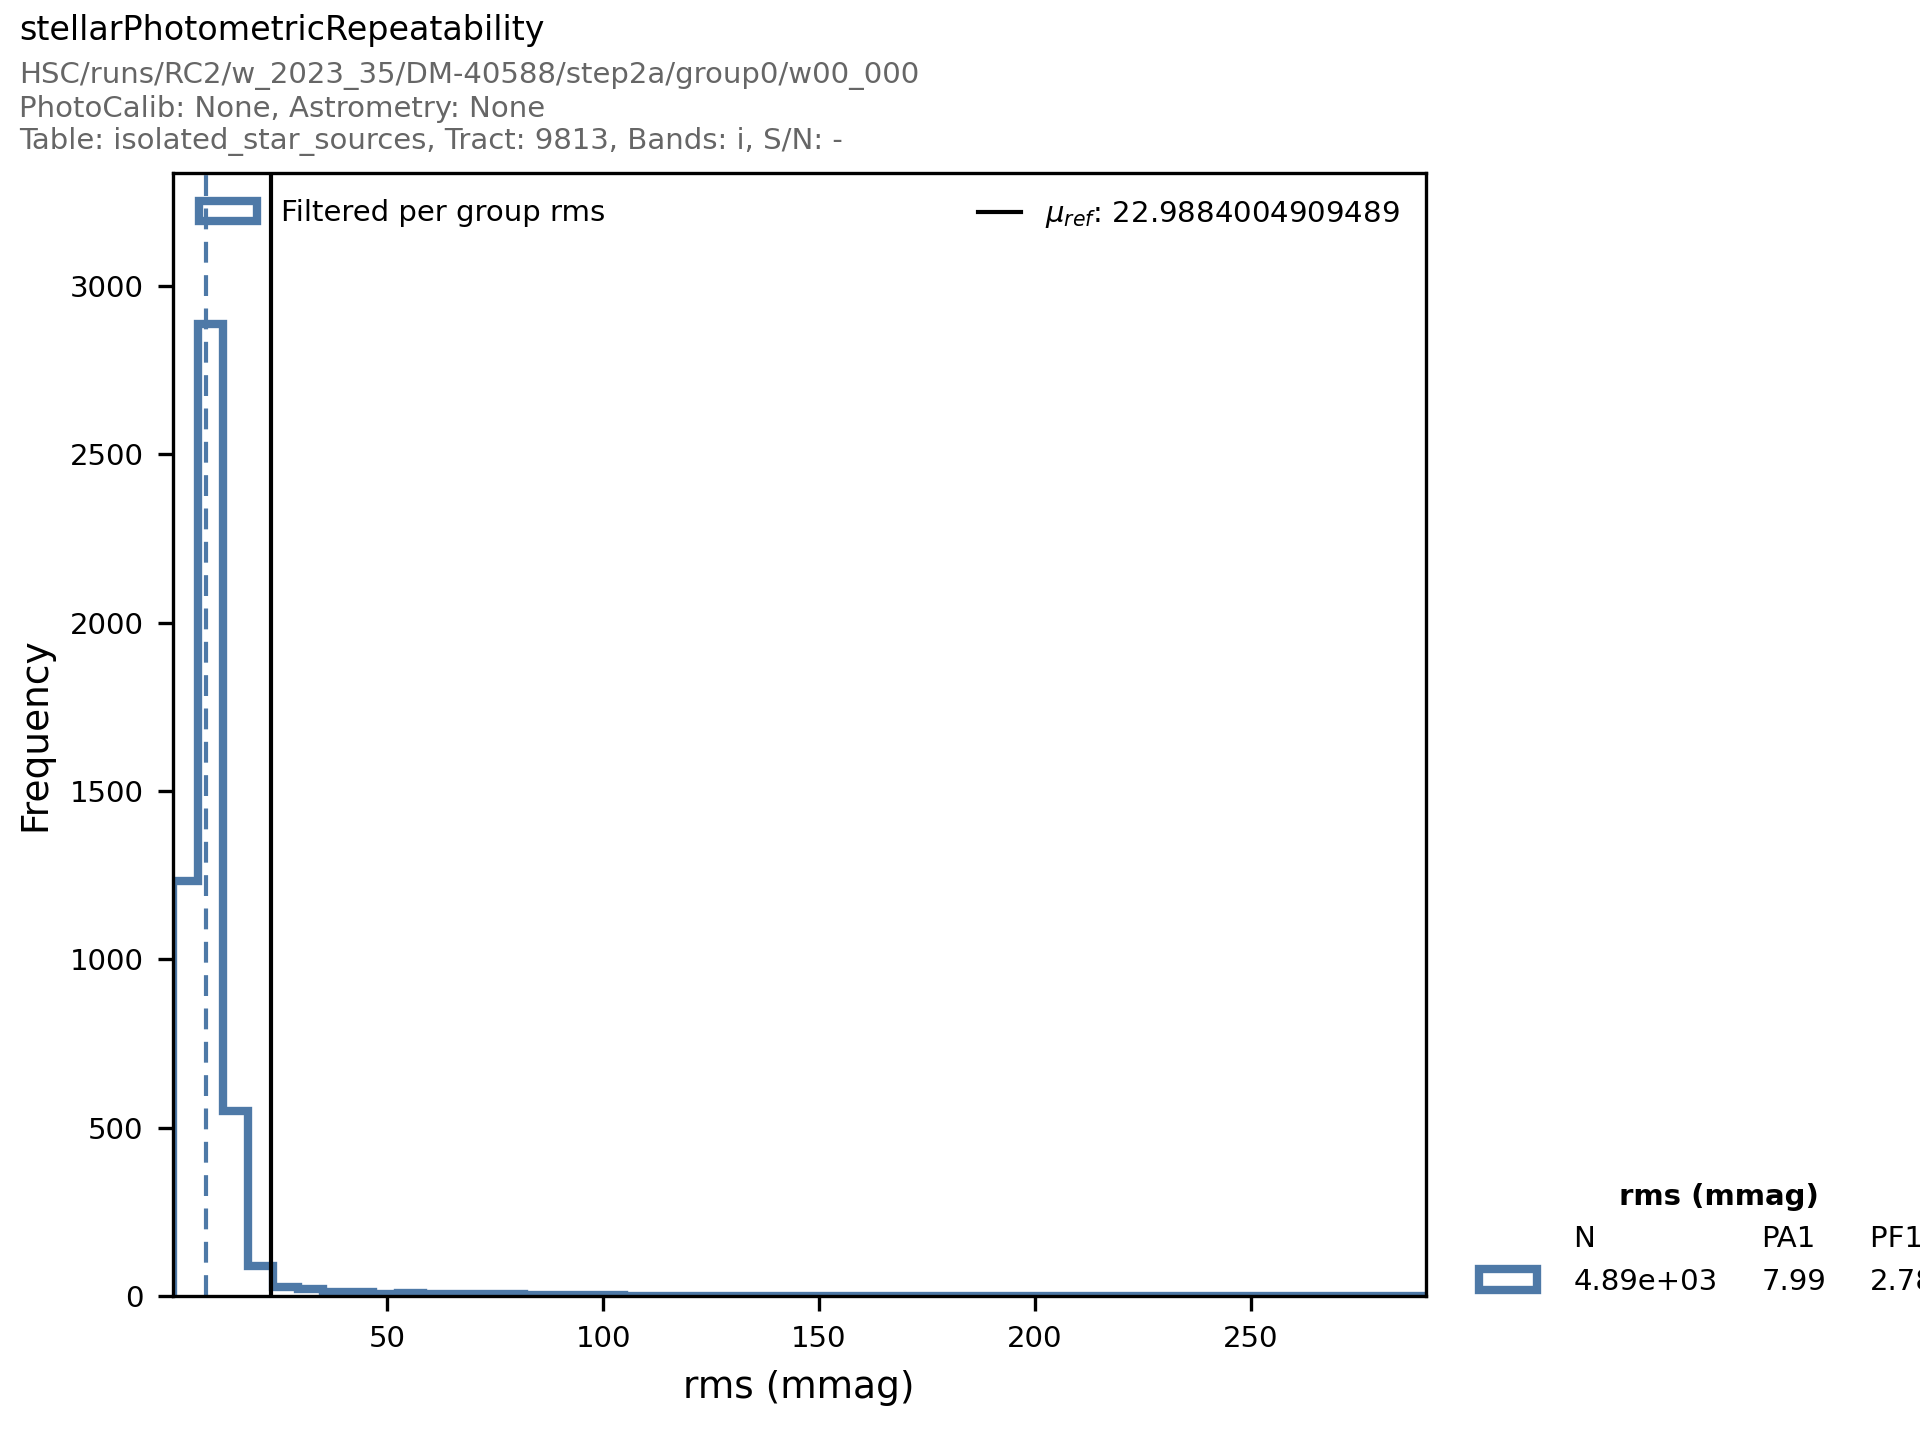
\includegraphics[width=4.66667in, ]{jira_imgs/4828.png}

}
\begin{tabular}{p{4cm}p{12cm}}
\toprule
Step LVV-E2970-5 & Step Execution Status: \textbf{ Pass } \\ \hline
\end{tabular}
 Description \\
{\footnotesize
Change the value of the PA2 threshold in the pipeline yaml for
analysis\_tools, then rerun analysis\_tools

}
\hdashrule[0.5ex]{\textwidth}{1pt}{3mm}
  Expected Result \\
{\footnotesize

}
\hdashrule[0.5ex]{\textwidth}{1pt}{3mm}
  Actual Result \\
{\footnotesize
Changed the following line in matchedVisitQualityCore\_changePA2.yaml:\\
atools.stellarPhotometricRepeatability.PA2Value: 25.0\\
\strut \\
then executed:\\
pipetask -\/-long-log run -j 2 -b /repo/main -\/-register-dataset-types
-p matchedVisitQualityCore\_changePA2.yaml -d "band in
(\textquotesingle g\textquotesingle, \textquotesingle r\textquotesingle,
\textquotesingle i\textquotesingle) AND tract=9813 AND
skymap=\textquotesingle hsc\_rings\_v1\textquotesingle{} AND
instrument=\textquotesingle HSC\textquotesingle" -\/-output
u/jcarlin/pa2\_25 -i HSC/runs/RC2/w\_2023\_35/DM-40588 -\/-instrument
lsst.obs.subaru.HyperSuprimeCam 2\textgreater\&1 \textbar{} tee
w35\_2023\_tract9813\_pa2\_25.txt

}
\begin{tabular}{p{4cm}p{12cm}}
\toprule
Step LVV-E2970-6 & Step Execution Status: \textbf{ Pass } \\ \hline
\end{tabular}
 Description \\
{\footnotesize
Confirm that the new PA2 threshold has been applied when computing PF1.

}
\hdashrule[0.5ex]{\textwidth}{1pt}{3mm}
  Expected Result \\
{\footnotesize
A JSON file (and/or a report generated from that JSON file)
demonstrating that PF1 has been calculated (and that it used the
requested threshold value of PA2gri).

}
\hdashrule[0.5ex]{\textwidth}{1pt}{3mm}
  Actual Result \\
{\footnotesize
Open a python terminal to check the results:\\
\strut \\
\textgreater\textgreater\textgreater{} from lsst.daf.butler import
Butler\\
\textgreater\textgreater\textgreater{}
repo=\textquotesingle/repo/main\textquotesingle{}\\
\textgreater\textgreater\textgreater{}
collection=\textquotesingle u/jcarlin/pa2\_25\textquotesingle{}\\
\textgreater\textgreater\textgreater{} butler = Butler(repo,
collections=collection)\\
\textgreater\textgreater\textgreater{} dataId =
\{\textquotesingle tract\textquotesingle:9813,
\textquotesingle instrument\textquotesingle:\textquotesingle HSC\textquotesingle,
\textquotesingle skymap\textquotesingle:\textquotesingle hsc\_rings\_v1\textquotesingle\}\\
\textgreater\textgreater\textgreater{} metrics =
butler.get(\textquotesingle matchedVisitCore\_metrics\textquotesingle,
dataId=dataId)\\
\textgreater\textgreater\textgreater{} for m in
metrics{[}\textquotesingle stellarPhotometricRepeatability\textquotesingle{]}:\\
... ~ ~~print(m)\\
...~\\
g\_stellarPhotRepeatStdev: 6.979476571776661 mmag\\
g\_stellarPhotRepeatOutlierFraction: 3.1032885595182953 \%\\
g\_ct: 2159.0 ct\\
r\_stellarPhotRepeatStdev: 8.902557135179485 mmag\\
r\_stellarPhotRepeatOutlierFraction: 3.07610713338637 \%\\
r\_ct: 3771.0 ct\\
i\_stellarPhotRepeatStdev: 7.9884004909489015 mmag\\
i\_stellarPhotRepeatOutlierFraction: 1.859799713876967 \%\\
i\_ct: 4893.0 ct\\
z\_stellarPhotRepeatStdev: nan mmag\\
z\_stellarPhotRepeatOutlierFraction: nan \%\\
z\_ct: 0.0 ct\\
y\_stellarPhotRepeatStdev: nan mmag\\
y\_stellarPhotRepeatOutlierFraction: nan \%\\
y\_ct: 0.0 ct\\
\textgreater\textgreater\textgreater{} metrics\_config =
butler.get(\textquotesingle analyzeMatchedVisitCore\_config\textquotesingle,
dataId=dataId)\\
\textgreater\textgreater\textgreater{} config\_dict =
metrics\_config.toDict()\\
\textgreater\textgreater\textgreater{}
config\_dict{[}\textquotesingle atools\textquotesingle{]}{[}\textquotesingle stellarPhotometricRepeatability\textquotesingle{]}{[}\textquotesingle process\textquotesingle{]}{[}\textquotesingle calculateActions\textquotesingle{]}{[}\textquotesingle photRepeatOutlier\textquotesingle{]}\\
\{\textquotesingle op\textquotesingle:
\textquotesingle ge\textquotesingle,
\textquotesingle threshold\textquotesingle: 25.0,
\textquotesingle vectorKey\textquotesingle:
\textquotesingle perGroupStdevFiltered\textquotesingle,
\textquotesingle percent\textquotesingle: True,
\textquotesingle relative\_to\_median\textquotesingle: True\}\\
\strut \\
We can see from both the butler artifacts seen above, and the figure
below, that the threshold PA2 has been set to 25.0 mmag from the
measured PA1 value, as requested.\\
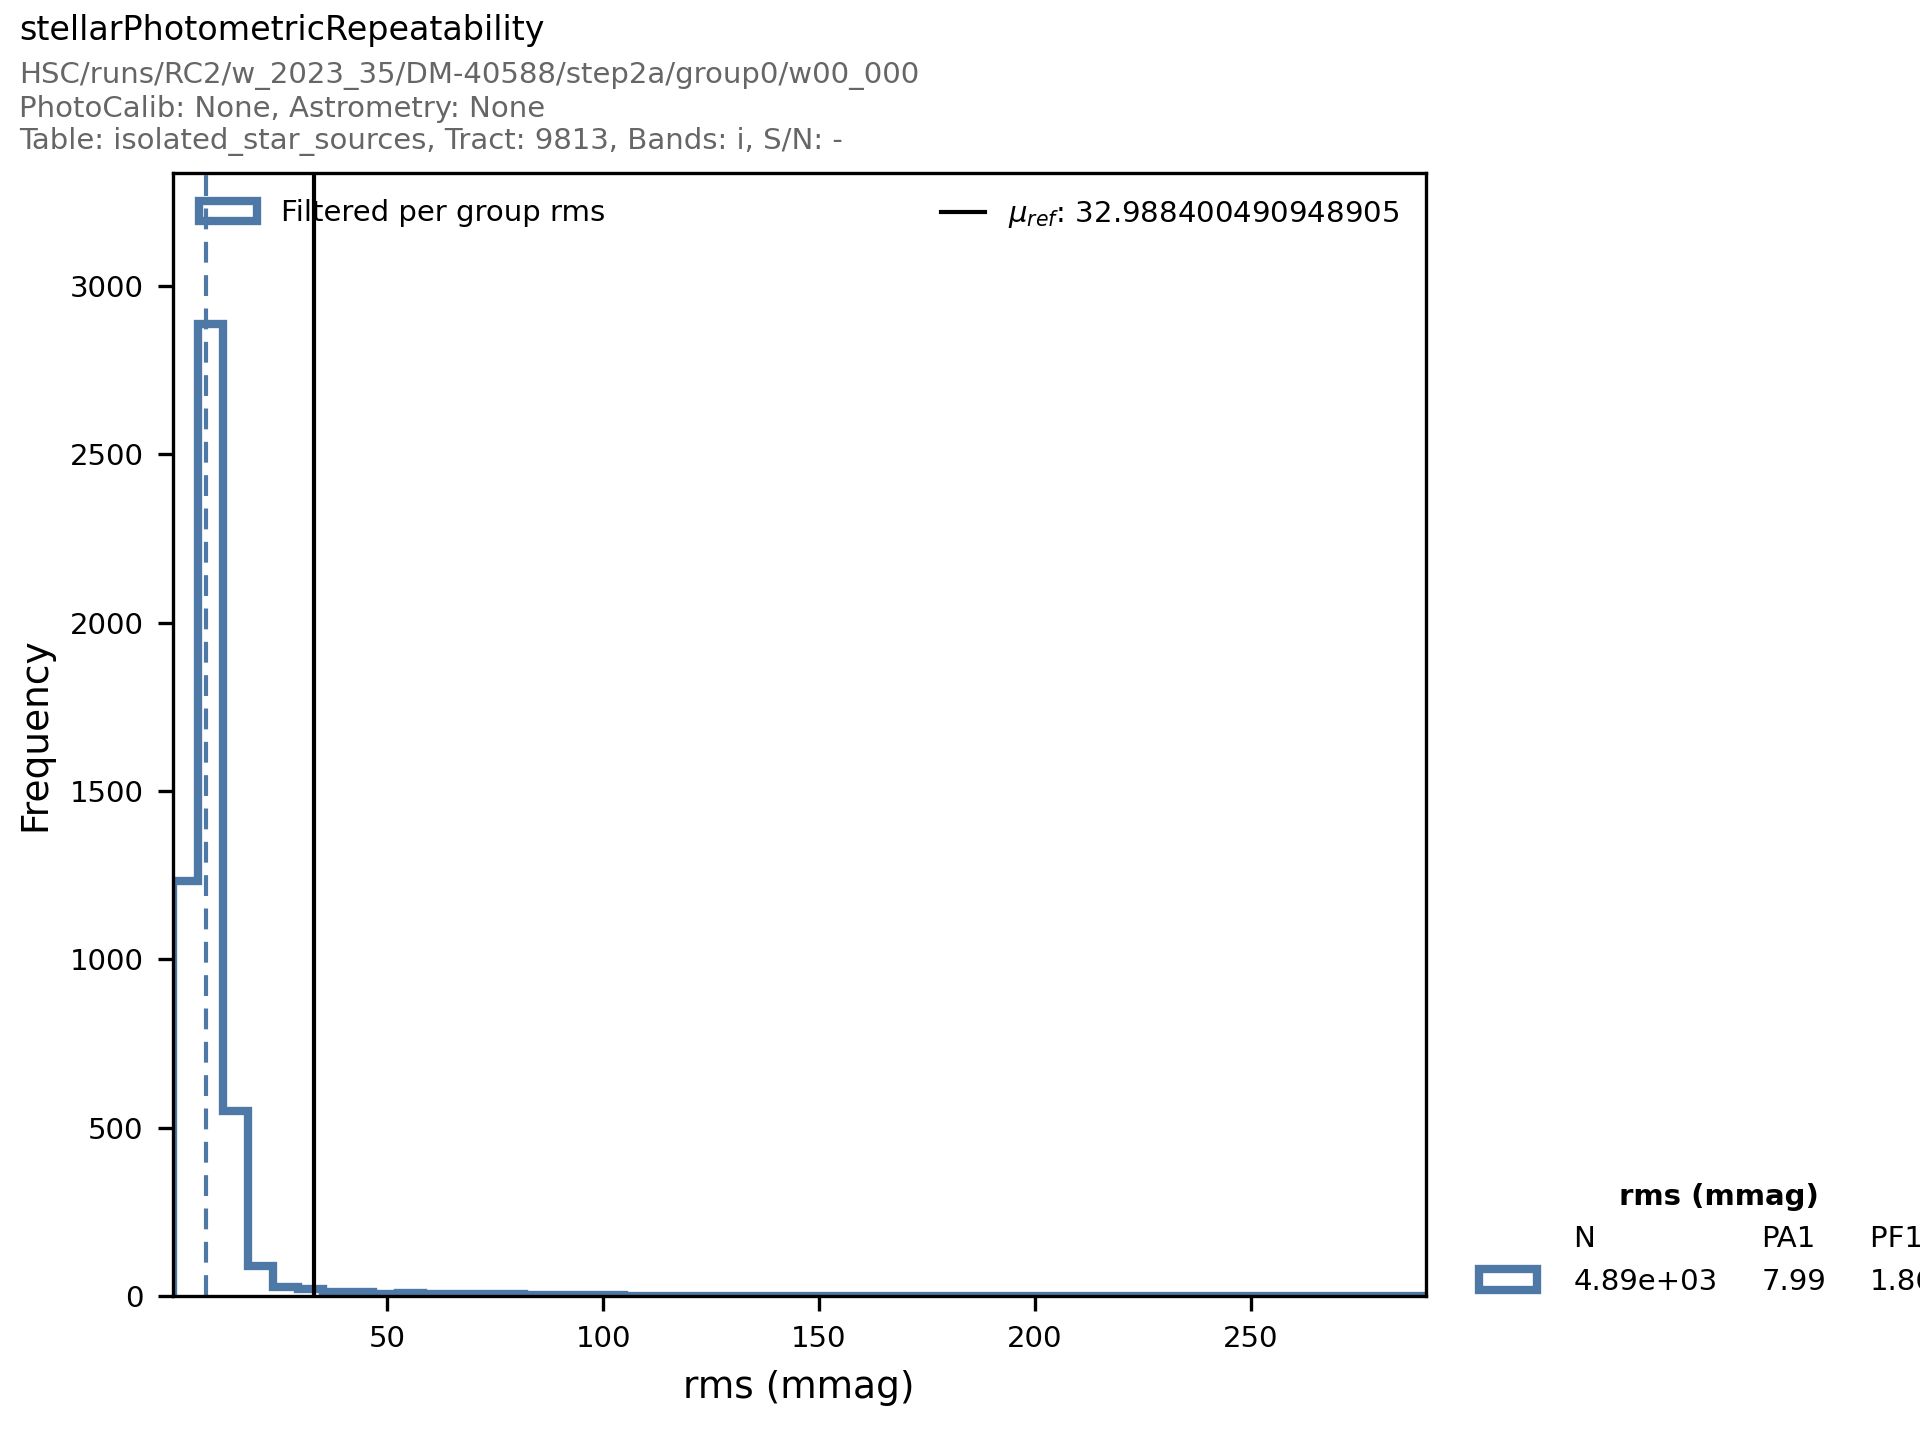
\includegraphics[width=4.26042in, ]{jira_imgs/4829.png}We
have thus demonstrated that the repeatability outlier limit PA2 can be
applied for the gri bands.

}

\paragraph{ LVV-T1758 - Verify that the repeatability outlier limit for isolated bright
non-saturated point sources in the u, z, and y filters (PA2uzy) can be
applied. }\mbox{}\\

Version \textbf{1}.
Status \textbf{Approved}.
Open  \href{https://jira.lsstcorp.org/secure/Tests.jspa#/testCase/LVV-T1758}{\textit{ LVV-T1758 } }
test case in Jira.

Verify that the DM system has provided the code to apply the
repeatability outlier limit for isolated bright non-saturated point
sources in the u, z, and y filters(PA2uzy) to computed values of the PF1
metric.

\textbf{ Preconditions}:\\


Execution status: {\bf  }

Final comment:\\



Detailed steps results LVV-C260-LVV-T1758 LVV-E2971-3366:\\
{\bf Note:} Steps "Not Executed" and with No Result are not shown in this report.\\
\begin{tabular}{p{4cm}p{12cm}}
\toprule
Step LVV-E2971-1 & Step Execution Status: \textbf{ Pass } \\ \hline
\end{tabular}
 Description \\
{\footnotesize
Identify a dataset containing at least one field in each of the u, z,
and y filters with multiple overlapping visits.

}
\hdashrule[0.5ex]{\textwidth}{1pt}{3mm}
  Expected Result \\
{\footnotesize
A dataset that has been ingested into a Butler repository.

}
\hdashrule[0.5ex]{\textwidth}{1pt}{3mm}
  Actual Result \\
{\footnotesize
For this test we use the most recent reprocessing of the Subaru+HSC RC2
dataset. The data were processed with the w\_2023\_35 pipelines.

}
\begin{tabular}{p{4cm}p{12cm}}
\toprule
Step LVV-E2971-2 & Step Execution Status: \textbf{ Pass } \\ \hline
\end{tabular}
 Description \\
{\footnotesize
The `path` that you will use depends on where you are running the
science pipelines. Options:\\
\strut \\

\begin{itemize}
\tightlist
\item
  local (newinstall.sh - based
  install):{[}path\_to\_installation{]}/loadLSST.bash
\item
  development cluster ("lsst-dev"): /software/lsstsw/stack/loadLSST.bash
\item
  LSP Notebook aspect (from a terminal):
  /opt/lsst/software/stack/loadLSST.bash
\end{itemize}

\hfill\break
From the command line, execute the commands below in the example code:\\
\strut \\

}
\hdashrule[0.5ex]{\textwidth}{1pt}{3mm}
  Example Code \\
{\footnotesize
source `path`\\
setup lsst\_distrib

}
\hdashrule[0.5ex]{\textwidth}{1pt}{3mm}
  Expected Result \\
{\footnotesize
Science pipeline software is available for use. If additional packages
are needed (for example, \textquotesingle obs\textquotesingle{} packages
such as `obs\_subaru`), then additional `setup` commands will be
necessary.\\
\strut \\
To check versions in use, type:\\
eups list -s

}
\hdashrule[0.5ex]{\textwidth}{1pt}{3mm}
  Actual Result \\
{\footnotesize
Current weekly stack initialized:\\
\textbf{lsst\_distrib} g4213664e8e+7835acb1bb w\_latest current
w\_2023\_40 setup

}
\begin{tabular}{p{4cm}p{12cm}}
\toprule
Step LVV-E2971-3 & Step Execution Status: \textbf{ Pass } \\ \hline
\end{tabular}
 Description \\
{\footnotesize
Execute `analysis\_tools` on a repository containing processed data.
Identify the path to the data, which we will call
\textquotesingle DATA/path\textquotesingle, then execute something
similar to the following (with paths, datasets, and flags replaced or
additionally specified as needed):

}
\hdashrule[0.5ex]{\textwidth}{1pt}{3mm}
  Example Code \\
{\footnotesize
pipetask -\/-long-log run -j 2 -b DATA/path/butler.yaml
-\/-register-dataset-types -p
\$ANALYSIS\_TOOLS\_DIR/pipelines/matchedVisitQualityCore.yaml -d "band
in (\textquotesingle g\textquotesingle,
\textquotesingle r\textquotesingle, \textquotesingle i\textquotesingle)
AND tract=9813 AND
skymap=\textquotesingle hsc\_rings\_v1\textquotesingle{} AND
instrument=\textquotesingle HSC\textquotesingle" -\/-output
u/username/atools\_metrics -i HSC/runs/RC2/w\_2023\_36 -\/-instrument
lsst.obs.subaru.HyperSuprimeCam 2\textgreater\&1 \textbar{} tee
w36\_2023\_tract9813\_atools.txt

}
\hdashrule[0.5ex]{\textwidth}{1pt}{3mm}
  Expected Result \\
{\footnotesize
The output collection (in this case, "u/username/atools\_metrics")
containing metric measurements and any associated extras and metadata is
available via the butler.

}
\hdashrule[0.5ex]{\textwidth}{1pt}{3mm}
  Actual Result \\
{\footnotesize
Changed the value of PA2 in matchedVisitQualityCore\_changePA2.yaml to
15.0:\\
atools.stellarPhotometricRepeatability.PA2Value: 15.0\\
\strut \\
Then, executed the pipeline as follows:\\
pipetask -\/-long-log run -j 2 -b /repo/main -\/-register-dataset-types
-p matchedVisitQualityCore\_changePA2.yaml -d "band in
(\textquotesingle z\textquotesingle, \textquotesingle y\textquotesingle)
AND tract=9813 AND
skymap=\textquotesingle hsc\_rings\_v1\textquotesingle{} AND
instrument=\textquotesingle HSC\textquotesingle" -\/-output
u/jcarlin/pa2\_15\_zy -i HSC/runs/RC2/w\_2023\_35/DM-40588
-\/-instrument lsst.obs.subaru.HyperSuprimeCam 2\textgreater\&1
\textbar{} tee w35\_2023\_tract9813\_zy\_pa2\_15.txt\\
\strut \\

}
\begin{tabular}{p{4cm}p{12cm}}
\toprule
Step LVV-E2971-4 & Step Execution Status: \textbf{ Pass } \\ \hline
\end{tabular}
 Description \\
{\footnotesize
Confirm that the PA2uzy threshold has been applied to the assessment of
the computed values of PF1 for filters u,z,y.

}
\hdashrule[0.5ex]{\textwidth}{1pt}{3mm}
  Expected Result \\
{\footnotesize
A JSON file (and/or a report generated from that JSON file)
demonstrating that PF1 has been calculated (and that it used the
requested PA2uzy threshold).

}
\hdashrule[0.5ex]{\textwidth}{1pt}{3mm}
  Actual Result \\
{\footnotesize
Examine the results in a python terminal:\\
\strut \\
\textgreater\textgreater\textgreater{} from lsst.daf.butler import
Butler\\
\textgreater\textgreater\textgreater{}
repo=\textquotesingle/repo/main\textquotesingle{}\\
\textgreater\textgreater\textgreater{}
collection=\textquotesingle u/jcarlin/pa2\_15\_zy\textquotesingle{}\\
\textgreater\textgreater\textgreater{} butler = Butler(repo,
collections=collection)\\
\textgreater\textgreater\textgreater{} dataId =
\{\textquotesingle tract\textquotesingle:9813,
\textquotesingle instrument\textquotesingle:\textquotesingle HSC\textquotesingle,
\textquotesingle skymap\textquotesingle:\textquotesingle hsc\_rings\_v1\textquotesingle\}\\
\textgreater\textgreater\textgreater{} metrics =
butler.get(\textquotesingle matchedVisitCore\_metrics\textquotesingle,
dataId=dataId)\\
\textgreater\textgreater\textgreater{} for m in
metrics{[}\textquotesingle stellarPhotometricRepeatability\textquotesingle{]}:\\
... print(m)\\
...\\
z\_stellarPhotRepeatStdev: 6.924991284071611 mmag\\
z\_stellarPhotRepeatOutlierFraction: 1.9053231192300137 \%\\
z\_ct: 5091.0 ct\\
y\_stellarPhotRepeatStdev: 7.237368762721793 mmag\\
y\_stellarPhotRepeatOutlierFraction: 0.964371818912403 \%\\
y\_ct: 3733.0 ct\\
\textgreater\textgreater\textgreater{} metrics\_config =
butler.get(\textquotesingle analyzeMatchedVisitCore\_config\textquotesingle,
dataId=dataId)\\
\textgreater\textgreater\textgreater{} config\_dict =
metrics\_config.toDict()\\
\textgreater\textgreater\textgreater{}
config\_dict{[}\textquotesingle atools\textquotesingle{]}{[}\textquotesingle stellarPhotometricRepeatability\textquotesingle{]}{[}\textquotesingle process\textquotesingle{]}{[}\textquotesingle calculateActions\textquotesingle{]}{[}\textquotesingle photRepeatOutlier\textquotesingle{]}\\
\{\textquotesingle op\textquotesingle:
\textquotesingle ge\textquotesingle,
\textquotesingle threshold\textquotesingle: 15.0,
\textquotesingle vectorKey\textquotesingle:
\textquotesingle perGroupStdevFiltered\textquotesingle,
\textquotesingle percent\textquotesingle: True,
\textquotesingle relative\_to\_median\textquotesingle: True\}\\
\strut \\
The following figure is output by the pipeline. The threshold (vertical
black line) is set at 15 mmag above the measured PA1 value, as
expected.\\
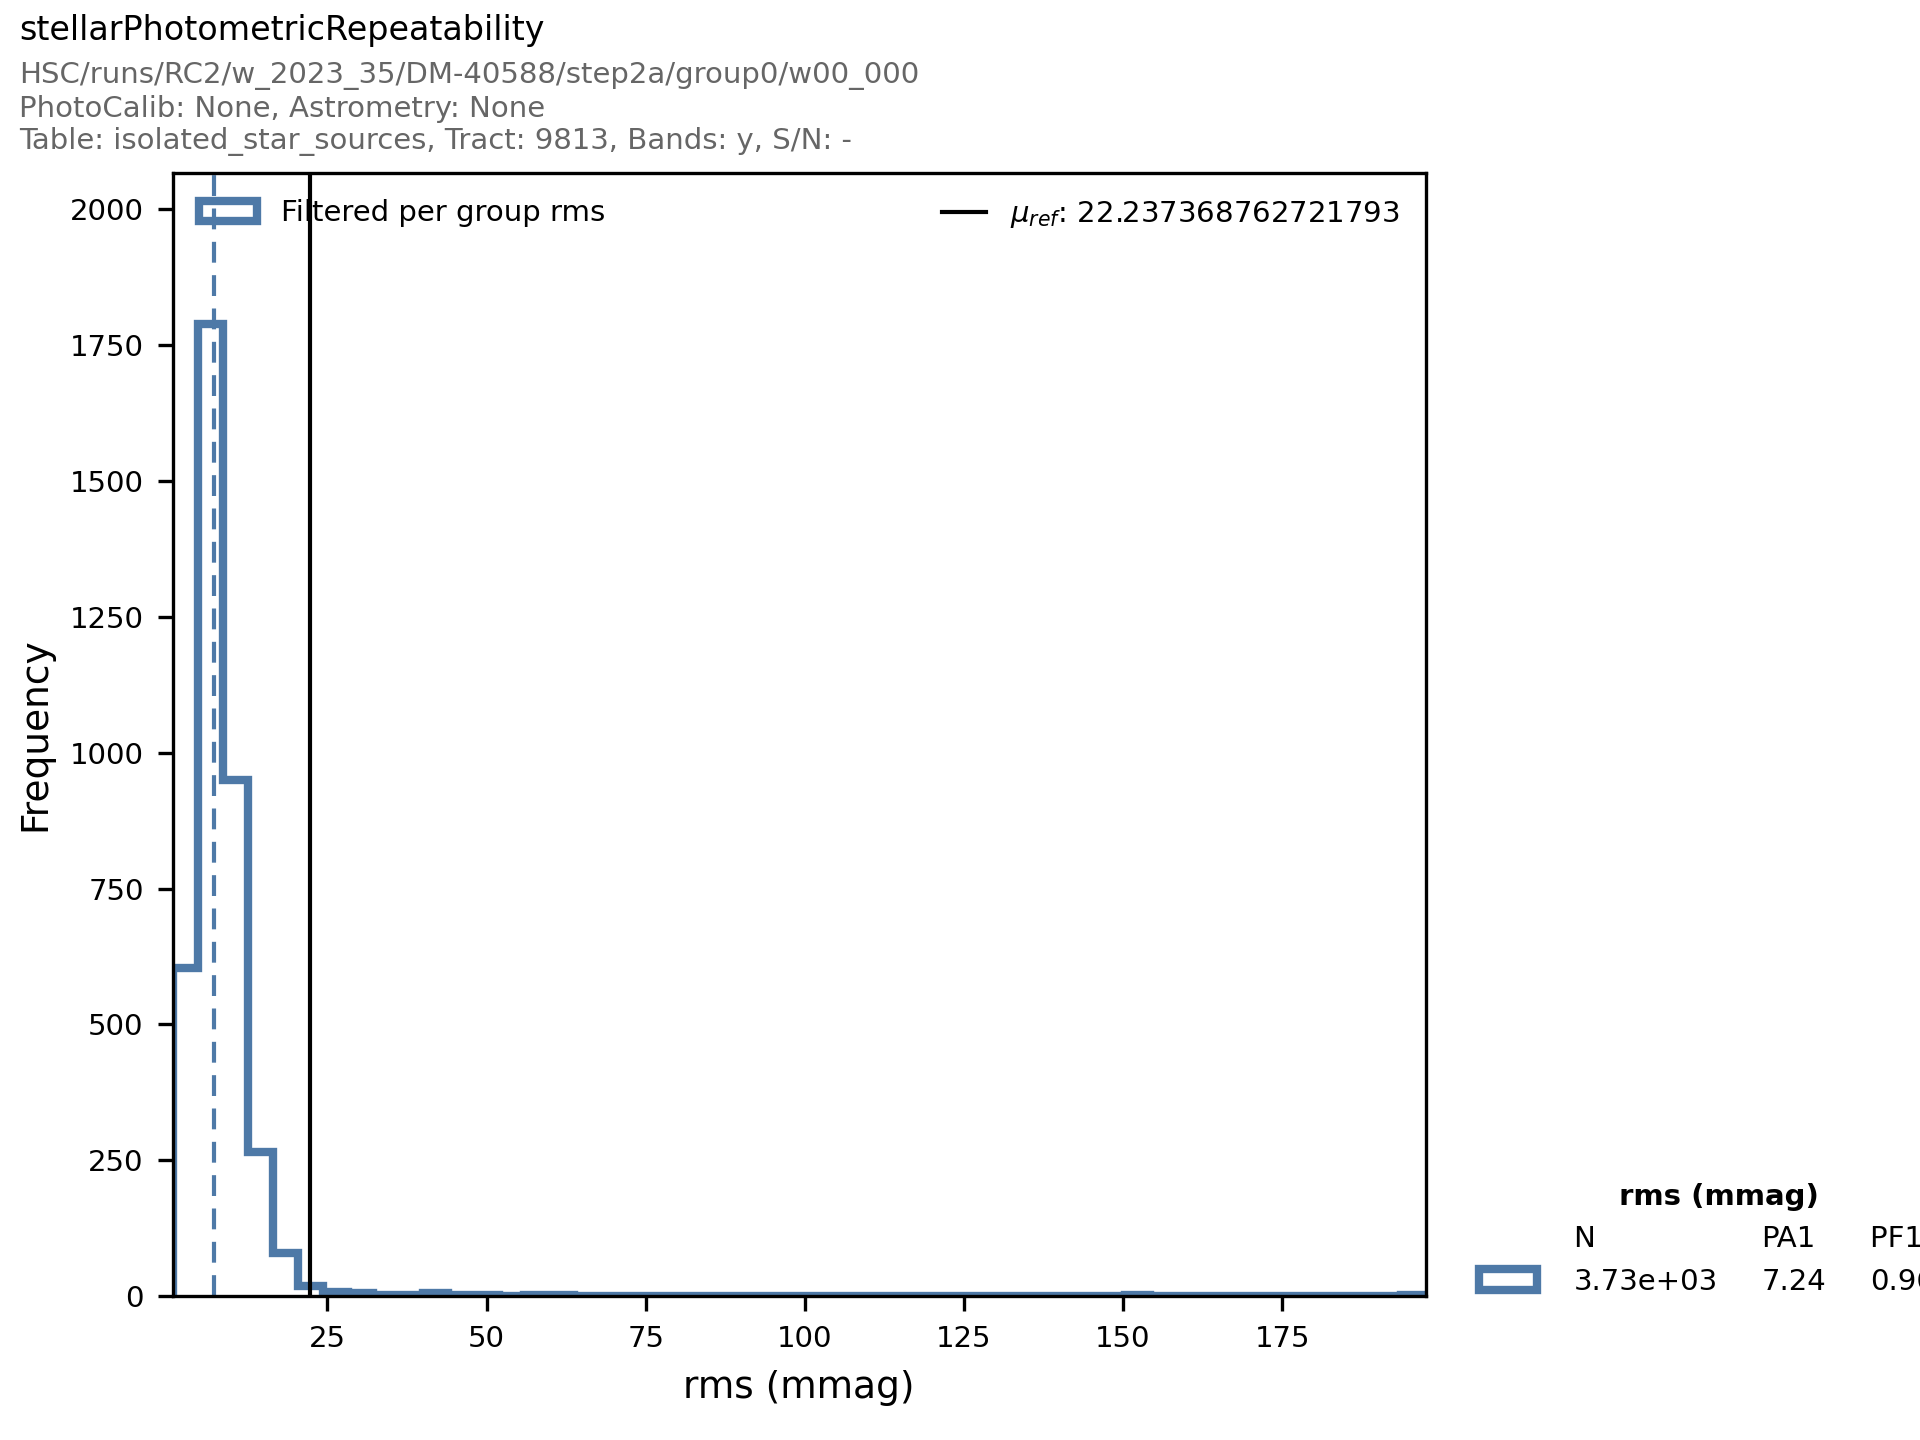
\includegraphics[width=4.33333in, ]{jira_imgs/4830.png}

}
\begin{tabular}{p{4cm}p{12cm}}
\toprule
Step LVV-E2971-5 & Step Execution Status: \textbf{ Pass } \\ \hline
\end{tabular}
 Description \\
{\footnotesize
Change the value of the PA2 threshold in the pipeline yaml for
analysis\_tools, then rerun analysis\_tools

}
\hdashrule[0.5ex]{\textwidth}{1pt}{3mm}
  Expected Result \\
{\footnotesize

}
\hdashrule[0.5ex]{\textwidth}{1pt}{3mm}
  Actual Result \\
{\footnotesize
Changed the following line in matchedVisitQualityCore\_changePA2.yaml:\\
atools.stellarPhotometricRepeatability.PA2Value: 25.0\\
\strut \\
then executed:\\
pipetask -\/-long-log run -j 2 -b /repo/main -\/-register-dataset-types
-p matchedVisitQualityCore\_changePA2.yaml -d "band in
(\textquotesingle z\textquotesingle, \textquotesingle y\textquotesingle)
AND tract=9813 AND
skymap=\textquotesingle hsc\_rings\_v1\textquotesingle{} AND
instrument=\textquotesingle HSC\textquotesingle" -\/-output
u/jcarlin/pa2\_25\_zy -i HSC/runs/RC2/w\_2023\_35/DM-40588
-\/-instrument lsst.obs.subaru.HyperSuprimeCam 2\textgreater\&1
\textbar{} tee w35\_2023\_tract9813\_zy\_pa2\_25.txt\\
\strut \\

}
\begin{tabular}{p{4cm}p{12cm}}
\toprule
Step LVV-E2971-6 & Step Execution Status: \textbf{ Pass } \\ \hline
\end{tabular}
 Description \\
{\footnotesize
Confirm that the new PA2 threshold has been applied when computing PF1.

}
\hdashrule[0.5ex]{\textwidth}{1pt}{3mm}
  Expected Result \\
{\footnotesize
A JSON file (and/or a report generated from that JSON file)
demonstrating that PF1 has been calculated (and that it used the
requested threshold value of PA2gri).

}
\hdashrule[0.5ex]{\textwidth}{1pt}{3mm}
  Actual Result \\
{\footnotesize
\textgreater\textgreater\textgreater{} from lsst.daf.butler import
Butler\\
\textgreater\textgreater\textgreater{}
repo=\textquotesingle/repo/main\textquotesingle{}\\
\textgreater\textgreater\textgreater{}
collection=\textquotesingle u/jcarlin/pa2\_15\_zy\textquotesingle{}\\
\textgreater\textgreater\textgreater{} butler = Butler(repo,
collections=collection)\\
\textgreater\textgreater\textgreater{} dataId =
\{\textquotesingle tract\textquotesingle:9813,
\textquotesingle instrument\textquotesingle:\textquotesingle HSC\textquotesingle,
\textquotesingle skymap\textquotesingle:\textquotesingle hsc\_rings\_v1\textquotesingle\}\\
\textgreater\textgreater\textgreater{} metrics =
butler.get(\textquotesingle matchedVisitCore\_metrics\textquotesingle,
dataId=dataId)\\
\textgreater\textgreater\textgreater{} for m in
metrics{[}\textquotesingle stellarPhotometricRepeatability\textquotesingle{]}:\\
... print(m)\\
...\\
z\_stellarPhotRepeatStdev: 6.924991284071611 mmag\\
z\_stellarPhotRepeatOutlierFraction: 1.9053231192300137 \%\\
z\_ct: 5091.0 ct\\
y\_stellarPhotRepeatStdev: 7.237368762721793 mmag\\
y\_stellarPhotRepeatOutlierFraction: 0.964371818912403 \%\\
y\_ct: 3733.0 ct\\
\textgreater\textgreater\textgreater{} metrics\_config =
butler.get(\textquotesingle analyzeMatchedVisitCore\_config\textquotesingle,
dataId=dataId)\\
\textgreater\textgreater\textgreater{} config\_dict =
metrics\_config.toDict()\\
\textgreater\textgreater\textgreater{}
config\_dict{[}\textquotesingle atools\textquotesingle{]}{[}\textquotesingle stellarPhotometricRepeatability\textquotesingle{]}{[}\textquotesingle process\textquotesingle{]}{[}\textquotesingle calculateActions\textquotesingle{]}{[}\textquotesingle photRepeatOutlier\textquotesingle{]}\\
\{\textquotesingle op\textquotesingle:
\textquotesingle ge\textquotesingle,
\textquotesingle threshold\textquotesingle: 25.0,
\textquotesingle vectorKey\textquotesingle:
\textquotesingle perGroupStdevFiltered\textquotesingle,
\textquotesingle percent\textquotesingle: True,
\textquotesingle relative\_to\_median\textquotesingle: True\}\\
\strut \\
We can see from both the butler artifacts seen above, and the figure
below, that the threshold PA2 has been set to 25.0 mmag from the
measured PA1 value, as requested.\\
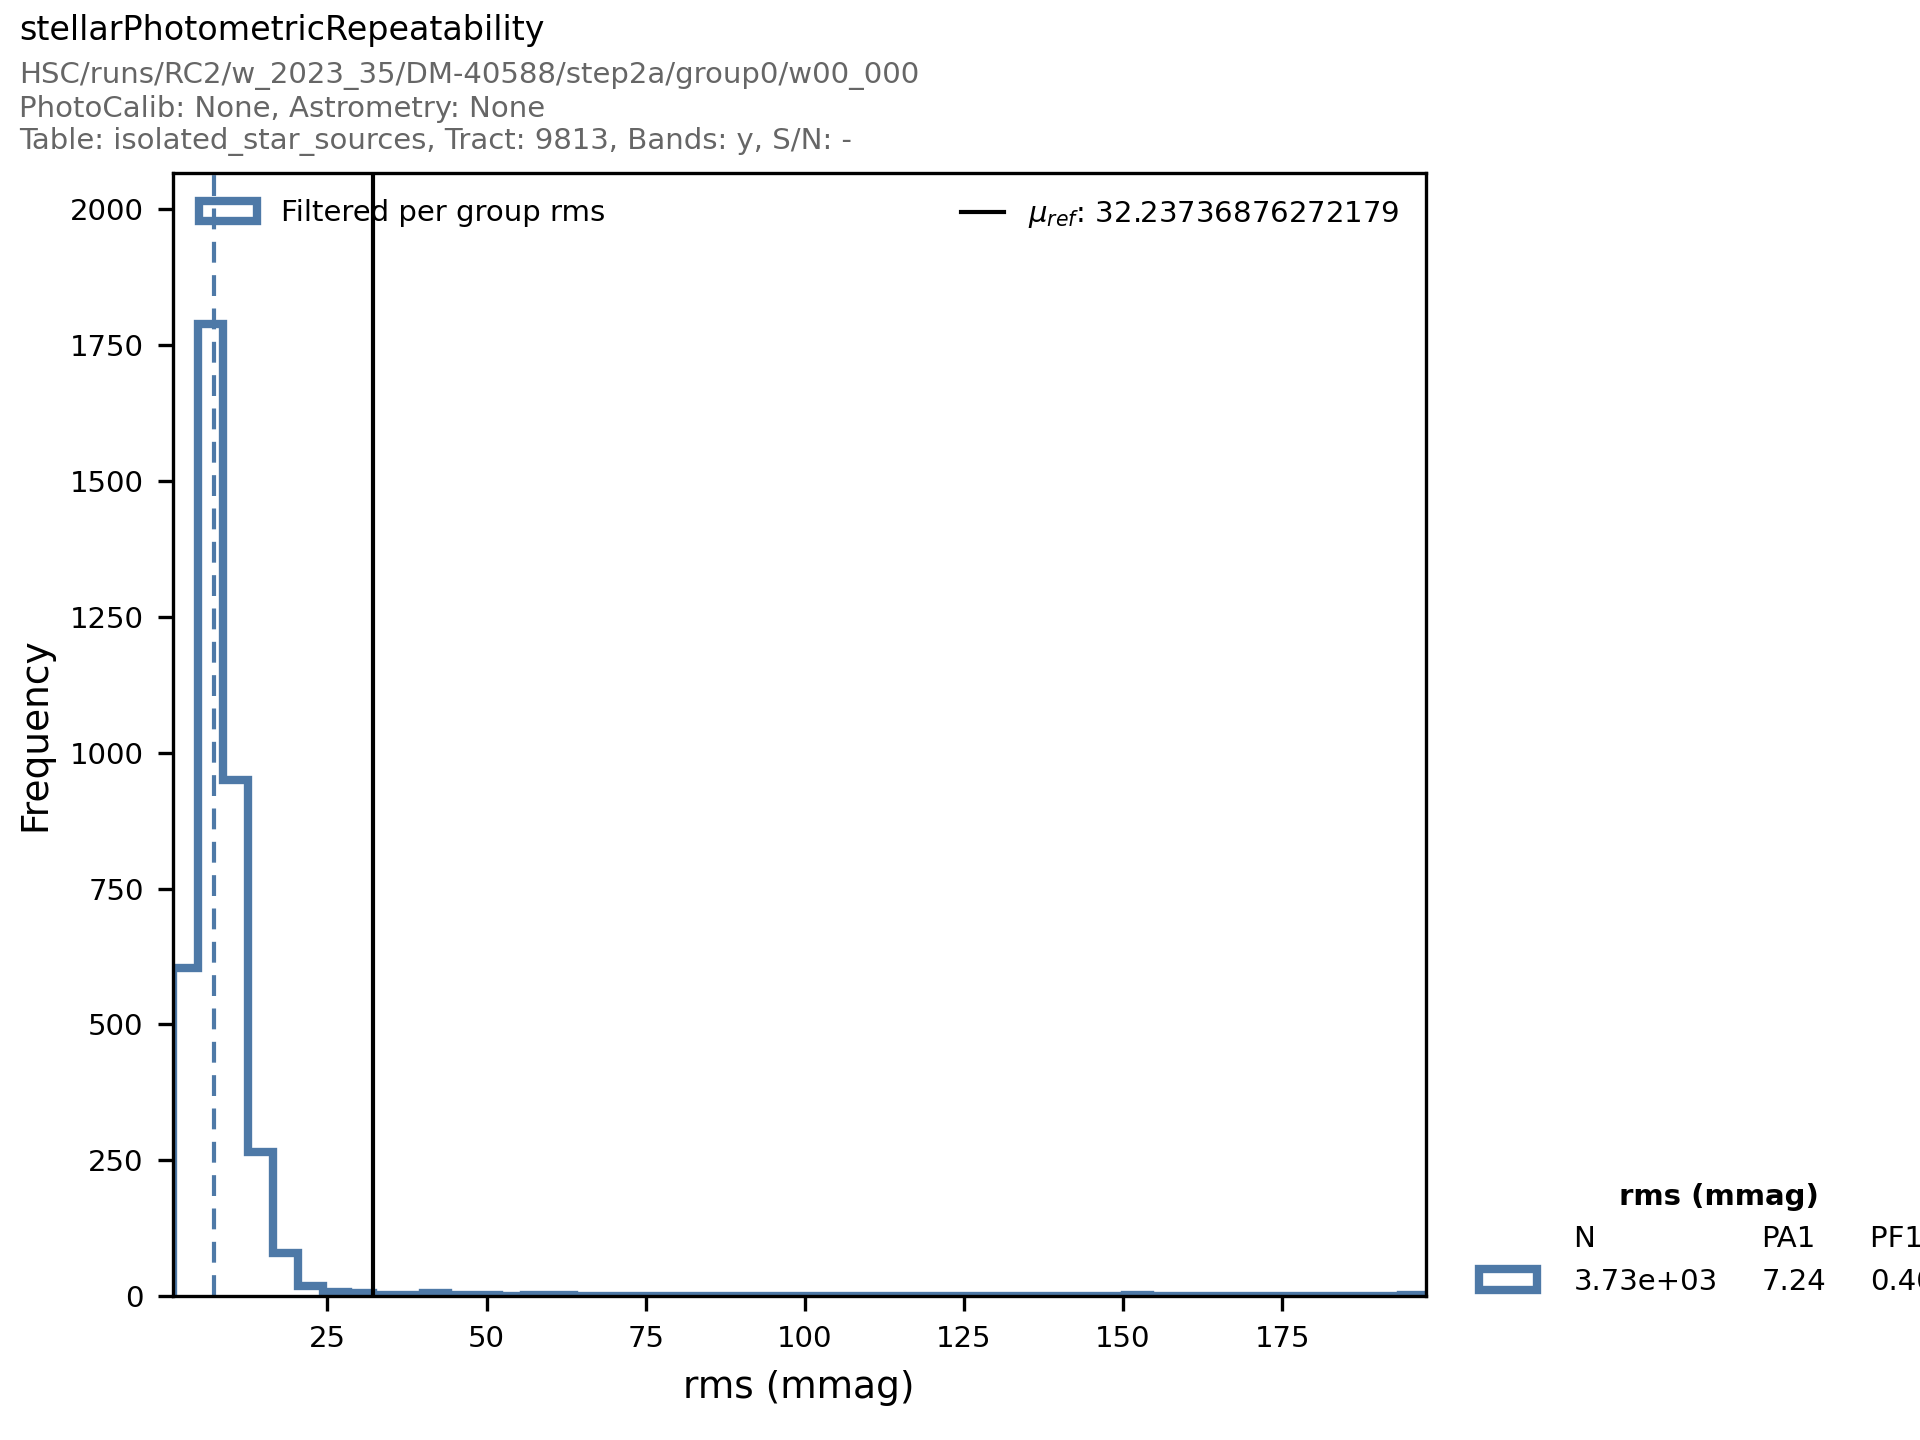
\includegraphics[width=4.48958in, ]{jira_imgs/4831.png}\\
We have thus demonstrated that the repeatability outlier limit PA2 can
be applied for the z and y bands.

}

\paragraph{ LVV-T149 - Verify implementation of Catalog Queries }\mbox{}\\

Version \textbf{1}.
Status \textbf{Approved}.
Open  \href{https://jira.lsstcorp.org/secure/Tests.jspa#/testCase/LVV-T149}{\textit{ LVV-T149 } }
test case in Jira.

Verify that SQL, or a similar structured language, can be used to query
catalogs.

\textbf{ Preconditions}:\\
An operational QSERV database that has been verified via
\href{https://jira.lsstcorp.org/secure/Tests.jspa\#/testCase/LVV-T1085}{LVV-T1085}
and
\href{https://jira.lsstcorp.org/secure/Tests.jspa\#/testCase/LVV-T1086}{LVV-T1086}
and
\href{https://jira.lsstcorp.org/secure/Tests.jspa\#/testCase/LVV-T1087}{LVV-T1087}.

Execution status: {\bf  }

Final comment:\\



Detailed steps results LVV-C260-LVV-T149 LVV-E2972-3367:\\
{\bf Note:} Steps "Not Executed" and with No Result are not shown in this report.\\
\begin{tabular}{p{4cm}p{12cm}}
\toprule
Step LVV-E2972-1 & Step Execution Status: \textbf{ Pass } \\ \hline
\end{tabular}
 Description \\
{\footnotesize
Execute a simple query (for example, the one below) and confirm that it
returns the expected result.

}
\hdashrule[0.5ex]{\textwidth}{1pt}{3mm}
  Example Code \\
{\footnotesize
SELECT * FROM dp02\_dc2\_catalogs.Object as obj WHERE
CONTAINS(POINT(\textquotesingle ICRS\textquotesingle, obj.coord\_ra,
obj.coord\_dec), CIRCLE(\textquotesingle ICRS\textquotesingle, 62.0,
-37.0, 0.10)) = 1

}
\hdashrule[0.5ex]{\textwidth}{1pt}{3mm}
  Expected Result \\
{\footnotesize
A catalog of objects satisfying the specified constraints. The catalog
should contain 26,115 results.

}
\hdashrule[0.5ex]{\textwidth}{1pt}{3mm}
  Actual Result \\
{\footnotesize
The query was executed in the notebook "test\_LVV-T149.ipynb" attached
to this document\textquotesingle s Github repository. The query executed
successfully in the notebook, and returned 26,115 results, as expected.

}
\begin{tabular}{p{4cm}p{12cm}}
\toprule
Step LVV-E2972-2 & Step Execution Status: \textbf{ Pass } \\ \hline
\end{tabular}
 Description \\
{\footnotesize
Repeat the query from all available access routes (e.g., an external VO
client, the Science Platform query tool, and from within the Notebook
Aspect), confirming in each case that the results are as expected.

}
\hdashrule[0.5ex]{\textwidth}{1pt}{3mm}
  Expected Result \\
{\footnotesize

}
\hdashrule[0.5ex]{\textwidth}{1pt}{3mm}
  Actual Result \\
{\footnotesize
The Notebook query was demonstrated in step 1.\\
\strut \\
To query via the API aspect, we use Topcat, entering
"https://data.lsst.cloud/api/tap/" in the "Select TAP service" window as
seen below. (Note that the user has already set up an access token for
Topcat to access the RSP.)\\
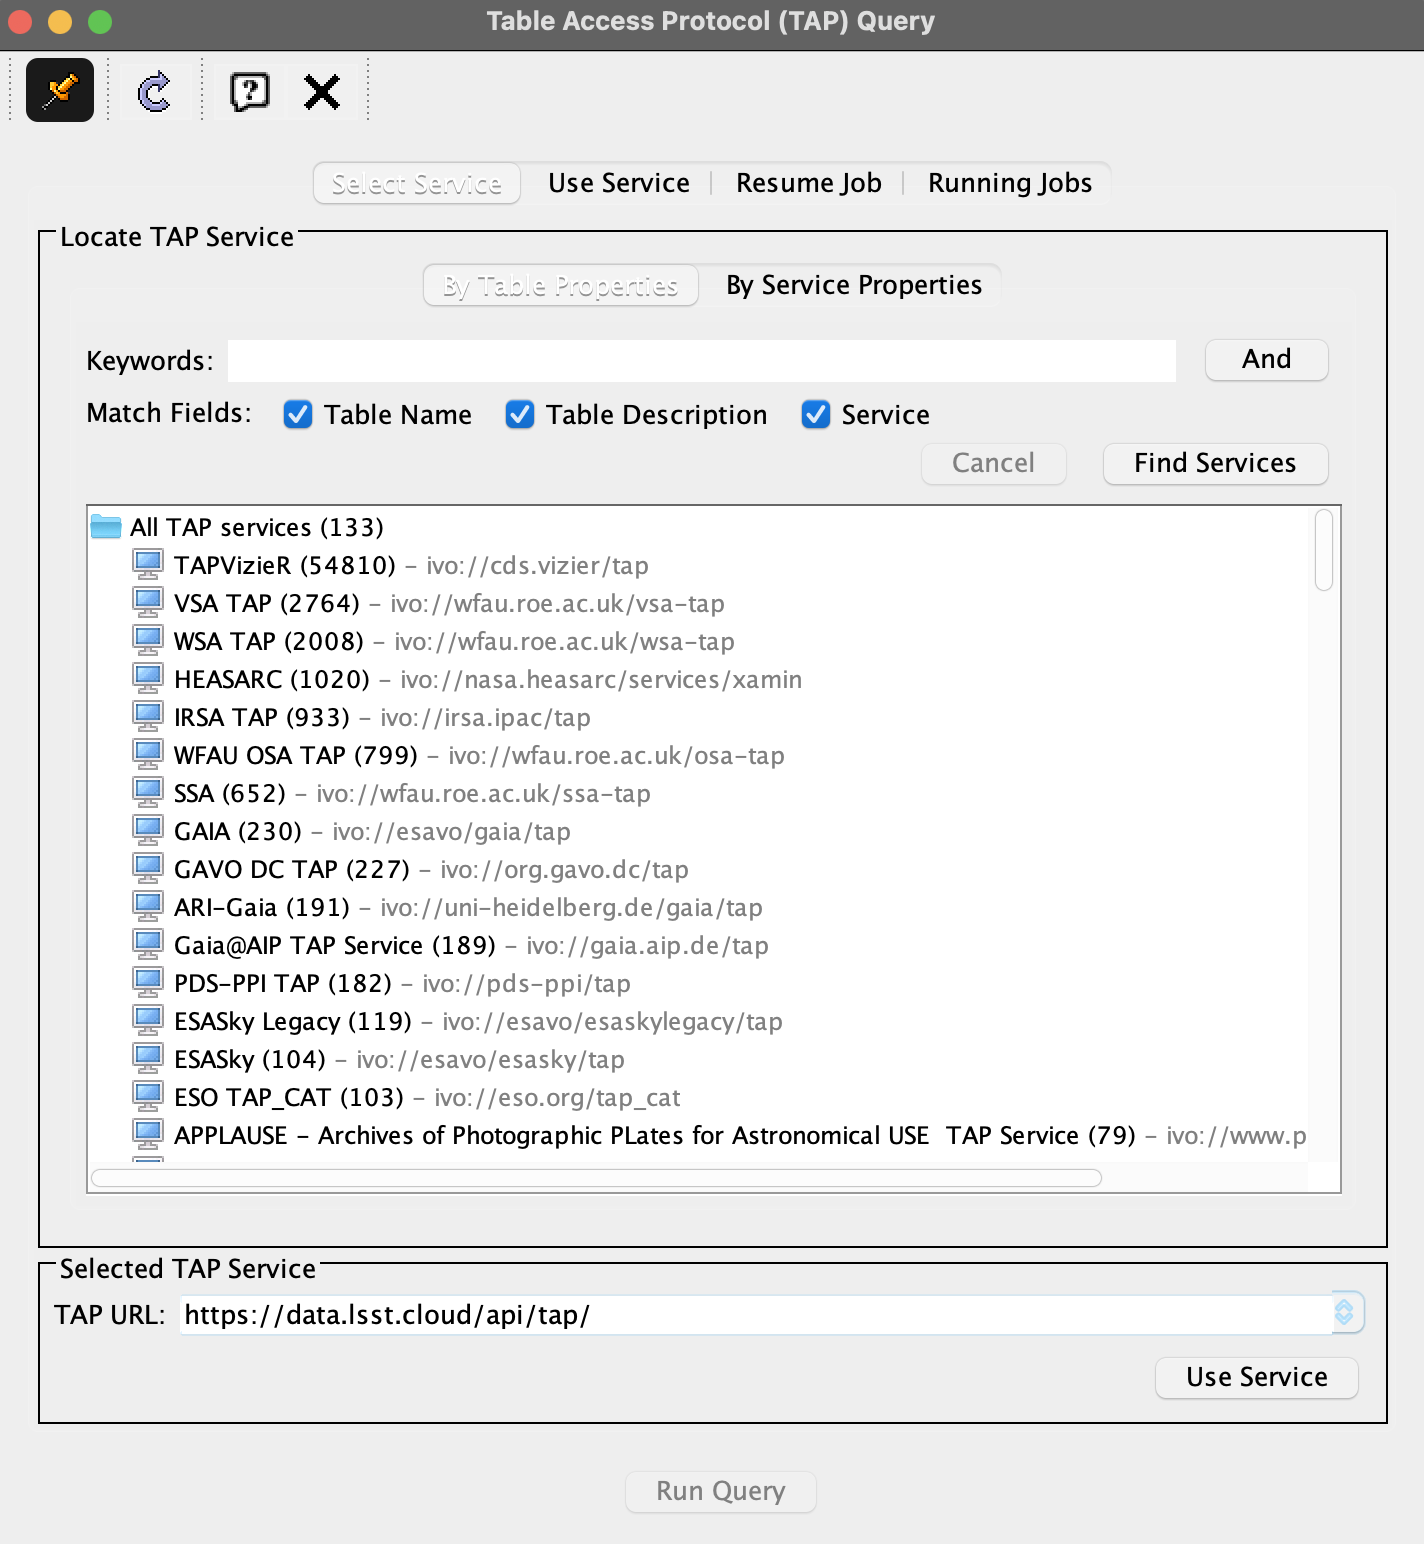
\includegraphics[width=3.79167in, ]{jira_imgs/4609.png}Next
we execute the query from the "Use Service" window as follows:\\
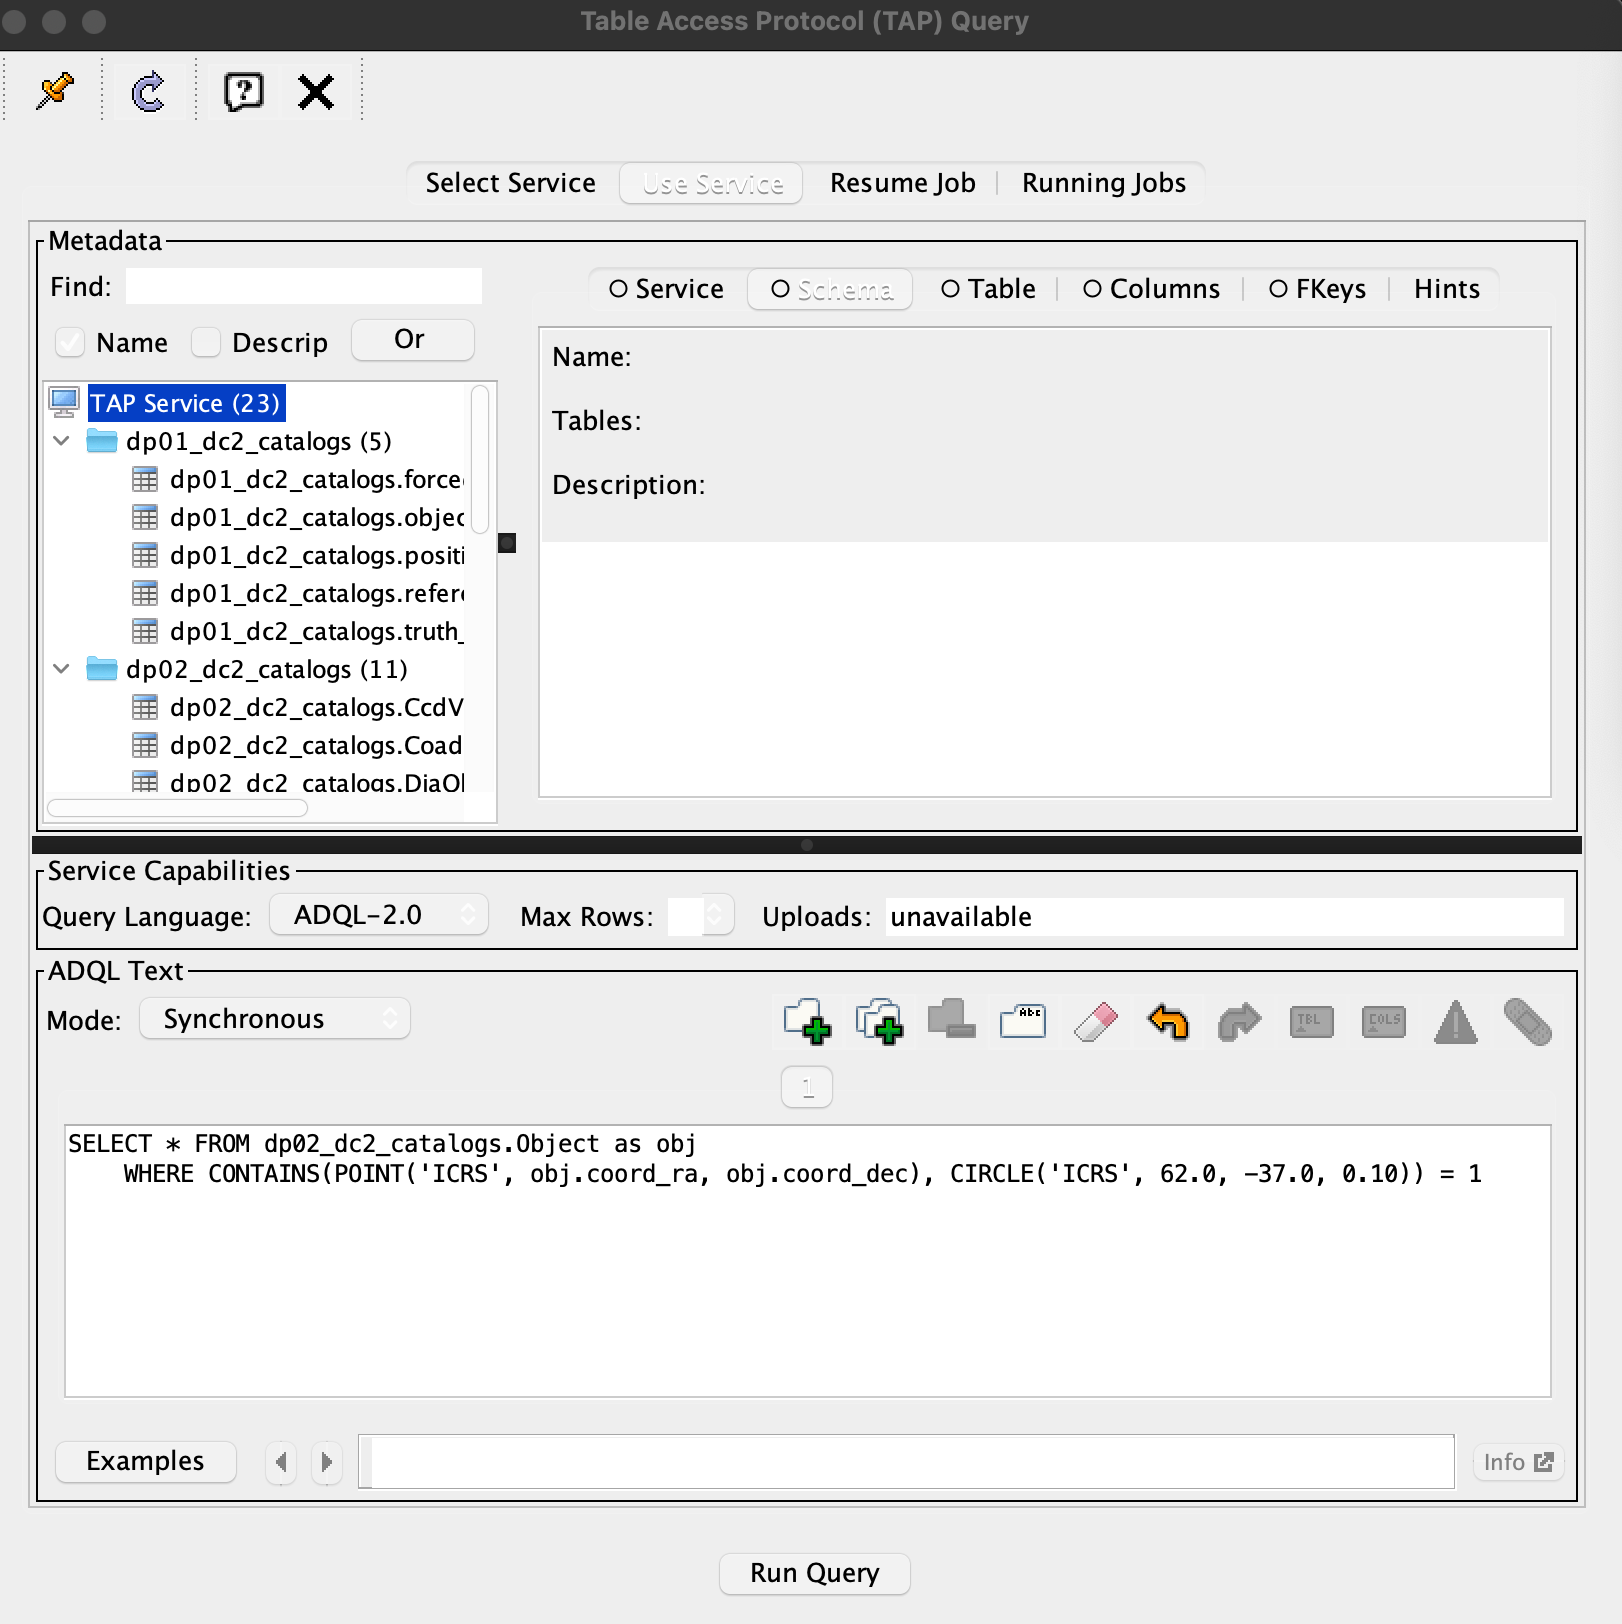
\includegraphics[width=4.41667in, ]{jira_imgs/4610.png}The
following screenshot shows that the query returned 26,115 results (and
991 columns of data), as expected.\\
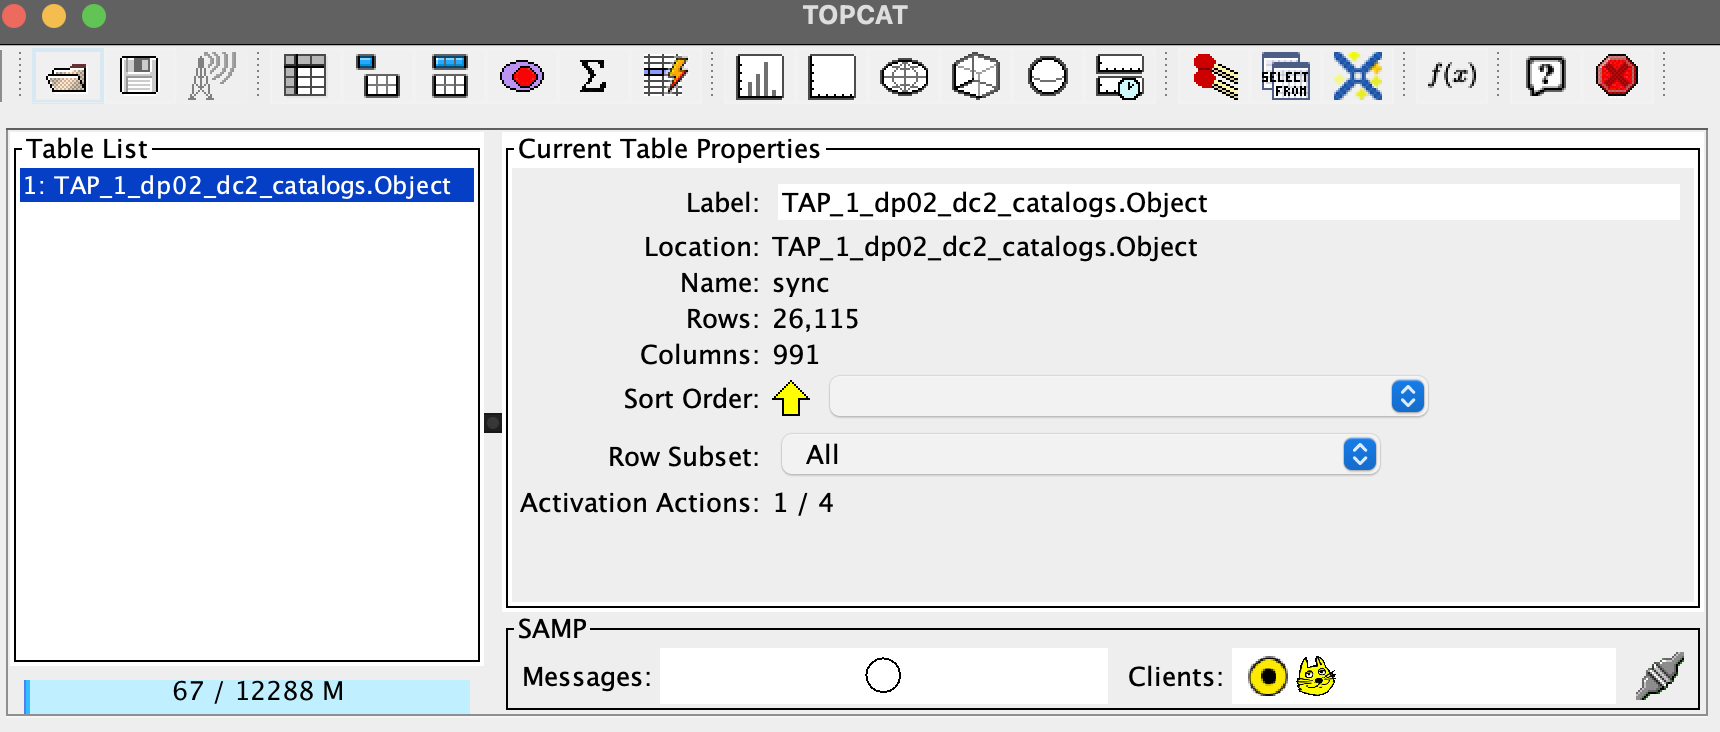
\includegraphics[width=4.78125in, ]{jira_imgs/4611.png}\\
Next we execute the same query from the RSP Portal aspect.\\
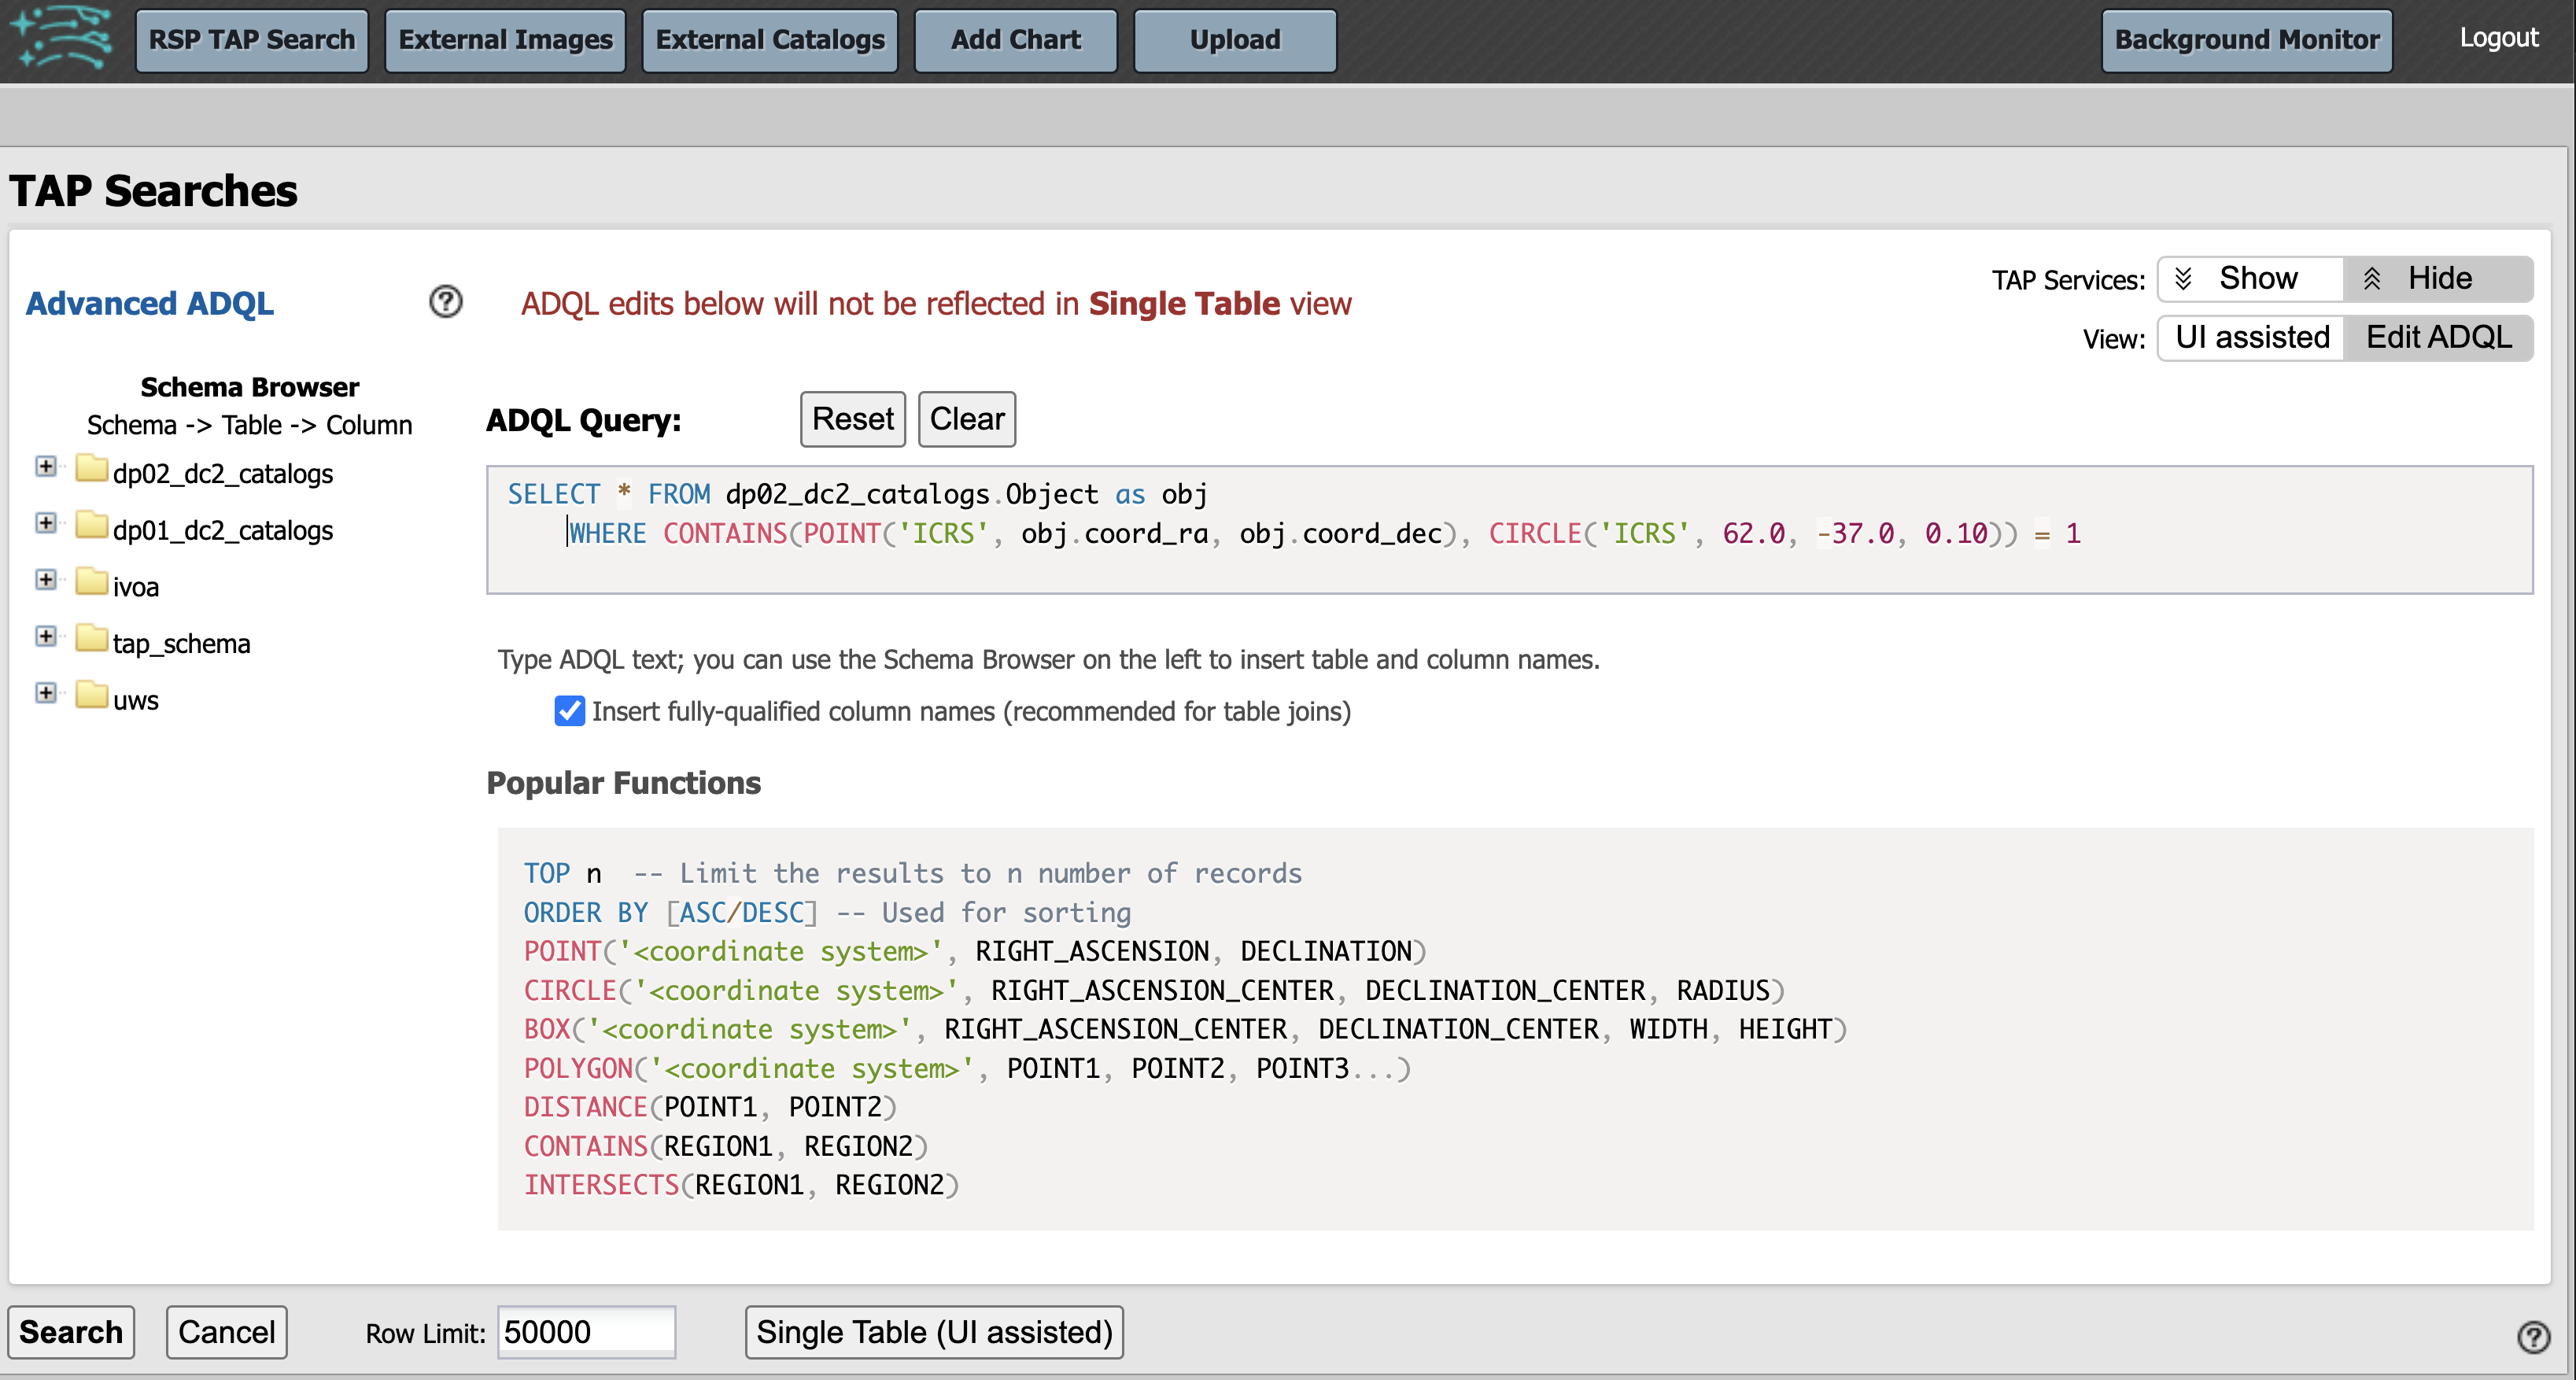
\includegraphics[width=5.16667in, ]{jira_imgs/4612.png}The
following screenshot shows the results, verifying that the query
returned 26,115 results, as expected.\\
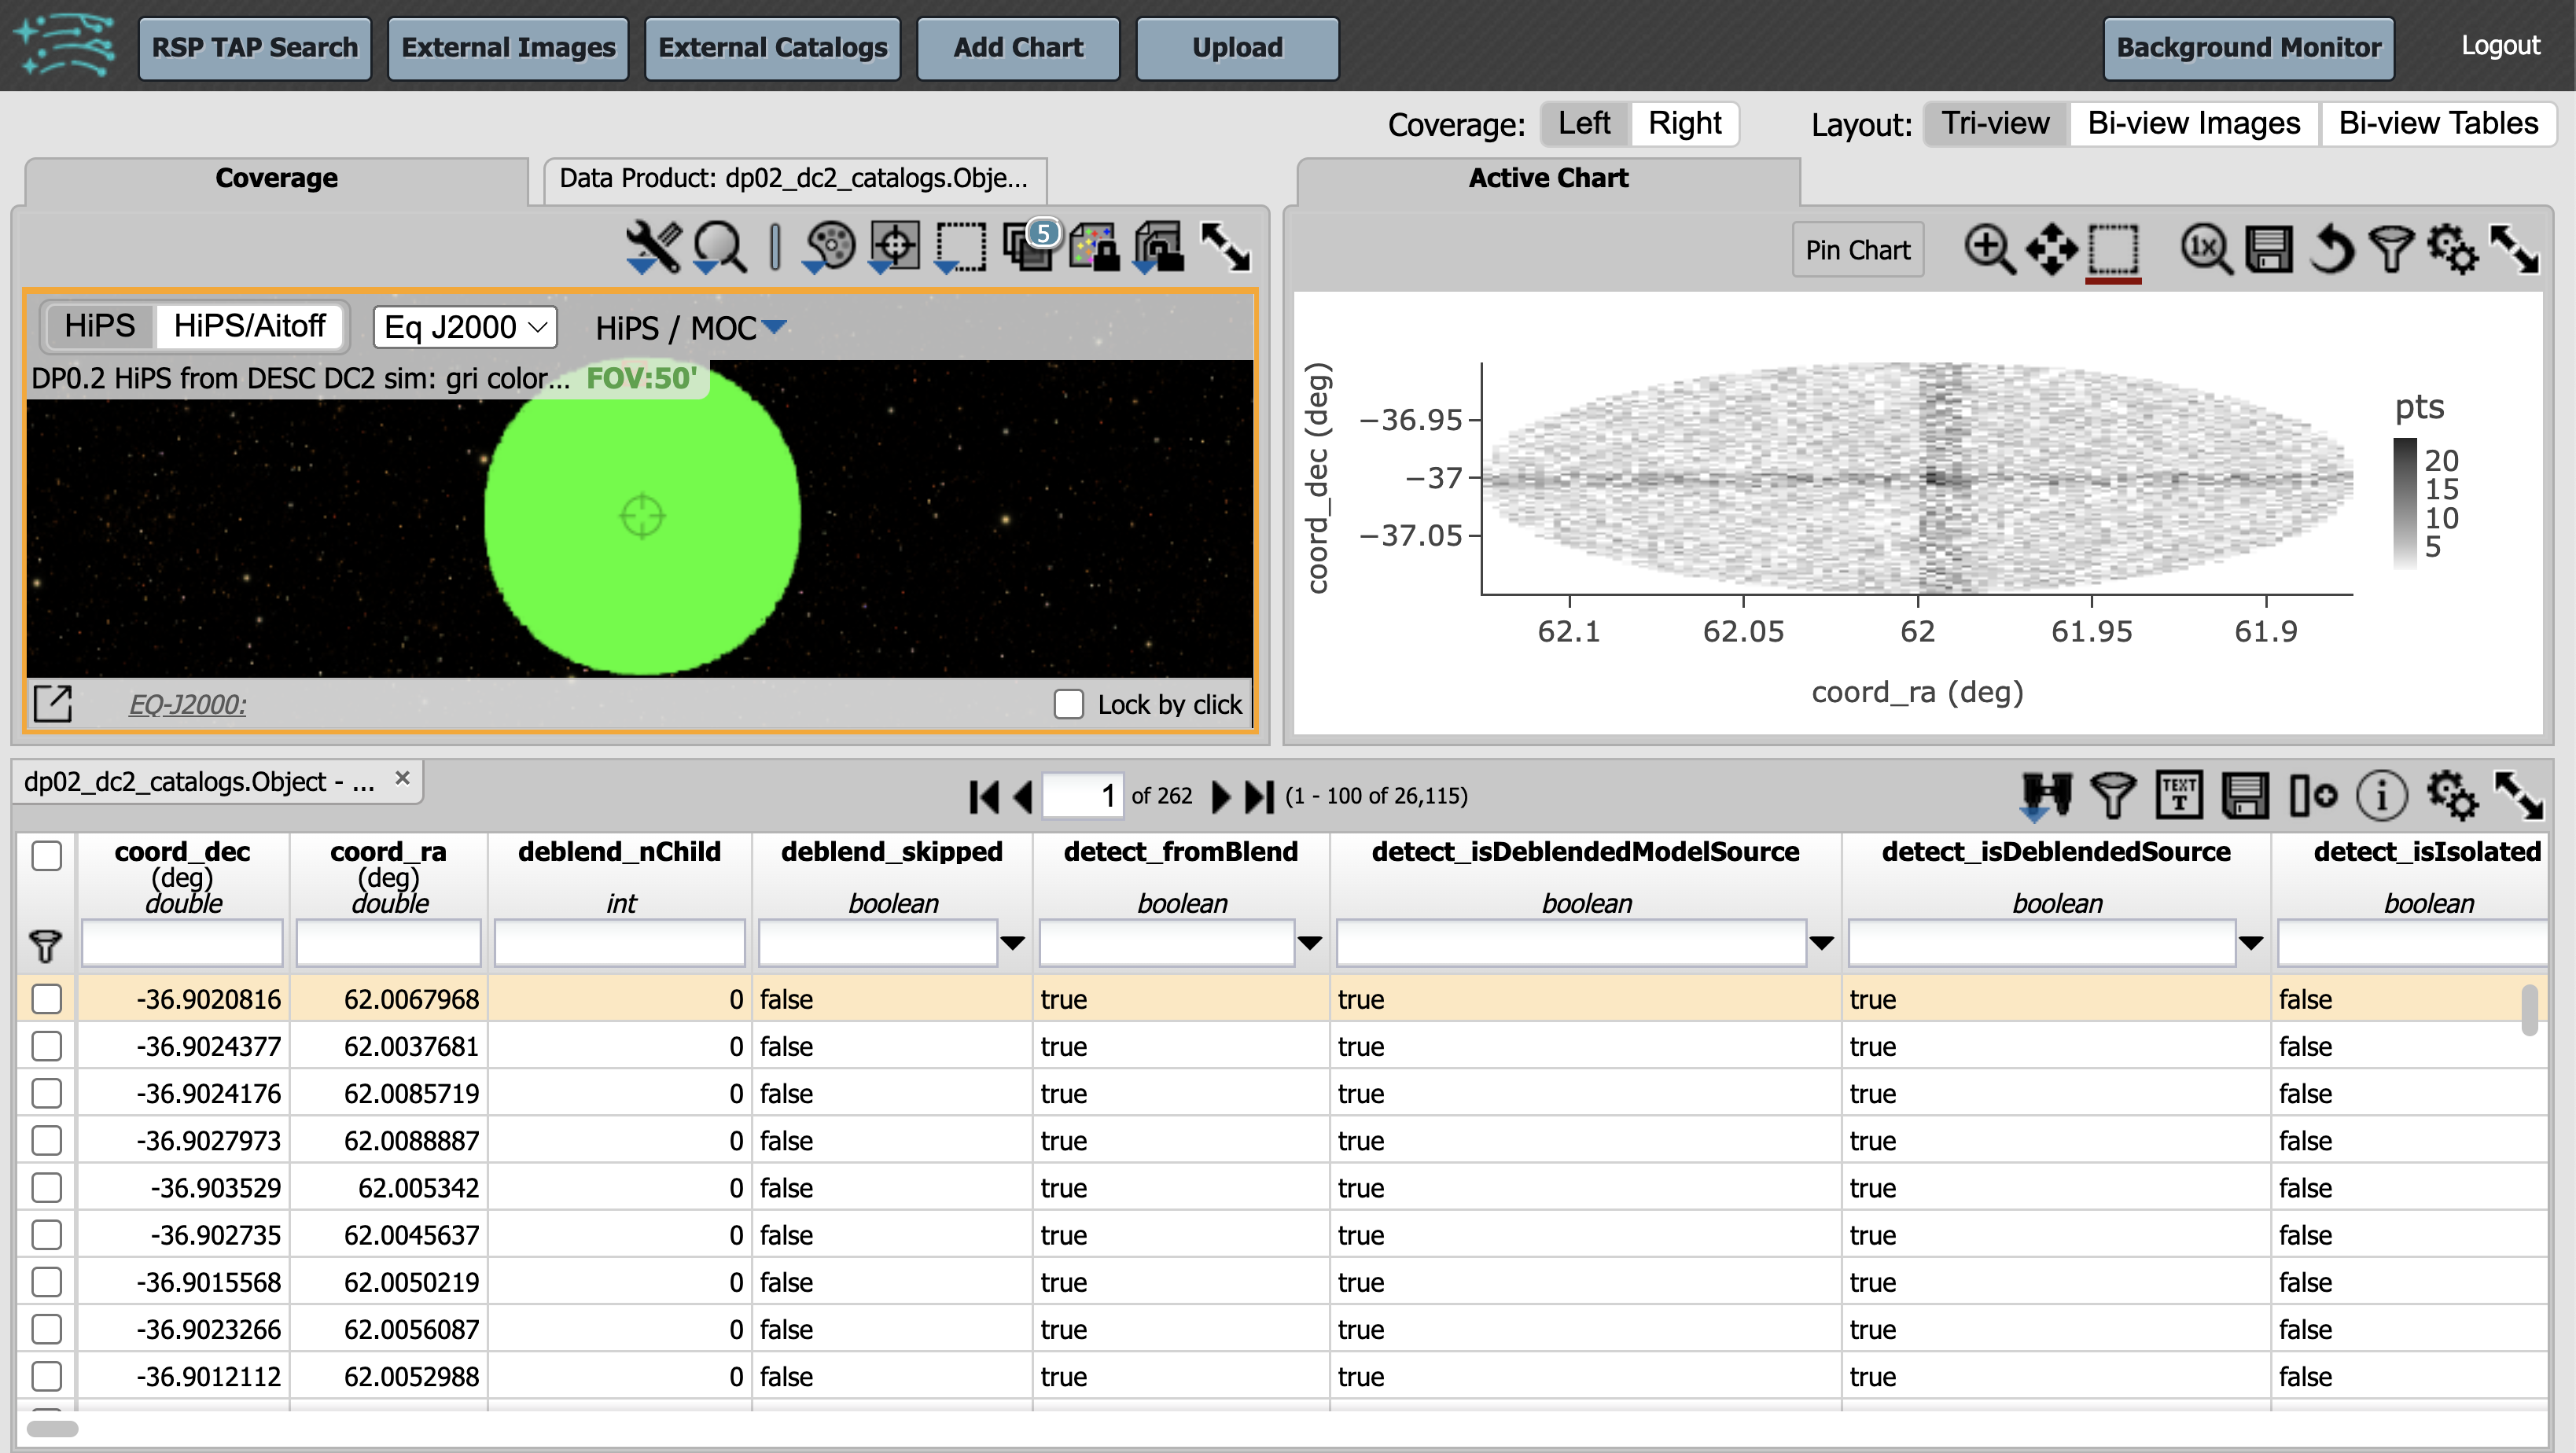
\includegraphics[width=5.20833in, ]{jira_imgs/4613.png}\\
We have thus demonstrated that catalogs can be queried via the Notebook,
Portal, and API aspects using ADQL queries.

}

\paragraph{ LVV-T40 - Verify implementation of Generate WCS for Visit Images }\mbox{}\\

Version \textbf{1}.
Status \textbf{Approved}.
Open  \href{https://jira.lsstcorp.org/secure/Tests.jspa#/testCase/LVV-T40}{\textit{ LVV-T40 } }
test case in Jira.

Verify that Processed Visit Images produced by the AP and DRP pipelines
include FITS WCS accurate to specified \textbf{astrometricAccuracy} over
the bounds of the image.

\textbf{ Preconditions}:\\


Execution status: {\bf  }

Final comment:\\



Detailed steps results LVV-C260-LVV-T40 LVV-E2962-3357:\\
{\bf Note:} Steps "Not Executed" and with No Result are not shown in this report.\\
\begin{tabular}{p{4cm}p{12cm}}
\toprule
Step LVV-E2962-1 & Step Execution Status: \textbf{ Pass } \\ \hline
\end{tabular}
 Description \\
{\footnotesize
Identify an appropriate repo containing processed HSC data for this
test.

}
\hdashrule[0.5ex]{\textwidth}{1pt}{3mm}
  Expected Result \\
{\footnotesize
A dataset with Processed Visit Images available.

}
\hdashrule[0.5ex]{\textwidth}{1pt}{3mm}
  Actual Result \\
{\footnotesize
For this test we use the most recent reprocessing of the Subaru+HSC RC2
dataset. The data were processed with the w\_2023\_32 pipelines.

}
\begin{tabular}{p{4cm}p{12cm}}
\toprule
Step LVV-E2962-2 & Step Execution Status: \textbf{ Pass } \\ \hline
\end{tabular}
 Description \\
{\footnotesize
Identify the path to the data repository, which we will refer to as
\textquotesingle DATA/path\textquotesingle, then execute the following:

}
\hdashrule[0.5ex]{\textwidth}{1pt}{3mm}
  Example Code \\
{\footnotesize
\begin{verbatim}
from lsst.daf.butler import Butler
repo = 'Data/path'
collection = 'collection'
butler = Butler(repo, collections=collection)
\end{verbatim}

}
\hdashrule[0.5ex]{\textwidth}{1pt}{3mm}
  Expected Result \\
{\footnotesize
Butler repo available for reading.

}
\hdashrule[0.5ex]{\textwidth}{1pt}{3mm}
  Actual Result \\
{\footnotesize
Butler access is as follows:\\
repo = \textquotesingle/repo/main\textquotesingle{}\\
rc2\_collection =
\textquotesingle HSC/runs/RC2/w\_2023\_32/DM-40356\textquotesingle{}\\
butler = Butler(repo, collections=rc2\_collection)

}
\begin{tabular}{p{4cm}p{12cm}}
\toprule
Step LVV-E2962-3 & Step Execution Status: \textbf{ Pass } \\ \hline
\end{tabular}
 Description \\
{\footnotesize
Select a single visit from the dataset, and extract its WCS object and
the source list.

}
\hdashrule[0.5ex]{\textwidth}{1pt}{3mm}
  Expected Result \\
{\footnotesize
A table containing detected sources, and a WCS object associated with
that catalog.

}
\hdashrule[0.5ex]{\textwidth}{1pt}{3mm}
  Actual Result \\
{\footnotesize
This was done 500 times, extracting the source list and WCS for 500
randomly-selected CCD/visit combinations from the repository.

}
\begin{tabular}{p{4cm}p{12cm}}
\toprule
Step LVV-E2962-4 & Step Execution Status: \textbf{ Pass } \\ \hline
\end{tabular}
 Description \\
{\footnotesize
Confirm that each CCD within the visit image contains at
least~\textbf{astrometricMinStandards~}astrometric standards that were
used in deriving the astrometric solution.

}
\hdashrule[0.5ex]{\textwidth}{1pt}{3mm}
  Expected Result \\
{\footnotesize
At least \textbf{astrometricMinStandards} from each CCD\textbf{~}were
used in determining the WCS solution.

}
\hdashrule[0.5ex]{\textwidth}{1pt}{3mm}
  Actual Result \\
{\footnotesize
It was confirmed that all CCDs selected had more than
astrometricMinStandards=5 standards used in their WCS solutions.\\
\strut \\
This was done using the following code to extract the number of
astrometric standards for each image:\\
\strut \\
astrom\_selection = np.where(src{[}'calib\_astrometry\_used'{]} ==
True)\\
num\_calib\_astrom.append(np.size(astrom\_selection))\\
\strut \\
In the end, we calculate the fraction of fields that met this
requirement, using:\\
wcsFlagsPercent = (np.size(np.where(num\_calib\_astrom \textgreater{}
5))/np.size(num\_calib\_astrom))*100.0*u.percent\\
\strut \\
The result (from the notebook) is:\\
Percentage of fields with \textgreater{} astrometricMinStandards=5:
100.0 \% -\/- True

}
\begin{tabular}{p{4cm}p{12cm}}
\toprule
Step LVV-E2962-5 & Step Execution Status: \textbf{ Pass } \\ \hline
\end{tabular}
 Description \\
{\footnotesize
Starting from the XY pixel coordinates of the sources, apply the WCS to
obtain RA, Dec coordinates.\\
\strut \\

}
\hdashrule[0.5ex]{\textwidth}{1pt}{3mm}
  Expected Result \\
{\footnotesize
A list of RA, Dec coordinates for all sources in the catalog.

}
\hdashrule[0.5ex]{\textwidth}{1pt}{3mm}
  Actual Result \\
{\footnotesize
Executed the following (for each CCD/visit) to create a list of RA, Dec
coords from XY:\\
\strut \\
xxx = src.getX()\\
yyy = src.getY()\\
radec = {[}wcs.pixelToSky(xxx{[}i{]}, yyy{[}i{]}) for i in
range(len(xxx)){]}\\
radec\_arr = np.array({[}(coo.getRa().asDegrees(),
coo.getDec().asDegrees()) for coo in radec{]})\\
\strut \\
This yields an array with RA, Dec coordinates.

}
\begin{tabular}{p{4cm}p{12cm}}
\toprule
Step LVV-E2962-6 & Step Execution Status: \textbf{ Pass } \\ \hline
\end{tabular}
 Description \\
{\footnotesize
We will assume that Gaia provides a source of "truth." Match the source
list to Gaia DR3, and calculate the positional offset between the test
data and the Gaia catalog.

}
\hdashrule[0.5ex]{\textwidth}{1pt}{3mm}
  Expected Result \\
{\footnotesize
A matched catalog of sources in common between the test source list and
Gaia DR3.

}
\hdashrule[0.5ex]{\textwidth}{1pt}{3mm}
  Actual Result \\
{\footnotesize
Used astroquery to extract Gaia sources, then Astropy utilities to match
the catalogs:\\
\strut \\
gaia\_mch = Gaia.query\_object\_async(coordinate=cen, width=width,
height=height)\\
sc\_src = SkyCoord(radec\_arr{[}:,0{]}*u.deg,
radec\_arr{[}:,1{]}*u.deg)\\
sc\_gaia = SkyCoord(gaia\_mch{[}'ra'{]}, gaia\_mch{[}'dec'{]})\\
src\_match = sc\_src.match\_to\_catalog\_sky(sc\_gaia)\\
sep\_match = src\_match{[}1{]}\\
\strut \\
Filtered the matched catalog to keep only matches with \textless0.5''
separation and with magnitude difference \textless{} 1.0 (relative to
the median magnitude difference of all sources, to account for different
filters):\\
\strut \\
okmch = (sep\_match.arcsec \textless{} 0.5)\\
matchsep = sep\_match{[}okmch{]}\\
\# Require the matches to have similar magnitudes:\\
gaia\_gmag = gaia\_mch{[}'phot\_g\_mean\_mag'{]}\\
magdiff =
src\_mag{[}okmch{]}{[}:,0{]}-gaia\_gmag{[}src\_match{[}0{]}{[}okmch{]}{]}\\
okmagdiff = (np.abs(magdiff - np.median(magdiff)) \textless{} 1.0)\\
okmatchsep = matchsep{[}okmagdiff{]}\\
\strut \\
This yields the final matched list.

}
\begin{tabular}{p{4cm}p{12cm}}
\toprule
Step LVV-E2962-7 & Step Execution Status: \textbf{ Pass } \\ \hline
\end{tabular}
 Description \\
{\footnotesize
Apply appropriate cuts to extract the optimal dataset for comparison,
then calculate statistics (median, 1-sigma range, etc.; also plot a
histogram) of the offsets in milliarcseconds. Confirm that the offset is
less than \textbf{astrometricAccuracy}.

}
\hdashrule[0.5ex]{\textwidth}{1pt}{3mm}
  Expected Result \\
{\footnotesize
Histogram and relevant statistics needed to confirm that the WCS
transformation is accurate.

}
\hdashrule[0.5ex]{\textwidth}{1pt}{3mm}
  Actual Result \\
{\footnotesize
Figures shown in the notebook. Rather than histograms, we used
comparisons of the various extracted parameters.\\
\strut \\
In addition to figures, we calculated the percentage of images that
satisfied the requirement on astrometricAccuracy. This was less than
100\% in all trials, likely due to some deep (or problematic) images
having few Gaia matches. The results printed in the notebook are as
follows:\\
\strut \\

\begin{verbatim}
Percentage of fields meeting the threshold:  95.99198396793587 %  --  False
\end{verbatim}

\hfill\break
Some brief exploration into reasons for a few images having large
astrometric residuals is included in the notebook
(`test\_LVV-T40\_T1240.ipynb`). These explorations suggest that the
small fraction of ``failing'' images are not meeting the requirement due
to inherent limitations in the data, and not a problem with the DM
algorithms. Thus, we grant this test a ``Pass.''

}
\begin{tabular}{p{4cm}p{12cm}}
\toprule
Step LVV-E2962-8 & Step Execution Status: \textbf{ Pass } \\ \hline
\end{tabular}
 Description \\
{\footnotesize
Repeat Step 5, but for subregions of the image, to confirm that the
accuracy criterion is met at all positions.

}
\hdashrule[0.5ex]{\textwidth}{1pt}{3mm}
  Expected Result \\
{\footnotesize
\textbf{astrometricAccuracy~}requirement is met over the entire image.

}
\hdashrule[0.5ex]{\textwidth}{1pt}{3mm}
  Actual Result \\
{\footnotesize
Upon examination, we find that many images have only \textless50 Gaia
matches over the entire frame. This is too few stars to get
statistically meaningful results from subregions, so we did not perform
this portion of the test.\\
\strut \\
We denote this test step as ``Pass,'' as it is likely the requirement
text will need to be removed or changed to account for the paucity of
Gaia sources in many fields, and it is thus likely that this step will
not be executed in the future. Nonetheless, this particular step does
not have any bearing on the overall requirement being tested.

}




% This appendix is put in as part of the template. You may edit and add to it.
% It is not overwritten by Docsteady.

\newpage
\appendix
\section{Documentation}
The verification process is defined in \citeds{LSE-160}.
The use of Docsteady to format Jira information in various test and planing documents is
described in \citeds{DMTN-140} and practical commands are given in \citeds{DMTN-178}.

\section{Acronyms used in this document}\label{sec:acronyms}
\input{acronyms.tex}

\newpage

% Uncomment this if Docsteady makes you additional appendix
%\input{DMTR-401.appendix.tex}

\end{document}
